%\pdfoutput=1
% Uncomment line above if submitting to arXiv and using pdflatex

% $Id: main.tex 33041 2013-03-25 16:12:53Z tgershon $
% ============================================================================
% Purpose: Template for LHCb documents
% Authors: Tomasz Skwarnicki, Roger Forty, Ulrik Egede
% Created on: 2010-09-24
% ============================================================================
\documentclass[12pt,a4paper]{article}
% For two column text, add "twocolumn" as an option to the document
% class. Also uncomment the two "onecolumn" and "twocolumn" lines
% around the title page below.

% Variables that controls behaviour
\usepackage{ifthen} % for conditional statements
\newboolean{pdflatex}
\setboolean{pdflatex}{true} % False for eps figures 
\usepackage{graphicx}
\usepackage{caption}
\usepackage{subcaption}
\newboolean{articletitles}
\setboolean{articletitles}{true} % False removes titles in references

\newboolean{uprightparticles}
\setboolean{uprightparticles}{false} %True for upright particle symbols

\newboolean{inbibliography}
\setboolean{inbibliography}{false} %True once you enter the bibliography

% THis file contains all the default packages and modifications for
% LHCb formatting

%% %%%%%%%%%%%%%%%%%%
%%  Page formatting
%% %%%%%%%%%%%%%%%%%%
\textheight=230mm
\textwidth=160mm
\oddsidemargin=7mm
\evensidemargin=-10mm
\topmargin=-10mm
\headsep=20mm
\columnsep=5mm
\addtolength{\belowcaptionskip}{0.5em}

\renewcommand{\textfraction}{0.01}
\renewcommand{\floatpagefraction}{0.99}
\renewcommand{\topfraction}{0.9}
\renewcommand{\bottomfraction}{0.9}


\setlength{\hoffset}{-2cm}
\setlength{\voffset}{-2cm}
% Page defaults ...
\topmargin=0.5cm
\oddsidemargin=2.5cm
\textwidth=16cm
\textheight=22cm
% Allow the page size to vary a bit ...
\raggedbottom
% To avoid Latex to be too fussy with line breaking ...
\sloppy

%% %%%%%%%%%%%%%%%%%%%%%%%
%% Packages to be used
%% %%%%%%%%%%%%%%%%%%%%%%% 
\usepackage{microtype}
\usepackage{lineno}  % for line numbering during review
\usepackage{xspace} % To avoid problems with missing or double spaces after
                    % predefined symbold


%% Graphics
\usepackage{graphicx}  % to include figures (can also use other packages)
\usepackage{color}
\usepackage{colortbl}
\graphicspath{{./figs/}} % Make Latex search fig subdir for figures

%% Math
\usepackage{amsmath} % Adds a large collection of math symbols
\usepackage{amssymb}
\usepackage{amsfonts}
\usepackage{upgreek} % Adds in support for greek letters in roman typeset

%% fix to allow peaceful coexistence of line numbering and
%% mathematical objects
%% http://www.latex-community.org/forum/viewtopic.php?f=5&t=163
%%
\newcommand*\patchAmsMathEnvironmentForLineno[1]{%
\expandafter\let\csname old#1\expandafter\endcsname\csname #1\endcsname
\expandafter\let\csname oldend#1\expandafter\endcsname\csname
end#1\endcsname
 \renewenvironment{#1}%
   {\linenomath\csname old#1\endcsname}%
   {\csname oldend#1\endcsname\endlinenomath}%
}
\newcommand*\patchBothAmsMathEnvironmentsForLineno[1]{%
  \patchAmsMathEnvironmentForLineno{#1}%
  \patchAmsMathEnvironmentForLineno{#1*}%
}
\AtBeginDocument{%
\patchBothAmsMathEnvironmentsForLineno{equation}%
\patchBothAmsMathEnvironmentsForLineno{align}%
\patchBothAmsMathEnvironmentsForLineno{flalign}%
\patchBothAmsMathEnvironmentsForLineno{alignat}%
\patchBothAmsMathEnvironmentsForLineno{gather}%
\patchBothAmsMathEnvironmentsForLineno{multline}%
}

% Get hyperlinks to captions and in references.
% These do not work with revtex. Use "hypertext" as class option instead.
\usepackage{hyperref}    % Hyperlinks in references
\usepackage[all]{hypcap} % Internal hyperlinks to floats.

%%% $Id: lhcb-symbols-def.tex 37587 2013-06-17 14:57:21Z roldeman $
%%% ======================================================================
%%% Purpose: Standard LHCb aliases
%%% Author: Originally Ulrik Egede, adapted by Tomasz Skwarnicki for templates,
%%% rewritten by Chris Parkes
%%% Maintainer : Ulrik Egede (2010 - 2012)
%%% =======================================================================

%%% To use this file outside the normal LHCb document environment, the
%%% following should be added in a preamble (before \begin{document}
%%%
%%%\usepackage{ifthen} 
%%%\newboolean{uprightparticles}
%%%\setboolean{uprightparticles}{false} %Set true for upright particle symbols
%%% \usepackage{xspace} 
%%% \usepackage{upgreek}

%%%%%%%%%%%%%%%%%%%%%%%%%%%%%%%%%%%%%%%%%%%%%%%%%%%%%%%%%%%%
%%%
%%% The following is to ensure that the template automatically can process
%%% this file.
%%%
%%% Add comments with at least three %%% preceding.
%%% Add new sections with one % preceding
%%% Add new subsections with two %% preceding
%%%%%%%%%%%%%%%%%%%%%%%%%%%%%%%%%%%%%%%%%%%%%%%%%%%%%%%%%%%%

%%%%%%%%%%%%%
% Experiments
%%%%%%%%%%%%%
\def\lhcb {\mbox{LHCb}\xspace}
\def\atlas  {\mbox{ATLAS}\xspace}
\def\cms    {\mbox{CMS}\xspace}
\def\alice  {\mbox{ALICE}\xspace}
\def\babar  {\mbox{BaBar}\xspace}
\def\belle  {\mbox{Belle}\xspace}
\def\cleo   {\mbox{CLEO}\xspace}
\def\cdf    {\mbox{CDF}\xspace}
\def\dzero  {\mbox{D0}\xspace}
\def\aleph  {\mbox{ALEPH}\xspace}
\def\delphi {\mbox{DELPHI}\xspace}
\def\opal   {\mbox{OPAL}\xspace}
\def\lthree {\mbox{L3}\xspace}
\def\sld    {\mbox{SLD}\xspace}
%%%\def\argus  {\mbox{ARGUS}\xspace}
%%%\def\uaone  {\mbox{UA1}\xspace}
%%%\def\uatwo  {\mbox{UA2}\xspace}
%%%\def\ux85 {\mbox{UX85}\xspace}
\def\cern {\mbox{CERN}\xspace}
\def\lhc    {\mbox{LHC}\xspace}
\def\lep    {\mbox{LEP}\xspace}
\def\tevatron {Tevatron\xspace}

%% LHCb sub-detectors and sub-systems

%%%\def\pu     {PU\xspace}
\def\velo   {VELO\xspace}
\def\rich   {RICH\xspace}
\def\richone {RICH1\xspace}
\def\richtwo {RICH2\xspace}
\def\ttracker {TT\xspace}
\def\intr   {IT\xspace}
\def\st     {ST\xspace}
\def\ot     {OT\xspace}
%%%\def\Tone   {T1\xspace}
%%%\def\Ttwo   {T2\xspace}
%%%\def\Tthree {T3\xspace}
%%%\def\Mone   {M1\xspace}
%%%\def\Mtwo   {M2\xspace}
%%%\def\Mthree {M3\xspace}
%%%\def\Mfour  {M4\xspace}
%%%\def\Mfive  {M5\xspace}
\def\spd    {SPD\xspace}
\def\presh  {PS\xspace}
\def\ecal   {ECAL\xspace}
\def\hcal   {HCAL\xspace}
%%%\def\bcm    {BCM\xspace}

%%%\def\ode    {ODE\xspace}
%%%\def\daq    {DAQ\xspace}
%%%\def\tfc    {TFC\xspace}
%%%\def\ecs    {ECS\xspace}
%%%\def\lone   {L0\xspace}
%%%\def\hlt    {HLT\xspace}
%%%\def\hltone {HLT1\xspace}
%%%\def\hlttwo {HLT2\xspace}

%%% Upright (not slanted) Particles

\ifthenelse{\boolean{uprightparticles}}%
{\def\Palpha      {\ensuremath{\upalpha}\xspace}
 \def\Pbeta       {\ensuremath{\upbeta}\xspace}
 \def\Pgamma      {\ensuremath{\upgamma}\xspace}                 
 \def\Pdelta      {\ensuremath{\updelta}\xspace}                 
 \def\Pepsilon    {\ensuremath{\upepsilon}\xspace}                 
 \def\Pvarepsilon {\ensuremath{\upvarepsilon}\xspace}                 
 \def\Pzeta       {\ensuremath{\upzeta}\xspace}                 
 \def\Peta        {\ensuremath{\upeta}\xspace}                 
 \def\Ptheta      {\ensuremath{\uptheta}\xspace}                 
 \def\Pvartheta   {\ensuremath{\upvartheta}\xspace}                 
 \def\Piota       {\ensuremath{\upiota}\xspace}                 
 \def\Pkappa      {\ensuremath{\upkappa}\xspace}                 
 \def\Plambda     {\ensuremath{\uplambda}\xspace}                 
 \def\Pmu         {\ensuremath{\upmu}\xspace}                 
 \def\Pnu         {\ensuremath{\upnu}\xspace}                 
 \def\Pxi         {\ensuremath{\upxi}\xspace}                 
 \def\Ppi         {\ensuremath{\uppi}\xspace}                 
 \def\Pvarpi      {\ensuremath{\upvarpi}\xspace}                 
 \def\Prho        {\ensuremath{\uprho}\xspace}                 
 \def\Pvarrho     {\ensuremath{\upvarrho}\xspace}                 
 \def\Ptau        {\ensuremath{\uptau}\xspace}                 
 \def\Pupsilon    {\ensuremath{\upupsilon}\xspace}                 
 \def\Pphi        {\ensuremath{\upphi}\xspace}                 
 \def\Pvarphi     {\ensuremath{\upvarphi}\xspace}                 
 \def\Pchi        {\ensuremath{\upchi}\xspace}                 
 \def\Ppsi        {\ensuremath{\uppsi}\xspace}                 
 \def\Pomega      {\ensuremath{\upomega}\xspace}                 

 \def\PDelta      {\ensuremath{\Delta}\xspace}                 
 \def\PXi      {\ensuremath{\Xi}\xspace}                 
 \def\PLambda      {\ensuremath{\Lambda}\xspace}                 
 \def\PSigma      {\ensuremath{\Sigma}\xspace}                 
 \def\POmega      {\ensuremath{\Omega}\xspace}                 
 \def\PUpsilon      {\ensuremath{\Upsilon}\xspace}                 
 
 %\mathchardef\Deltares="7101
 %\mathchardef\Xi="7104
 %\mathchardef\Lambda="7103
 %\mathchardef\Sigma="7106
 %\mathchardef\Omega="710A


 \def\PA      {\ensuremath{\mathrm{A}}\xspace}                 
 \def\PB      {\ensuremath{\mathrm{B}}\xspace}                 
 \def\PC      {\ensuremath{\mathrm{C}}\xspace}                 
 \def\PD      {\ensuremath{\mathrm{D}}\xspace}                 
 \def\PE      {\ensuremath{\mathrm{E}}\xspace}                 
 \def\PF      {\ensuremath{\mathrm{F}}\xspace}                 
 \def\PG      {\ensuremath{\mathrm{G}}\xspace}                 
 \def\PH      {\ensuremath{\mathrm{H}}\xspace}                 
 \def\PI      {\ensuremath{\mathrm{I}}\xspace}                 
 \def\PJ      {\ensuremath{\mathrm{J}}\xspace}                 
 \def\PK      {\ensuremath{\mathrm{K}}\xspace}                 
 \def\PL      {\ensuremath{\mathrm{L}}\xspace}                 
 \def\PM      {\ensuremath{\mathrm{M}}\xspace}                 
 \def\PN      {\ensuremath{\mathrm{N}}\xspace}                 
 \def\PO      {\ensuremath{\mathrm{O}}\xspace}                 
 \def\PP      {\ensuremath{\mathrm{P}}\xspace}                 
 \def\PQ      {\ensuremath{\mathrm{Q}}\xspace}                 
 \def\PR      {\ensuremath{\mathrm{R}}\xspace}                 
 \def\PS      {\ensuremath{\mathrm{S}}\xspace}                 
 \def\PT      {\ensuremath{\mathrm{T}}\xspace}                 
 \def\PU      {\ensuremath{\mathrm{U}}\xspace}                 
 \def\PV      {\ensuremath{\mathrm{V}}\xspace}                 
 \def\PW      {\ensuremath{\mathrm{W}}\xspace}                 
 \def\PX      {\ensuremath{\mathrm{X}}\xspace}                 
 \def\PY      {\ensuremath{\mathrm{Y}}\xspace}                 
 \def\PZ      {\ensuremath{\mathrm{Z}}\xspace}                 
 \def\Pa      {\ensuremath{\mathrm{a}}\xspace}                 
 \def\Pb      {\ensuremath{\mathrm{b}}\xspace}                 
 \def\Pc      {\ensuremath{\mathrm{c}}\xspace}                 
 \def\Pd      {\ensuremath{\mathrm{d}}\xspace}                 
 \def\Pe      {\ensuremath{\mathrm{e}}\xspace}                 
 \def\Pf      {\ensuremath{\mathrm{f}}\xspace}                 
 \def\Pg      {\ensuremath{\mathrm{g}}\xspace}                 
 \def\Ph      {\ensuremath{\mathrm{h}}\xspace}                 
 \def\Pi      {\ensuremath{\mathrm{i}}\xspace}                 
 \def\Pj      {\ensuremath{\mathrm{j}}\xspace}                 
 \def\Pk      {\ensuremath{\mathrm{k}}\xspace}                 
 \def\Pl      {\ensuremath{\mathrm{l}}\xspace}                 
 \def\Pm      {\ensuremath{\mathrm{m}}\xspace}                 
 \def\Pn      {\ensuremath{\mathrm{n}}\xspace}                 
 \def\Po      {\ensuremath{\mathrm{o}}\xspace}                 
 \def\Pp      {\ensuremath{\mathrm{p}}\xspace}                 
 \def\Pq      {\ensuremath{\mathrm{q}}\xspace}                 
 \def\Pr      {\ensuremath{\mathrm{r}}\xspace}                 
 \def\Ps      {\ensuremath{\mathrm{s}}\xspace}                 
 \def\Pt      {\ensuremath{\mathrm{t}}\xspace}                 
 \def\Pu      {\ensuremath{\mathrm{u}}\xspace}                 
 \def\Pv      {\ensuremath{\mathrm{v}}\xspace}                 
 \def\Pw      {\ensuremath{\mathrm{w}}\xspace}                 
 \def\Px      {\ensuremath{\mathrm{x}}\xspace}                 
 \def\Py      {\ensuremath{\mathrm{y}}\xspace}                 
 \def\Pz      {\ensuremath{\mathrm{z}}\xspace}                 
}
{\def\Palpha      {\ensuremath{\alpha}\xspace}
 \def\Pbeta       {\ensuremath{\beta}\xspace}
 \def\Pgamma      {\ensuremath{\gamma}\xspace}                 
 \def\Pdelta      {\ensuremath{\delta}\xspace}                 
 \def\Pepsilon    {\ensuremath{\epsilon}\xspace}                 
 \def\Pvarepsilon {\ensuremath{\varepsilon}\xspace}                 
 \def\Pzeta       {\ensuremath{\zeta}\xspace}                 
 \def\Peta        {\ensuremath{\eta}\xspace}                 
 \def\Ptheta      {\ensuremath{\theta}\xspace}                 
 \def\Pvartheta   {\ensuremath{\vartheta}\xspace}                 
 \def\Piota       {\ensuremath{\iota}\xspace}                 
 \def\Pkappa      {\ensuremath{\kappa}\xspace}                 
 \def\Plambda     {\ensuremath{\lambda}\xspace}                 
 \def\Pmu         {\ensuremath{\mu}\xspace}                 
 \def\Pnu         {\ensuremath{\nu}\xspace}                 
 \def\Pxi         {\ensuremath{\xi}\xspace}                 
 \def\Ppi         {\ensuremath{\pi}\xspace}                 
 \def\Pvarpi      {\ensuremath{\varpi}\xspace}                 
 \def\Prho        {\ensuremath{\rho}\xspace}                 
 \def\Pvarrho     {\ensuremath{\varrho}\xspace}                 
 \def\Ptau        {\ensuremath{\tau}\xspace}                 
 \def\Pupsilon    {\ensuremath{\upsilon}\xspace}                 
 \def\Pphi        {\ensuremath{\phi}\xspace}                 
 \def\Pvarphi     {\ensuremath{\varphi}\xspace}                 
 \def\Pchi        {\ensuremath{\chi}\xspace}                 
 \def\Ppsi        {\ensuremath{\psi}\xspace}                 
 \def\Pomega      {\ensuremath{\omega}\xspace}                 
 \mathchardef\PDelta="7101
 \mathchardef\PXi="7104
 \mathchardef\PLambda="7103
 \mathchardef\PSigma="7106
 \mathchardef\POmega="710A
 \mathchardef\PUpsilon="7107
 \def\PA      {\ensuremath{A}\xspace}                 
 \def\PB      {\ensuremath{B}\xspace}                 
 \def\PC      {\ensuremath{C}\xspace}                 
 \def\PD      {\ensuremath{D}\xspace}                 
 \def\PE      {\ensuremath{E}\xspace}                 
 \def\PF      {\ensuremath{F}\xspace}                 
 \def\PG      {\ensuremath{G}\xspace}                 
 \def\PH      {\ensuremath{H}\xspace}                 
 \def\PI      {\ensuremath{I}\xspace}                 
 \def\PJ      {\ensuremath{J}\xspace}                 
 \def\PK      {\ensuremath{K}\xspace}                 
 \def\PL      {\ensuremath{L}\xspace}                 
 \def\PM      {\ensuremath{M}\xspace}                 
 \def\PN      {\ensuremath{N}\xspace}                 
 \def\PO      {\ensuremath{O}\xspace}                 
 \def\PP      {\ensuremath{P}\xspace}                 
 \def\PQ      {\ensuremath{Q}\xspace}                 
 \def\PR      {\ensuremath{R}\xspace}                 
 \def\PS      {\ensuremath{S}\xspace}                 
 \def\PT      {\ensuremath{T}\xspace}                 
 \def\PU      {\ensuremath{U}\xspace}                 
 \def\PV      {\ensuremath{V}\xspace}                 
 \def\PW      {\ensuremath{W}\xspace}                 
 \def\PX      {\ensuremath{X}\xspace}                 
 \def\PY      {\ensuremath{Y}\xspace}                 
 \def\PZ      {\ensuremath{Z}\xspace}                 
 \def\Pa      {\ensuremath{a}\xspace}                 
 \def\Pb      {\ensuremath{b}\xspace}                 
 \def\Pc      {\ensuremath{c}\xspace}                 
 \def\Pd      {\ensuremath{d}\xspace}                 
 \def\Pe      {\ensuremath{e}\xspace}                 
 \def\Pf      {\ensuremath{f}\xspace}                 
 \def\Pg      {\ensuremath{g}\xspace}                 
 \def\Ph      {\ensuremath{h}\xspace}                 
 \def\Pi      {\ensuremath{i}\xspace}                 
 \def\Pj      {\ensuremath{j}\xspace}                 
 \def\Pk      {\ensuremath{k}\xspace}                 
 \def\Pl      {\ensuremath{l}\xspace}                 
 \def\Pm      {\ensuremath{m}\xspace}                 
 \def\Pn      {\ensuremath{n}\xspace}                 
 \def\Po      {\ensuremath{o}\xspace}                 
 \def\Pp      {\ensuremath{p}\xspace}                 
 \def\Pq      {\ensuremath{q}\xspace}                 
 \def\Pr      {\ensuremath{r}\xspace}                 
 \def\Ps      {\ensuremath{s}\xspace}                 
 \def\Pt      {\ensuremath{t}\xspace}                 
 \def\Pu      {\ensuremath{u}\xspace}                 
 \def\Pv      {\ensuremath{v}\xspace}                 
 \def\Pw      {\ensuremath{w}\xspace}                 
 \def\Px      {\ensuremath{x}\xspace}                 
 \def\Py      {\ensuremath{y}\xspace}                 
 \def\Pz      {\ensuremath{z}\xspace}                 
}

%%%%%%%%%%%%%%%%%%%%%%%%%%%%%%%%%%%%%%%%%%%%%%%
% Particles

%% Leptons

\let\emi\en
\def\electron   {\ensuremath{\Pe}\xspace}
\def\en         {\ensuremath{\Pe^-}\xspace}   % electron negative (\em is taken)
\def\ep         {\ensuremath{\Pe^+}\xspace}
\def\epm        {\ensuremath{\Pe^\pm}\xspace} 
\def\epem       {\ensuremath{\Pe^+\Pe^-}\xspace}
%%%\def\ee         {\ensuremath{\Pe^-\Pe^-}\xspace}

\def\mmu        {\ensuremath{\Pmu}\xspace}
\def\mup        {\ensuremath{\Pmu^+}\xspace}
\def\mun        {\ensuremath{\Pmu^-}\xspace} % muon negative (\mum is taken)
\def\mumu       {\ensuremath{\Pmu^+\Pmu^-}\xspace}
\def\mtau       {\ensuremath{\Ptau}\xspace}

\def\taup       {\ensuremath{\Ptau^+}\xspace}
\def\taum       {\ensuremath{\Ptau^-}\xspace}
\def\tautau     {\ensuremath{\Ptau^+\Ptau^-}\xspace}

\def\ellm       {\ensuremath{\ell^-}\xspace}
\def\ellp       {\ensuremath{\ell^+}\xspace}
%%%\def\ellell     {\ensuremath{\ell^+ \ell^-}\xspace}

\def\neu        {\ensuremath{\Pnu}\xspace}
\def\neub       {\ensuremath{\overline{\Pnu}}\xspace}
%%%\def\nuenueb    {\ensuremath{\neu\neub}\xspace}
\def\neue       {\ensuremath{\neu_e}\xspace}
\def\neueb      {\ensuremath{\neub_e}\xspace}
%%%\def\neueneueb  {\ensuremath{\neue\neueb}\xspace}
\def\neum       {\ensuremath{\neu_\mu}\xspace}
\def\neumb      {\ensuremath{\neub_\mu}\xspace}
%%%\def\neumneumb  {\ensuremath{\neum\neumb}\xspace}
\def\neut       {\ensuremath{\neu_\tau}\xspace}
\def\neutb      {\ensuremath{\neub_\tau}\xspace}
%%%\def\neutneutb  {\ensuremath{\neut\neutb}\xspace}
\def\neul       {\ensuremath{\neu_\ell}\xspace}
\def\neulb      {\ensuremath{\neub_\ell}\xspace}
%%%\def\neulneulb  {\ensuremath{\neul\neulb}\xspace}

%% Gauge bosons and scalars

\def\g      {\ensuremath{\Pgamma}\xspace}
\def\H      {\ensuremath{\PH^0}\xspace}
\def\Hp     {\ensuremath{\PH^+}\xspace}
\def\Hm     {\ensuremath{\PH^-}\xspace}
\def\Hpm    {\ensuremath{\PH^\pm}\xspace}
\def\W      {\ensuremath{\PW}\xspace}
\def\Wp     {\ensuremath{\PW^+}\xspace}
\def\Wm     {\ensuremath{\PW^-}\xspace}
\def\Wpm    {\ensuremath{\PW^\pm}\xspace}
\def\Z      {\ensuremath{\PZ}\xspace}

%% Quarks

\def\quark     {\ensuremath{\Pq}\xspace}
\def\quarkbar  {\ensuremath{\overline \quark}\xspace}
\def\qqbar     {\ensuremath{\quark\quarkbar}\xspace}
\def\uquark    {\ensuremath{\Pu}\xspace}
\def\uquarkbar {\ensuremath{\overline \uquark}\xspace}
\def\uubar     {\ensuremath{\uquark\uquarkbar}\xspace}
\def\dquark    {\ensuremath{\Pd}\xspace}
\def\dquarkbar {\ensuremath{\overline \dquark}\xspace}
\def\ddbar     {\ensuremath{\dquark\dquarkbar}\xspace}
\def\squark    {\ensuremath{\Ps}\xspace}
\def\squarkbar {\ensuremath{\overline \squark}\xspace}
\def\ssbar     {\ensuremath{\squark\squarkbar}\xspace}
\def\cquark    {\ensuremath{\Pc}\xspace}
\def\cquarkbar {\ensuremath{\overline \cquark}\xspace}
\def\ccbar     {\ensuremath{\cquark\cquarkbar}\xspace}
\def\bquark    {\ensuremath{\Pb}\xspace}
\def\bquarkbar {\ensuremath{\overline \bquark}\xspace}
\def\bbbar     {\ensuremath{\bquark\bquarkbar}\xspace}
\def\tquark    {\ensuremath{\Pt}\xspace}
\def\tquarkbar {\ensuremath{\overline \tquark}\xspace}
\def\ttbar     {\ensuremath{\tquark\tquarkbar}\xspace}

%% Light mesons

\def\pion  {\ensuremath{\Ppi}\xspace}
\def\piz   {\ensuremath{\pion^0}\xspace}
\def\pizs  {\ensuremath{\pion^0\mbox\,\rm{s}}\xspace}
%%%\def\ppz   {\ensuremath{\pion^0\pion^0}\xspace}
\def\pip   {\ensuremath{\pion^+}\xspace}
\def\pim   {\ensuremath{\pion^-}\xspace}
%%%\def\pipi  {\ensuremath{\pion^+\pion^-}\xspace}
\def\pipm  {\ensuremath{\pion^\pm}\xspace}
\def\pimp  {\ensuremath{\pion^\mp}\xspace}

\def\kaon  {\ensuremath{\PK}\xspace}
%%% do NOT use ensuremath here
  \def\Kbar  {\kern 0.2em\overline{\kern -0.2em \PK}{}\xspace}
\def\Kb    {\ensuremath{\Kbar}\xspace}
\def\Kz    {\ensuremath{\kaon^0}\xspace}
\def\Kzb   {\ensuremath{\Kbar^0}\xspace}
%%%\def\KzKzb {\ensuremath{\Kz \kern -0.16em \Kzb}\xspace}
\def\Kp    {\ensuremath{\kaon^+}\xspace}
\def\Km    {\ensuremath{\kaon^-}\xspace}
\def\Kpm   {\ensuremath{\kaon^\pm}\xspace}
\def\Kmp   {\ensuremath{\kaon^\mp}\xspace}
%%%\def\KpKm  {\ensuremath{\Kp \kern -0.16em \Km}\xspace}
\def\KS    {\ensuremath{\kaon^0_{\rm\scriptscriptstyle S}}\xspace} 
\def\KL    {\ensuremath{\kaon^0_{\rm\scriptscriptstyle L}}\xspace} 
\def\Kstarz  {\ensuremath{\kaon^{*0}}\xspace}
\def\Kstarzb {\ensuremath{\Kbar^{*0}}\xspace}
\def\Kstar   {\ensuremath{\kaon^*}\xspace}
\def\Kstarb  {\ensuremath{\Kbar^*}\xspace}
\def\Kstarp  {\ensuremath{\kaon^{*+}}\xspace}
\def\Kstarm  {\ensuremath{\kaon^{*-}}\xspace}
\def\Kstarpm {\ensuremath{\kaon^{*\pm}}\xspace}
\def\Kstarmp {\ensuremath{\kaon^{*\mp}}\xspace}

\newcommand{\etapr}{\ensuremath{\Peta^{\prime}}\xspace}

%% Heavy mesons

%%% do NOT use ensuremath here
  \def\Dbar    {\kern 0.2em\overline{\kern -0.2em \PD}{}\xspace}
\def\D       {\ensuremath{\PD}\xspace}
\def\Db      {\ensuremath{\Dbar}\xspace}
\def\Dz      {\ensuremath{\D^0}\xspace}
\def\Dzb     {\ensuremath{\Dbar^0}\xspace}
%%%\def\DzDzb   {\ensuremath{\Dz {\kern -0.16em \Dzb}}\xspace}
\def\Dp      {\ensuremath{\D^+}\xspace}
\def\Dm      {\ensuremath{\D^-}\xspace}
\def\Dpm     {\ensuremath{\D^\pm}\xspace}
\def\Dmp     {\ensuremath{\D^\mp}\xspace}
%%%\def\DpDm    {\ensuremath{\Dp {\kern -0.16em \Dm}}\xspace}
\def\Dstar   {\ensuremath{\D^*}\xspace}
\def\Dstarb  {\ensuremath{\Dbar^*}\xspace}
\def\Dstarz  {\ensuremath{\D^{*0}}\xspace}
\def\Dstarzb {\ensuremath{\Dbar^{*0}}\xspace}
\def\Dstarp  {\ensuremath{\D^{*+}}\xspace}
\def\Dstarm  {\ensuremath{\D^{*-}}\xspace}
\def\Dstarpm {\ensuremath{\D^{*\pm}}\xspace}
\def\Dstarmp {\ensuremath{\D^{*\mp}}\xspace}
\def\Ds      {\ensuremath{\D^+_\squark}\xspace}
\def\Dsp     {\ensuremath{\D^+_\squark}\xspace}
\def\Dsm     {\ensuremath{\D^-_\squark}\xspace}
\def\Dspm    {\ensuremath{\D^{\pm}_\squark}\xspace}
\def\Dsmp    {\ensuremath{\D^{\mp}_\squark}\xspace}
\def\Dss     {\ensuremath{\D^{*+}_\squark}\xspace}
\def\Dssp    {\ensuremath{\D^{*+}_\squark}\xspace}
\def\Dssm    {\ensuremath{\D^{*-}_\squark}\xspace}
\def\Dsspm   {\ensuremath{\D^{*\pm}_\squark}\xspace}
\def\Dssmp   {\ensuremath{\D^{*\mp}_\squark}\xspace}

\def\B       {\ensuremath{\PB}\xspace}
%%% do NOT use ensuremath here
\def\Bbar    {\ensuremath{\kern 0.18em\overline{\kern -0.18em \PB}{}}\xspace}
\def\Bb      {\ensuremath{\Bbar}\xspace}
%%%\def\BBbar   {\ensuremath{\B\Bbar}\xspace} 
\def\Bz      {\ensuremath{\B^0}\xspace}
\def\Bzb     {\ensuremath{\Bbar^0}\xspace}
\def\Bu      {\ensuremath{\B^+}\xspace}
\def\Bub     {\ensuremath{\B^-}\xspace}
\def\Bp      {\ensuremath{\Bu}\xspace}
\def\Bm      {\ensuremath{\Bub}\xspace}
\def\Bpm     {\ensuremath{\B^\pm}\xspace}
\def\Bmp     {\ensuremath{\B^\mp}\xspace}
\def\Bd      {\ensuremath{\B^0}\xspace}
\def\Bs      {\ensuremath{\B^0_\squark}\xspace}
\def\Bsb     {\ensuremath{\Bbar^0_\squark}\xspace}
\def\Bdb     {\ensuremath{\Bbar^0}\xspace}
\def\Bc      {\ensuremath{\B_\cquark^+}\xspace}
\def\Bcp     {\ensuremath{\B_\cquark^+}\xspace}
\def\Bcm     {\ensuremath{\B_\cquark^-}\xspace}
\def\Bcpm    {\ensuremath{\B_\cquark^\pm}\xspace}

%% Onia

\def\jpsi     {\ensuremath{{\PJ\mskip -3mu/\mskip -2mu\Ppsi\mskip 2mu}}\xspace}
\def\psitwos  {\ensuremath{\Ppsi{(2S)}}\xspace}
\def\psiprpr  {\ensuremath{\Ppsi(3770)}\xspace}
\def\etac     {\ensuremath{\Peta_\cquark}\xspace}
\def\chiczero {\ensuremath{\Pchi_{\cquark 0}}\xspace}
\def\chicone  {\ensuremath{\Pchi_{\cquark 1}}\xspace}
\def\chictwo  {\ensuremath{\Pchi_{\cquark 2}}\xspace}
  %\mathchardef\Upsilon="7107
  \def\Y#1S{\ensuremath{\PUpsilon{(#1S)}}\xspace}% no space before {...}!
\def\OneS  {\Y1S}
\def\TwoS  {\Y2S}
\def\ThreeS{\Y3S}
\def\FourS {\Y4S}
\def\FiveS {\Y5S}

\def\chic  {\ensuremath{\Pchi_{c}}\xspace}

%% Baryons

\def\proton      {\ensuremath{\Pp}\xspace}
\def\antiproton  {\ensuremath{\overline \proton}\xspace}
\def\neutron     {\ensuremath{\Pn}\xspace}
\def\antineutron {\ensuremath{\overline \neutron}\xspace}

\def\Deltares {\ensuremath{\PDelta}\xspace}
\def\Deltaresbar{\ensuremath{\overline \Deltares}\xspace}
\def\Xires {\ensuremath{\PXi}\xspace}
\def\Xiresbar{\ensuremath{\overline \Xires}\xspace}
\def\Lz {\ensuremath{\PLambda}\xspace}
\def\Lbar {\ensuremath{\kern 0.1em\overline{\kern -0.1em\PLambda}}\xspace}
\def\Lambdares {\ensuremath{\PLambda}\xspace}
\def\Lambdaresbar{\ensuremath{\Lbar}\xspace}
\def\Sigmares {\ensuremath{\PSigma}\xspace}
\def\Sigmaresbar{\ensuremath{\overline \Sigmares}\xspace}
\def\Omegares {\ensuremath{\POmega^-}\xspace}
\def\Omegaresbar{\ensuremath{\overline{\POmega}^+}\xspace}

%%% do NOT use ensuremath here
 % \def\Deltabar{\kern 0.25em\overline{\kern -0.25em \Deltares}{}\xspace}
 % \def\Sigbar{\kern 0.2em\overline{\kern -0.2em \Sigma}{}\xspace}
 % \def\Xibar{\kern 0.2em\overline{\kern -0.2em \Xi}{}\xspace}
 % \def\Obar{\kern 0.2em\overline{\kern -0.2em \Omega}{}\xspace}
 % \def\Nbar{\kern 0.2em\overline{\kern -0.2em N}{}\xspace}
 % \def\Xb{\kern 0.2em\overline{\kern -0.2em X}{}\xspace}

\def\Lb      {\ensuremath{\Lz^0_\bquark}\xspace}
\def\Lbbar   {\ensuremath{\Lbar^0_\bquark}\xspace}
\def\Lc      {\ensuremath{\Lz^+_\cquark}\xspace}
\def\Lcbar   {\ensuremath{\Lbar^-_\cquark}\xspace}

%%%%%%%%%%%%%%%%%%
% Physics symbols
%%%%%%%%%%%%%%%%%

%% Decays
\def\BF         {{\ensuremath{\cal B}\xspace}}
\def\BRvis      {{\ensuremath{\BR_{\rm{vis}}}}}
\def\BR         {\BF}
\newcommand{\decay}[2]{\ensuremath{#1\!\to #2}\xspace}         % {\Pa}{\Pb \Pc}
\def\ra                 {\ensuremath{\rightarrow}\xspace}
\def\to                 {\ensuremath{\rightarrow}\xspace}

%% Lifetimes
\newcommand{\tauBs}{\ensuremath{\tau_{\Bs}}\xspace}
\newcommand{\tauBd}{\ensuremath{\tau_{\Bd}}\xspace}
\newcommand{\tauBz}{\ensuremath{\tau_{\Bz}}\xspace}
\newcommand{\tauBu}{\ensuremath{\tau_{\Bp}}\xspace}
\newcommand{\tauDp}{\ensuremath{\tau_{\Dp}}\xspace}
\newcommand{\tauDz}{\ensuremath{\tau_{\Dz}}\xspace}
\newcommand{\tauL}{\ensuremath{\tau_{\rm L}}\xspace}
\newcommand{\tauH}{\ensuremath{\tau_{\rm H}}\xspace}

%% Masses
\newcommand{\mBd}{\ensuremath{m_{\Bd}}\xspace}
\newcommand{\mBp}{\ensuremath{m_{\Bp}}\xspace}
\newcommand{\mBs}{\ensuremath{m_{\Bs}}\xspace}
\newcommand{\mBc}{\ensuremath{m_{\Bc}}\xspace}
\newcommand{\mLb}{\ensuremath{m_{\Lb}}\xspace}

%% EW theory, groups
\def\grpsuthree {\ensuremath{\mathrm{SU}(3)}\xspace}
\def\grpsutw    {\ensuremath{\mathrm{SU}(2)}\xspace}
\def\grpuone    {\ensuremath{\mathrm{U}(1)}\xspace}

\def\ssqtw {\ensuremath{\sin^{2}\!\theta_{\mathrm{W}}}\xspace}
\def\csqtw {\ensuremath{\cos^{2}\!\theta_{\mathrm{W}}}\xspace}
\def\stw   {\ensuremath{\sin\theta_{\mathrm{W}}}\xspace}
\def\ctw   {\ensuremath{\cos\theta_{\mathrm{W}}}\xspace}
\def\ssqtwef {\ensuremath{{\sin}^{2}\theta_{\mathrm{W}}^{\mathrm{eff}}}\xspace}
\def\csqtwef {\ensuremath{{\cos}^{2}\theta_{\mathrm{W}}^{\mathrm{eff}}}\xspace}
\def\stwef {\ensuremath{\sin\theta_{\mathrm{W}}^{\mathrm{eff}}}\xspace}
\def\ctwef {\ensuremath{\cos\theta_{\mathrm{W}}^{\mathrm{eff}}}\xspace}
\def\gv    {\ensuremath{g_{\mbox{\tiny V}}}\xspace}
\def\ga    {\ensuremath{g_{\mbox{\tiny A}}}\xspace}

\def\order   {\ensuremath{\mathcal{O}}\xspace}
\def\ordalph {\ensuremath{\mathcal{O}(\alpha)}\xspace}
\def\ordalsq {\ensuremath{\mathcal{O}(\alpha^{2})}\xspace}
\def\ordalcb {\ensuremath{\mathcal{O}(\alpha^{3})}\xspace}

%% QCD parameters
\newcommand{\as}{\ensuremath{\alpha_s}\xspace}
\newcommand{\MSb}{\ensuremath{\overline{\mathrm{MS}}}\xspace}
\newcommand{\lqcd}{\ensuremath{\Lambda_{\mathrm{QCD}}}\xspace}
\def\qsq       {\ensuremath{q^2}\xspace}

%% CKM, CP violation

\def\eps   {\ensuremath{\varepsilon}\xspace}
\def\epsK  {\ensuremath{\varepsilon_K}\xspace}
\def\epsB  {\ensuremath{\varepsilon_B}\xspace}
\def\epsp  {\ensuremath{\varepsilon^\prime_K}\xspace}

\def\CP                {\ensuremath{C\!P}\xspace}
\def\CPT               {\ensuremath{C\!PT}\xspace}

\def\rhobar {\ensuremath{\overline \rho}\xspace}
\def\etabar {\ensuremath{\overline \eta}\xspace}

\def\Vud  {\ensuremath{|V_{\uquark\dquark}|}\xspace}
\def\Vcd  {\ensuremath{|V_{\cquark\dquark}|}\xspace}
\def\Vtd  {\ensuremath{|V_{\tquark\dquark}|}\xspace}
\def\Vus  {\ensuremath{|V_{\uquark\squark}|}\xspace}
\def\Vcs  {\ensuremath{|V_{\cquark\squark}|}\xspace}
\def\Vts  {\ensuremath{|V_{\tquark\squark}|}\xspace}
\def\Vub  {\ensuremath{|V_{\uquark\bquark}|}\xspace}
\def\Vcb  {\ensuremath{|V_{\cquark\bquark}|}\xspace}
\def\Vtb  {\ensuremath{|V_{\tquark\bquark}|}\xspace}

%% Oscillations

\newcommand{\dm}{\ensuremath{\Delta m}\xspace}
\newcommand{\dms}{\ensuremath{\Delta m_{\squark}}\xspace}
\newcommand{\dmd}{\ensuremath{\Delta m_{\dquark}}\xspace}
\newcommand{\DG}{\ensuremath{\Delta\Gamma}\xspace}
\newcommand{\DGs}{\ensuremath{\Delta\Gamma_{\squark}}\xspace}
\newcommand{\DGd}{\ensuremath{\Delta\Gamma_{\dquark}}\xspace}
\newcommand{\Gs}{\ensuremath{\Gamma_{\squark}}\xspace}
\newcommand{\Gd}{\ensuremath{\Gamma_{\dquark}}\xspace}

\newcommand{\MBq}{\ensuremath{M_{\B_\quark}}\xspace}
\newcommand{\DGq}{\ensuremath{\Delta\Gamma_{\quark}}\xspace}
\newcommand{\Gq}{\ensuremath{\Gamma_{\quark}}\xspace}
\newcommand{\dmq}{\ensuremath{\Delta m_{\quark}}\xspace}
\newcommand{\GL}{\ensuremath{\Gamma_{\rm L}}\xspace}
\newcommand{\GH}{\ensuremath{\Gamma_{\rm H}}\xspace}

\newcommand{\DGsGs}{\ensuremath{\Delta\Gamma_{\squark}/\Gamma_{\squark}}\xspace}
\newcommand{\Delm}{\mbox{$\Delta m $}\xspace}
\newcommand{\ACP}{\ensuremath{{\cal A}^{\CP}}\xspace}
\newcommand{\Adir}{\ensuremath{{\cal A}^{\rm dir}}\xspace}
\newcommand{\Amix}{\ensuremath{{\cal A}^{\rm mix}}\xspace}
\newcommand{\ADelta}{\ensuremath{{\cal A}^\Delta}\xspace}
\newcommand{\phid}{\ensuremath{\phi_{\dquark}}\xspace}
\newcommand{\sinphid}{\ensuremath{\sin\!\phid}\xspace}
\newcommand{\phis}{\ensuremath{\phi_{\squark}}\xspace}
\newcommand{\betas}{\ensuremath{\beta_{\squark}}\xspace}
\newcommand{\sbetas}{\ensuremath{\sigma(\beta_{\squark})}\xspace}
\newcommand{\stbetas}{\ensuremath{\sigma(2\beta_{\squark})}\xspace}
\newcommand{\stphis}{\ensuremath{\sigma(\phi_{\squark})}\xspace}
\newcommand{\sinphis}{\ensuremath{\sin\!\phis}\xspace}

%% Tagging
\newcommand{\edet}{{\ensuremath{\varepsilon_{\rm det}}}\xspace}
\newcommand{\erec}{{\ensuremath{\varepsilon_{\rm rec/det}}}\xspace}
\newcommand{\esel}{{\ensuremath{\varepsilon_{\rm sel/rec}}}\xspace}
\newcommand{\etrg}{{\ensuremath{\varepsilon_{\rm trg/sel}}}\xspace}
\newcommand{\etot}{{\ensuremath{\varepsilon_{\rm tot}}}\xspace}

\newcommand{\mistag}{\ensuremath{\omega}\xspace}
\newcommand{\wcomb}{\ensuremath{\omega^{\rm comb}}\xspace}
\newcommand{\etag}{{\ensuremath{\varepsilon_{\rm tag}}}\xspace}
\newcommand{\etagcomb}{{\ensuremath{\varepsilon_{\rm tag}^{\rm comb}}}\xspace}
\newcommand{\effeff}{\ensuremath{\varepsilon_{\rm eff}}\xspace}
\newcommand{\effeffcomb}{\ensuremath{\varepsilon_{\rm eff}^{\rm comb}}\xspace}
\newcommand{\efftag}{{\ensuremath{\etag(1-2\omega)^2}}\xspace}
\newcommand{\effD}{{\ensuremath{\etag D^2}}\xspace}

\newcommand{\etagprompt}{{\ensuremath{\varepsilon_{\rm tag}^{\rm Pr}}}\xspace}
\newcommand{\etagLL}{{\ensuremath{\varepsilon_{\rm tag}^{\rm LL}}}\xspace}

%% Key decay channels

\def\BdToKstmm    {\decay{\Bd}{\Kstarz\mup\mun}}
\def\BdbToKstmm   {\decay{\Bdb}{\Kstarzb\mup\mun}}

\def\BsToJPsiPhi  {\decay{\Bs}{\jpsi\phi}}
\def\BdToJPsiKst  {\decay{\Bd}{\jpsi\Kstarz}}
\def\BdbToJPsiKst {\decay{\Bdb}{\jpsi\Kstarzb}}

\def\BsPhiGam     {\decay{\Bs}{\phi \g}}
\def\BdKstGam     {\decay{\Bd}{\Kstarz \g}}

\def\BTohh        {\decay{\B}{\Ph^+ \Ph'^-}}
\def\BdTopipi     {\decay{\Bd}{\pip\pim}}
\def\BdToKpi      {\decay{\Bd}{\Kp\pim}}
\def\BsToKK       {\decay{\Bs}{\Kp\Km}}
\def\BsTopiK      {\decay{\Bs}{\pip\Km}}

%% Rare decays
\def\BdKstee  {\decay{\Bd}{\Kstarz\epem}}
\def\BdbKstee {\decay{\Bdb}{\Kstarzb\epem}}
\def\bsll     {\decay{\bquark}{\squark \ell^+ \ell^-}}
\def\AFB      {\ensuremath{A_{\mathrm{FB}}}\xspace}
\def\FL       {\ensuremath{F_{\mathrm{L}}}\xspace}
\def\AT#1     {\ensuremath{A_{\mathrm{T}}^{#1}}\xspace}           % 2
\def\btosgam  {\decay{\bquark}{\squark \g}}
\def\btodgam  {\decay{\bquark}{\dquark \g}}
\def\Bsmm     {\decay{\Bs}{\mup\mun}}
\def\Bdmm     {\decay{\Bd}{\mup\mun}}
\def\ctl       {\ensuremath{\cos{\theta_\ell}}\xspace}
\def\ctk       {\ensuremath{\cos{\theta_K}}\xspace}

%% Wilson coefficients and operators
\def\C#1      {\ensuremath{\mathcal{C}_{#1}}\xspace}                       % 9
\def\Cp#1     {\ensuremath{\mathcal{C}_{#1}^{'}}\xspace}                    % 7
\def\Ceff#1   {\ensuremath{\mathcal{C}_{#1}^{\mathrm{(eff)}}}\xspace}        % 9  
\def\Cpeff#1  {\ensuremath{\mathcal{C}_{#1}^{'\mathrm{(eff)}}}\xspace}       % 7
\def\Ope#1    {\ensuremath{\mathcal{O}_{#1}}\xspace}                       % 2
\def\Opep#1   {\ensuremath{\mathcal{O}_{#1}^{'}}\xspace}                    % 7

%% Charm

\def\xprime     {\ensuremath{x^{\prime}}\xspace}
\def\yprime     {\ensuremath{y^{\prime}}\xspace}
\def\ycp        {\ensuremath{y_{\CP}}\xspace}
\def\agamma     {\ensuremath{A_{\Gamma}}\xspace}
%%%\def\kpi        {\ensuremath{\PK\Ppi}\xspace}
%%%\def\kk         {\ensuremath{\PK\PK}\xspace}
%%%\def\dkpi       {\decay{\PD}{\PK\Ppi}}
%%%\def\dkk        {\decay{\PD}{\PK\PK}}
\def\dkpicf     {\decay{\Dz}{\Km\pip}}

%% QM
\newcommand{\bra}[1]{\ensuremath{\langle #1|}}             % {a}
\newcommand{\ket}[1]{\ensuremath{|#1\rangle}}              % {b}
\newcommand{\braket}[2]{\ensuremath{\langle #1|#2\rangle}} % {a}{b}

%%%%%%%%%%%%%%%%%%%%%%%%%%%%%%%%%%%%%%%%%%%%%%%%%%
% Units
%%%%%%%%%%%%%%%%%%%%%%%%%%%%%%%%%%%%%%%%%%%%%%%%%%
\newcommand{\unit}[1]{\ensuremath{\rm\,#1}\xspace}          % {kg}

%% Energy and momentum
\newcommand{\tev}{\ifthenelse{\boolean{inbibliography}}{\ensuremath{~T\kern -0.05em eV}\xspace}{\ensuremath{\mathrm{\,Te\kern -0.1em V}}\xspace}}
\newcommand{\gev}{\ensuremath{\mathrm{\,Ge\kern -0.1em V}}\xspace}
\newcommand{\mev}{\ensuremath{\mathrm{\,Me\kern -0.1em V}}\xspace}
\newcommand{\kev}{\ensuremath{\mathrm{\,ke\kern -0.1em V}}\xspace}
\newcommand{\ev}{\ensuremath{\mathrm{\,e\kern -0.1em V}}\xspace}
\newcommand{\gevc}{\ensuremath{{\mathrm{\,Ge\kern -0.1em V\!/}c}}\xspace}
\newcommand{\mevc}{\ensuremath{{\mathrm{\,Me\kern -0.1em V\!/}c}}\xspace}
\newcommand{\gevcc}{\ensuremath{{\mathrm{\,Ge\kern -0.1em V\!/}c^2}}\xspace}
\newcommand{\gevgevcccc}{\ensuremath{{\mathrm{\,Ge\kern -0.1em V^2\!/}c^4}}\xspace}
\newcommand{\mevcc}{\ensuremath{{\mathrm{\,Me\kern -0.1em V\!/}c^2}}\xspace}

%% Distance and area
\def\km   {\ensuremath{\rm \,km}\xspace}
\def\m    {\ensuremath{\rm \,m}\xspace}
\def\cm   {\ensuremath{\rm \,cm}\xspace}
\def\cma  {\ensuremath{{\rm \,cm}^2}\xspace}
\def\mm   {\ensuremath{\rm \,mm}\xspace}
\def\mma  {\ensuremath{{\rm \,mm}^2}\xspace}
\def\mum  {\ensuremath{\,\upmu\rm m}\xspace}
\def\muma {\ensuremath{\,\upmu\rm m^2}\xspace}
\def\nm   {\ensuremath{\rm \,nm}\xspace}
\def\fm   {\ensuremath{\rm \,fm}\xspace}
\def\barn{\ensuremath{\rm \,b}\xspace}
%%%\def\barnhyph{\ensuremath{\rm -b}\xspace}
\def\mbarn{\ensuremath{\rm \,mb}\xspace}
\def\mub{\ensuremath{\rm \,\upmu b}\xspace}
%%%\def\mbarnhyph{\ensuremath{\rm -mb}\xspace}
\def\nb {\ensuremath{\rm \,nb}\xspace}
\def\invnb {\ensuremath{\mbox{\,nb}^{-1}}\xspace}
\def\pb {\ensuremath{\rm \,pb}\xspace}
\def\invpb {\ensuremath{\mbox{\,pb}^{-1}}\xspace}
\def\fb   {\ensuremath{\mbox{\,fb}}\xspace}
\def\invfb   {\ensuremath{\mbox{\,fb}^{-1}}\xspace}

%% Time 
\def\sec  {\ensuremath{\rm {\,s}}\xspace}
\def\ms   {\ensuremath{{\rm \,ms}}\xspace}
\def\mus  {\ensuremath{\,\upmu{\rm s}}\xspace}
\def\ns   {\ensuremath{{\rm \,ns}}\xspace}
\def\ps   {\ensuremath{{\rm \,ps}}\xspace}
\def\fs   {\ensuremath{\rm \,fs}\xspace}

\def\mhz  {\ensuremath{{\rm \,MHz}}\xspace}
\def\khz  {\ensuremath{{\rm \,kHz}}\xspace}
\def\hz   {\ensuremath{{\rm \,Hz}}\xspace}

\def\invps{\ensuremath{{\rm \,ps^{-1}}}\xspace}

\def\yr   {\ensuremath{\rm \,yr}\xspace}
\def\hr   {\ensuremath{\rm \,hr}\xspace}

%% Temperature
\def\degc {\ensuremath{^\circ}{C}\xspace}
\def\degk {\ensuremath {\rm K}\xspace}

%% Material lengths, radiation
\def\Xrad {\ensuremath{X_0}\xspace}
\def\NIL{\ensuremath{\lambda_{int}}\xspace}
\def\mip {MIP\xspace}
\def\neutroneq {\ensuremath{\rm \,n_{eq}}\xspace}
\def\neqcmcm {\ensuremath{\rm \,n_{eq} / cm^2}\xspace}
\def\kRad {\ensuremath{\rm \,kRad}\xspace}
\def\MRad {\ensuremath{\rm \,MRad}\xspace}
\def\ci {\ensuremath{\rm \,Ci}\xspace}
\def\mci {\ensuremath{\rm \,mCi}\xspace}

%% Uncertainties
\def\sx    {\ensuremath{\sigma_x}\xspace}    
\def\sy    {\ensuremath{\sigma_y}\xspace}   
\def\sz    {\ensuremath{\sigma_z}\xspace}    

\newcommand{\stat}{\ensuremath{\mathrm{\,(stat)}}\xspace}
\newcommand{\syst}{\ensuremath{\mathrm{\,(syst)}}\xspace}

%% Maths

\def\order{{\ensuremath{\cal O}}\xspace}
\newcommand{\chisq}{\ensuremath{\chi^2}\xspace}
\newcommand{\chisqndf}{\ensuremath{\chi^2/\mathrm{ndf}}\xspace}
\newcommand{\chisqip}{\ensuremath{\chi^2_{\rm IP}}\xspace}
\newcommand{\chisqvs}{\ensuremath{\chi^2_{\rm VS}}\xspace}
\newcommand{\chisqvtx}{\ensuremath{\chi^2_{\rm vtx}}\xspace}

\def\deriv {\ensuremath{\mathrm{d}}}

\def\gsim{{~\raise.15em\hbox{$>$}\kern-.85em
          \lower.35em\hbox{$\sim$}~}\xspace}
\def\lsim{{~\raise.15em\hbox{$<$}\kern-.85em
          \lower.35em\hbox{$\sim$}~}\xspace}

\newcommand{\mean}[1]{\ensuremath{\left\langle #1 \right\rangle}} % {x}
\newcommand{\abs}[1]{\ensuremath{\left\|#1\right\|}} % {x}
\newcommand{\Real}{\ensuremath{\mathcal{R}e}\xspace}
\newcommand{\Imag}{\ensuremath{\mathcal{I}m}\xspace}

\def\PDF {PDF\xspace}

\def\sPlot{\mbox{\em sPlot}}
\def\sWeight{\mbox{\em sWeight}}
%%%%%%%%%%%%%%%%%%%%%%%%%%%%%%%%%%%%%%%%%%%%%%%%%%
% Kinematics
%%%%%%%%%%%%%%%%%%%%%%%%%%%%%%%%%%%%%%%%%%%%%%%%%%

%% Energy, Momenta
\def\Ebeam {\ensuremath{E_{\mbox{\tiny BEAM}}}\xspace}
\def\sqs   {\ensuremath{\protect\sqrt{s}}\xspace}

\def\ptot       {\mbox{$p$}\xspace}
\def\pt         {\mbox{$p_{\rm T}$}\xspace}
\def\et         {\mbox{$E_{\rm T}$}\xspace}
\def\mt         {\mbox{$M_{\rm T}$}\xspace}
\def\dpp        {\ensuremath{\Delta p/p}\xspace}

\newcommand{\dedx}{\ensuremath{\mathrm{d}\hspace{-0.1em}E/\mathrm{d}x}\xspace}

%% PID

\def\dllkpi     {\ensuremath{\mathrm{DLL}_{\kaon\pion}}\xspace}
\def\dllppi     {\ensuremath{\mathrm{DLL}_{\proton\pion}}\xspace}
\def\dllepi     {\ensuremath{\mathrm{DLL}_{\electron\pion}}\xspace}
\def\dllmupi    {\ensuremath{\mathrm{DLL}_{\mmu\pi}}\xspace}

%% Geometry
%%%\def\mphi       {\mbox{$\phi$}\xspace}
%%%\def\mtheta     {\mbox{$\theta$}\xspace}
%%%\def\ctheta     {\mbox{$\cos\theta$}\xspace}
%%%\def\stheta     {\mbox{$\sin\theta$}\xspace}
%%%\def\ttheta     {\mbox{$\tan\theta$}\xspace}

\def\degrees{\ensuremath{^{\circ}}\xspace}
\def\krad {\ensuremath{\rm \,krad}\xspace}
\def\mrad{\ensuremath{\rm \,mrad}\xspace}
\def\rad{\ensuremath{\rm \,rad}\xspace}

%% Accelerator
\def\betastar {\ensuremath{\beta^*}}
\newcommand{\lum} {\ensuremath{\mathcal{L}}\xspace}
\newcommand{\intlum}[1]{\ensuremath{\int\lum=#1\xspace}}  % {2 \,\invfb}

%%%%%%%%%%%%%%%%%%%%%%%%%%%%%%%%%%%%%%%%%%%%%%%%%%%%%%%%%%%%%%%%%%%%
% Software
%%%%%%%%%%%%%%%%%%%%%%%%%%%%%%%%%%%%%%%%%%%%%%%%%%%%%%%%%%%%%%%%%%%%

%% Programs
%%%\def\ansys      {\mbox{\textsc{Ansys}}\xspace}
\def\bcvegpy    {\mbox{\textsc{Bcvegpy}}\xspace}
\def\boole      {\mbox{\textsc{Boole}}\xspace}
\def\brunel     {\mbox{\textsc{Brunel}}\xspace}
\def\davinci    {\mbox{\textsc{DaVinci}}\xspace}
\def\dirac      {\mbox{\textsc{Dirac}}\xspace}
%%%\def\erasmus    {\mbox{\textsc{Erasmus}}\xspace}
\def\evtgen     {\mbox{\textsc{EvtGen}}\xspace}
\def\fewz       {\mbox{\textsc{Fewz}}\xspace}
\def\fluka      {\mbox{\textsc{Fluka}}\xspace}
\def\ganga      {\mbox{\textsc{Ganga}}\xspace}
%%%\def\garfield   {\mbox{\textsc{Garfield}}\xspace}
\def\gaudi      {\mbox{\textsc{Gaudi}}\xspace}
\def\gauss      {\mbox{\textsc{Gauss}}\xspace}
\def\geant      {\mbox{\textsc{Geant4}}\xspace}
\def\hepmc      {\mbox{\textsc{HepMC}}\xspace}
\def\herwig     {\mbox{\textsc{Herwig}}\xspace}
\def\moore      {\mbox{\textsc{Moore}}\xspace}
\def\neurobayes {\mbox{\textsc{NeuroBayes}}\xspace}
\def\photos     {\mbox{\textsc{Photos}}\xspace}
\def\powheg     {\mbox{\textsc{Powheg}}\xspace}
%%%\def\pyroot     {\mbox{\textsc{PyRoot}}\xspace}
\def\pythia     {\mbox{\textsc{Pythia}}\xspace}
\def\resbos     {\mbox{\textsc{ResBos}}\xspace}
\def\roofit     {\mbox{\textsc{RooFit}}\xspace}
\def\root       {\mbox{\textsc{Root}}\xspace}
\def\spice      {\mbox{\textsc{Spice}}\xspace}
%%%\def\tosca      {\mbox{\textsc{Tosca}}\xspace}
\def\urania     {\mbox{\textsc{Urania}}\xspace}

%% Languages
\def\cpp        {\mbox{\textsc{C\raisebox{0.1em}{{\footnotesize{++}}}}}\xspace}
%%%\def\python     {\mbox{\textsc{Python}}\xspace}
\def\ruby       {\mbox{\textsc{Ruby}}\xspace}
\def\fortran    {\mbox{\textsc{Fortran}}\xspace}
\def\svn        {\mbox{\textsc{SVN}}\xspace}

%% Data processing
\def\kbytes     {\ensuremath{{\rm \,kbytes}}\xspace}
\def\kbsps      {\ensuremath{{\rm \,kbytes/s}}\xspace}
\def\kbits      {\ensuremath{{\rm \,kbits}}\xspace}
\def\kbsps      {\ensuremath{{\rm \,kbits/s}}\xspace}
\def\mbsps      {\ensuremath{{\rm \,Mbits/s}}\xspace}
\def\mbytes     {\ensuremath{{\rm \,Mbytes}}\xspace}
\def\mbps       {\ensuremath{{\rm \,Mbyte/s}}\xspace}
\def\mbsps      {\ensuremath{{\rm \,Mbytes/s}}\xspace}
\def\gbsps      {\ensuremath{{\rm \,Gbits/s}}\xspace}
\def\gbytes     {\ensuremath{{\rm \,Gbytes}}\xspace}
\def\gbsps      {\ensuremath{{\rm \,Gbytes/s}}\xspace}
\def\tbytes     {\ensuremath{{\rm \,Tbytes}}\xspace}
\def\tbpy       {\ensuremath{{\rm \,Tbytes/yr}}\xspace}

\def\dst        {DST\xspace}

%%%%%%%%%%%%%%%%%%%%%%%%%%%
% Detector related
%%%%%%%%%%%%%%%%%%%%%%%%%%%

%% Detector technologies
\def\nonn {\ensuremath{\rm {\it{n^+}}\mbox{-}on\mbox{-}{\it{n}}}\xspace}
\def\ponn {\ensuremath{\rm {\it{p^+}}\mbox{-}on\mbox{-}{\it{n}}}\xspace}
\def\nonp {\ensuremath{\rm {\it{n^+}}\mbox{-}on\mbox{-}{\it{p}}}\xspace}
\def\cvd  {CVD\xspace}
\def\mwpc {MWPC\xspace}
\def\gem  {GEM\xspace}

%% Detector components, electronics
\def\tell1  {TELL1\xspace}
\def\ukl1   {UKL1\xspace}
\def\beetle {Beetle\xspace}
\def\otis   {OTIS\xspace}
\def\croc   {CROC\xspace}
\def\carioca {CARIOCA\xspace}
\def\dialog {DIALOG\xspace}
\def\sync   {SYNC\xspace}
\def\cardiac {CARDIAC\xspace}
\def\gol    {GOL\xspace}
\def\vcsel  {VCSEL\xspace}
\def\ttc    {TTC\xspace}
\def\ttcrx  {TTCrx\xspace}
\def\hpd    {HPD\xspace}
\def\pmt    {PMT\xspace}
\def\specs  {SPECS\xspace}
\def\elmb   {ELMB\xspace}
\def\fpga   {FPGA\xspace}
\def\plc    {PLC\xspace}
\def\rasnik {RASNIK\xspace}
\def\elmb   {ELMB\xspace}
\def\can    {CAN\xspace}
\def\lvds   {LVDS\xspace}
\def\ntc    {NTC\xspace}
\def\adc    {ADC\xspace}
\def\led    {LED\xspace}
\def\ccd    {CCD\xspace}
\def\hv     {HV\xspace}
\def\lv     {LV\xspace}
\def\pvss   {PVSS\xspace}
\def\cmos   {CMOS\xspace}
\def\fifo   {FIFO\xspace}
\def\ccpc   {CCPC\xspace}

%% Chemical symbols
\def\cfourften     {\ensuremath{\rm C_4 F_{10}}\xspace}
\def\cffour        {\ensuremath{\rm CF_4}\xspace}
\def\cotwo         {\ensuremath{\rm CO_2}\xspace} 
\def\csixffouteen  {\ensuremath{\rm C_6 F_{14}}\xspace} 
\def\mgftwo     {\ensuremath{\rm Mg F_2}\xspace} 
\def\siotwo     {\ensuremath{\rm SiO_2}\xspace} 

%%%%%%%%%%%%%%%
% Special Text 
%%%%%%%%%%%%%%%
\newcommand{\eg}{\mbox{\itshape e.g.}\xspace}
\newcommand{\ie}{\mbox{\itshape i.e.}\xspace}
\newcommand{\etal}{\mbox{\itshape et al.}\xspace}
\newcommand{\etc}{\mbox{\itshape etc.}\xspace}
\newcommand{\cf}{\mbox{\itshape cf.}\xspace}
\newcommand{\ffp}{\mbox{\itshape ff.}\xspace}
\newcommand{\vs}{\mbox{\itshape vs.}\xspace}
 % Add in the predefined LHCb symbols

% Make this the last packages you include before the \begin{document}
\usepackage{cite} % Allows for ranges in citations
\usepackage{mciteplus}

%\usepackage{longtable} % only for template; not usually to be used in PAPERs

\begin{document}

%%%%%%%%%%%%%%%%%%%%%%%%%
%%%%% Title     %%%%%%%%%
%%%%%%%%%%%%%%%%%%%%%%%%%
\renewcommand{\thefootnote}{\fnsymbol{footnote}}
\setcounter{footnote}{1}

% %%%%%%% CHOOSE TITLE PAGE--------
%\onecolumn
% % $Id: title-LHCb-ANA.tex 14593 2012-01-27 14:43:32Z uegede $
% ===============================================================================
% Purpose: LHCb-ANA Note title page template
% Author: 
% Created on: 2010-10-05
% ===============================================================================

%%%%%%%%%%%%%%%%%%%%%%%%%
%%%%%  TITLE PAGE  %%%%%%
%%%%%%%%%%%%%%%%%%%%%%%%%
\begin{titlepage}

% Header ---------------------------------------------------
\vspace*{-1.5cm}

\hspace*{-0.5cm}
\begin{tabular*}{\linewidth}{lc@{\extracolsep{\fill}}r}
\ifthenelse{\boolean{pdflatex}}% Logo format choice
{\vspace*{-2.7cm}\mbox{\!\!\!
\includegraphics[width=.14\textwidth]{figs/lhcb-logo.pdf}} & &}%
{\vspace*{-1.2cm}\mbox{\!\!\!
\includegraphics[width=.12\textwidth]{figs/lhcb-logo.eps}} & &}
 \\
 & & LHCb-ANA-20XX-YYY \\  % ID 
 & & \today \\ % Date - Can also hardwire e.g.: 23 March 2010
 & & \\
\hline
\end{tabular*}

\vspace*{4.0cm}

% Title --------------------------------------------------
{\bf\boldmath\huge
\begin{center}
  A template for writing LHCb documents
\end{center}
}

\vspace*{2.0cm}

% Authors -------------------------------------------------
\begin{center}
U.~Egede$^1$.
\bigskip\\
{\it\footnotesize
$ ^1$Imperial College London, London, United Kingdom\\
}
\end{center}

\vspace{\fill}

% Abstract -----------------------------------------------
\begin{abstract}
  \noindent
  Guidelines for the preparation of LHCb documents are given. This is
  a ``living'' document, that should reflect our current practice. It
  is expected that these guidelines are implemented for papers already
  before they go into the first collaboration wide review. Please
  contact the Editorial Board chair if you have suggestions for
  modifications.
\end{abstract}

\vspace*{2.0cm}
\vspace{\fill}

\end{titlepage}


\pagestyle{empty}  % no page number for the title 

%%%%%%%%%%%%%%%%%%%%%%%%%%%%%%%%
%%%%%  EOD OF TITLE PAGE  %%%%%%
%%%%%%%%%%%%%%%%%%%%%%%%%%%%%%%%

%  empty page follows the title page ----
\newpage
\setcounter{page}{2}
\mbox{~}

\cleardoublepage

%% $Id: title-LHCb-CONF.tex 28385 2012-11-23 17:37:51Z uegede $
% ===============================================================================
% Purpose: LHCb-CONF Note title page template
% Author: 
% Created on: 2010-09-25
% ===============================================================================

%%%%%%%%%%%%%%%%%%%%%%%%%
%%%%%  TITLE PAGE  %%%%%%
%%%%%%%%%%%%%%%%%%%%%%%%%
\begin{titlepage}

% Header ---------------------------------------------------
\vspace*{-1.5cm}

\hspace*{-0.5cm}
\begin{tabular*}{\linewidth}{lc@{\extracolsep{\fill}}r}
\ifthenelse{\boolean{pdflatex}}% Logo format choice
{\vspace*{-2.7cm}\mbox{\!\!\!
\includegraphics[width=.14\textwidth]{figs/lhcb-logo.pdf}} & &}%
{\vspace*{-1.2cm}\mbox{\!\!\!
\includegraphics[width=.12\textwidth]{figs/lhcb-logo.eps}} & &}
 \\
 & & LHCb-CONF-20XX-YYY \\  % ID 
 & & \today \\ % Date - Can also hardwire e.g.: 23 March 2010
 & & \\
\hline
\end{tabular*}

\vspace*{4.0cm}

% Title --------------------------------------------------
{\bf\boldmath\huge
\begin{center}
  A template for writing LHCb documents
\end{center}
}

\vspace*{2.0cm}

% Authors -------------------------------------------------
\begin{center}
The LHCb collaboration
   % Identify conference in the footnote
   \footnote{Conference report prepared for the 11th international conference on template editing, Aasiaat, Greenland, 1--3 June 2011.
   % Edit to contain the names of the one or two proponents
   Contact authors: Ulrik Egede, 
   \href{mailto:U.Egede@imperial.ac.uk}{U.Egede@imperial.ac.uk} and
   Raluca Muresan, 
   \href{mailto:raluca.muresan@cern.ch}{raluca.muresan@cern.ch}.
 }
\end{center}

\vspace{\fill}

% Abstract -----------------------------------------------
\begin{abstract}
  \noindent
  Guidelines for the preparation of LHCb documents are given. This is
  a ``living'' document, that should reflect our current practice. It
  is expected that these guidelines are implemented for papers already
  before they go into the first collaboration wide review. Please
  contact the Editorial Board chair if you have suggestions for
  modifications.
\end{abstract}

\vspace*{2.0cm}
\vspace{\fill}
{\footnotesize 
\centerline{\copyright~CERN on behalf of the \lhcb collaboration, license \href{http://creativecommons.org/licenses/by/3.0/}{CC-BY-3.0}.}}
\vspace*{2mm}


\end{titlepage}


\pagestyle{empty}  % no page number for the title 

%%%%%%%%%%%%%%%%%%%%%%%%%%%%%%%%
%%%%%  EOD OF TITLE PAGE  %%%%%%
%%%%%%%%%%%%%%%%%%%%%%%%%%%%%%%%

%  empty page follows the title page ----
\newpage
\setcounter{page}{2}
\mbox{~}

\cleardoublepage

%% $Id: title-LHCb-PAPER.tex 35201 2013-05-10 14:33:25Z roldeman $
% ===============================================================================
% Purpose: LHCb-PAPER journal paper title page template
% Author: 
% Created on: 2010-09-25
% ===============================================================================

%%%%%%%%%%%%%%%%%%%%%%%%%
%%%%%  TITLE PAGE  %%%%%%
%%%%%%%%%%%%%%%%%%%%%%%%%
\begin{titlepage}
\pagenumbering{roman}

% Header ---------------------------------------------------
\vspace*{-1.5cm}
\centerline{\large EUROPEAN ORGANIZATION FOR NUCLEAR RESEARCH (CERN)}
\vspace*{1.5cm}
\hspace*{-0.5cm}
\begin{tabular*}{\linewidth}{lc@{\extracolsep{\fill}}r}
\ifthenelse{\boolean{pdflatex}}% Logo format choice
{\vspace*{-2.7cm}\mbox{\!\!\!
\includegraphics[width=.14\textwidth]{figs/lhcb-logo.pdf}} & &}%
{\vspace*{-1.2cm}\mbox{\!\!\!
\includegraphics[width=.12\textwidth]{figs/lhcb-logo.eps}} & &}%
\\
 & & CERN-PH-EP-20XX-YYY \\  % ID 
 & & LHCb-PAPER-20XX-YYY \\  % ID 
 & & \today \\ % Date - Can also hardwire e.g.: 23 March 2010
 & & \\
% not in paper \hline
\end{tabular*}

\vspace*{4.0cm}

% Title --------------------------------------------------
{\bf\boldmath\huge
\begin{center}
  TupleToolExtraMu: A data driven study of muon mis-association and mis-reconstruction
\end{center}
}

\vspace*{2.0cm}

% Authors -------------------------------------------------
\begin{center}
The Authors%The LHCb collaboration\footnote{Authors are listed on the following pages.}
\end{center}

\vspace{\fill}

% Abstract -----------------------------------------------
\begin{abstract}
  \noindent
In the exploration of the inclusive semileptonic decay $B\to\mu D^*X$, tools were developed to specifically study the possibility of confusing extra muons in the event with the tagging muon. The results of these studies are presented here.  
\end{abstract}

\vspace*{2.0cm}

\begin{center}
  Submitted to JHEP / Phys.~Rev.~D / Phys.~Rev.~Lett. / Phys.~Lett.~B / Eur.~Phys.~J.~C / Nucl.~Phys.~B 
\end{center}

\vspace{\fill}

{\footnotesize 
\centerline{\copyright~CERN on behalf of the \lhcb collaboration, license \href{http://creativecommons.org/licenses/by/3.0/}{CC-BY-3.0}.}}
\vspace*{2mm}

\end{titlepage}


%%%%%%%%%%%%%%%%%%%%%%%%%%%%%%%%
%%%%%  EOD OF TITLE PAGE  %%%%%%
%%%%%%%%%%%%%%%%%%%%%%%%%%%%%%%%

%  empty page follows the title page ----
\newpage
\setcounter{page}{2}
\mbox{~}
\newpage

% Author List ----------------------------
%  You need to get a new author list!
% $Id: LHCb_authorlist.tex 18784 2012-04-30 14:45:53Z uegede $
% ===============================================================================
% Purpose: example of authorlist for LHCb template
% Author:
% Created on: 2009-09-24
% ===============================================================================

%\documentclass[a4paper]{article}
%\setlength{\oddsidemargin}{0cm}
%\setlength{\evensidemargin}{0cm}
%\setlength{\textwidth}{16.5cm}
%\setlength{\parindent}{0cm}
%\begin{document}
\centerline{\large\bf LHCb collaboration}
\begin{flushleft}
\small
%-- LHCb Authorlist, Example typesetting
%-- 
A.~N.~Other$^{1}$.\bigskip\newline{\it
\footnotesize
$ ^{1}$University of nowhere\\
}
%-- 
%-- 
\end{flushleft}
%\end{document}


The author list for journal publications is provided by the Membership Committee shortly after 'approval to go to paper' has been given.
It will be made available on the page
\verb!http://www.physik.uzh.ch/~strauman/forMemCo/LHCb-PAPER-XXXX-XXX/! .
The author list should be included already at first circulation, 
to allow new members of the collaboration to verify whether they have been included correctly.
Before every new circulation and before submitting, check if the author list has been updated, since occasionally a misspelled name 
is corrected or associated institutions become full members.
In case line numbering doesn't work well after including the authorlist, try moving the \verb!\bigskip! after the last author to a separate line.


The authorship for Conference Reports should be ``The LHCb
  collaboration'', with a footnote giving the name(s) of the contact
  author(s), but without the full list of collaboration names.



\cleardoublepage








% $Id: title-LHCb-PAPER.tex 35201 2013-05-10 14:33:25Z roldeman $
% ===============================================================================
% Purpose: LHCb-PAPER journal paper title page template
% Author: 
% Created on: 2010-09-25
% ===============================================================================

%%%%%%%%%%%%%%%%%%%%%%%%%
%%%%%  TITLE PAGE  %%%%%%
%%%%%%%%%%%%%%%%%%%%%%%%%
\begin{titlepage}
\pagenumbering{roman}

% Header ---------------------------------------------------
\vspace*{-1.5cm}

%\vspace*{1.5cm}
\hspace*{-0.5cm}
\begin{tabular*}{\linewidth}{lc@{\extracolsep{\fill}}r}
\ifthenelse{\boolean{pdflatex}}% Logo format choice
{\vspace*{-1.2cm}\mbox{\!\!\!
\includegraphics[width=.14\textwidth]{figs/lhcb-logo.pdf}} & &}%
{\vspace*{-1.2cm}\mbox{\!\!\!
\includegraphics[width=.12\textwidth]{figs/lhcb-logo.eps}} & &}%
\\
 %& & CERN-PH-EP-20XX-YYY \\  % ID 
 & & LHCb-INT-20XX-YYY \\  % ID 
 & & \today \\ % Date - Can also hardwire e.g.: 23 March 2010
 & & \\
% not in paper 
\hline
\end{tabular*}

\vspace*{4.0cm}

% Title --------------------------------------------------
{\bf\boldmath\huge
\begin{center}
  Constraints on global CPV parameters including the new LHCb $D^0\to K\pi$ measurements
  %Global fits to $D^0$ CPV parameters using an HFAG like fit
\end{center}
}

\vspace*{2.0cm}

% Authors -------------------------------------------------
\begin{center}
R. Andreassen$^1$, A. Davis$^1$, M.D. Sokoloff$^1$\\
$^1$\textit{University of Cincinnati}
\end{center}

\vspace{\fill}

% Abstract -----------------------------------------------
\begin{abstract}
  \noindent
  The new $D^0\to K\pi$ result from LHCb provides a credibly powerful constraint
  on mixing parameters. This note describes a fit in the style of HFAG to combine 
  our result with previous measurements. 
\end{abstract}

\vspace*{2.0cm}

%\begin{center}
%  Submitted to JHEP / Phys.~Rev.~D / Phys.~Rev.~Lett. / Phys.~Lett.~B / Eur.~Phys.~J.~C / Nucl.~Phys.~B 
%\end{center}

\vspace{\fill}

{\footnotesize 
\centerline{\copyright~CERN on behalf of the \lhcb collaboration, license \href{http://creativecommons.org/licenses/by/3.0/}{CC-BY-3.0}.}}
\vspace*{2mm}

\end{titlepage}


%%%%%%%%%%%%%%%%%%%%%%%%%%%%%%%%
%%%%%  EOD OF TITLE PAGE  %%%%%%
%%%%%%%%%%%%%%%%%%%%%%%%%%%%%%%%

%  empty page follows the title page ----
%\newpage
%\setcounter{page}{2}
%\mbox{~}
%\newpage

% Author List ----------------------------
%  You need to get a new author list!
%% % $Id: LHCb_authorlist.tex 18784 2012-04-30 14:45:53Z uegede $
% ===============================================================================
% Purpose: example of authorlist for LHCb template
% Author:
% Created on: 2009-09-24
% ===============================================================================

%\documentclass[a4paper]{article}
%\setlength{\oddsidemargin}{0cm}
%\setlength{\evensidemargin}{0cm}
%\setlength{\textwidth}{16.5cm}
%\setlength{\parindent}{0cm}
%\begin{document}
\centerline{\large\bf LHCb collaboration}
\begin{flushleft}
\small
%-- LHCb Authorlist, Example typesetting
%-- 
A.~N.~Other$^{1}$.\bigskip\newline{\it
\footnotesize
$ ^{1}$University of nowhere\\
}
%-- 
%-- 
\end{flushleft}
%\end{document}


%% The author list for journal publications is provided by the Membership Committee shortly after 'approval to go to paper' has been given.
%% It will be made available on the page
%% \verb!http://www.physik.uzh.ch/~strauman/forMemCo/LHCb-PAPER-XXXX-XXX/! .
%% The author list should be included already at first circulation, 
%% to allow new members of the collaboration to verify whether they have been included correctly.
%% Before every new circulation and before submitting, check if the author list has been updated, since occasionally a misspelled name 
%% is corrected or associated institutions become full members.
%% In case line numbering doesn't work well after including the authorlist, try moving the \verb!\bigskip! after the last author to a separate line.


%% The authorship for Conference Reports should be ``The LHCb
%%   collaboration'', with a footnote giving the name(s) of the contact
%%   author(s), but without the full list of collaboration names.



\cleardoublepage








%\twocolumn
% %%%%%%%%%%%%% ---------

\renewcommand{\thefootnote}{\arabic{footnote}}
\setcounter{footnote}{0}

%%%%%%%%%%%%%%%%%%%%%%%%%%%%%%%%
%%%%%  Table of Content   %%%%%%
%%%%%%%%%%%%%%%%%%%%%%%%%%%%%%%%
%%%% Uncomment next 2 lines if desired
\tableofcontents
%\cleardoublepage


%%%%%%%%%%%%%%%%%%%%%%%%%
%%%%% Main text %%%%%%%%%
%%%%%%%%%%%%%%%%%%%%%%%%%

\pagestyle{plain} % restore page numbers for the main text
\setcounter{page}{1}
\pagenumbering{arabic}

%% Uncomment during review phase. 
%% Comment before a final submission.
\linenumbers

% You can include short sections directly in the main tex file.
% However, for larger papers it is desirable to split the text into
% several semiautonomous files, which can be revised independently.
% This is especially useful when developing a document in
% collaboration with several people, since then different parts can be
% edited independently.  This type of file organization is shown here.
% 


% $Id: introduction.tex 34630 2013-04-29 22:53:51Z roldeman $

\section{Introduction}
\label{sec:Introduction}
To fully understand the global impact of the updated WS $D^0\to K\pi$ analysis, 
a combination of global results of the neutral $D$ system is necessary. We present
an HFAG-like fit for the underlying parameters $|q/p|$, $\phi$, $x$ and $y$ using
the updated 2011+2012 LHCb $D^0\to K\pi$ results.


\section{Chi-square calculation}
\label{sec:Chi_square_calc}
The purpose of our fit is to combine the errors on several different
measurements of the same parameters, where each measurement may have a
different relation to the underlying true mixing parameters (eg measuring
$(x'^2, y')$ in place of $(x, y)$), and where the numbers in each measurement
may be strongly correlated. To do so we construct an overall $\chi^2$ for
all the results:
\begin{eqnarray}
\chi^2 &=& \vec{\epsilon}^T \sigma^-1 \vec{\epsilon}
\end{eqnarray}
where the elements of $\vec{\epsilon}$ are given by
$\epsilon_i = m_i - p_i$. Here $\vec{m}$ is the list of measured
values from experiments, and $\vec{p}$ is a set of ``proposed'' values
for the mixing parameters; we use MINUIT to vary $\vec{p}$ so as
to minimise $\chi^2$. Finally, $\sigma$ is an $N\times N$ matrix where
$N$ is the number of measurements, with $\sigma_{ij} = e_i c_{ij} e_j$.
Here $e_i$ is the reported error on measurement $i$, and $c_{ij}$ is the
correlation coefficient between measurements $i$ and $j$. 

Notice that, if
the measurements are uncorrelated, then $\sigma$ reduces to
a diagonal matrix where the elements are the squares of the measurement
errors. In this case $\chi^2$ is simply the sum $\sum\limits_{i}\epsilon_i^2/e_i^2$,
that is, each element is the difference between a measurement
and the corresponding prediction, divided by the error on the measurement,
squared. In other words, if there are no correlations we recover
the usual chi-square goodness-of-fit metric. 


\section{Fit variants}
\label{sec:fit_variants}
In full generality, we wish to fit for no less than seven underlying
related mixing parameters:
\begin{itemize}
\item $x$ and $y$, the normalised mass and width differences
\item $R_D^+$ and $R_D^-$, the ratios of rates
\item $\delta$, the strong phase difference in the $D^0\to K\pi$ channel
\item $|q/p|$ and $\phi$, the magnitude and phase of the indirect CP violation. 
\end{itemize}
The observed inputs, however, are not all direct measurements of these
quantities. From $D^0\to K_S\pi\pi$ we get direct measurements of $x$, $y$, $|q/p|$ and $\phi$;
$D^0\to K\pi$ results also yield $R_D^\pm$ directly, although sometimes quoted
as $R_D = \frac{1}{2}(R_D^+ + R_D^-)$ and $A_D = \frac{R_D^+ - R_D^-}{R_D^+ + R_D^-}$.
However, we also measure the derived parameters $x'^{2(\pm)}$, $y'^{(\pm)}$, $y_{CP}$, and $A_\Gamma$,
defined as:
\begin{eqnarray}
x' &=& x\cos\delta + y\sin\delta \\
y' &=& y\cos\delta - x\sin\delta \\
x'^{\pm} &=& \left(\frac{1\pm A_M}{1\mp A_M}\right)^{1/4}\left(x'\cos\phi \pm y'\sin\phi\right) \\
y'^{\pm} &=& \left(\frac{1\pm A_M}{1\mp A_M}\right)^{1/4}\left(y'\cos\phi \mp x'\sin\phi\right) \\
2y_{CP}  &=& \left(|q/p|+|p/q|\right)y\cos\phi - \left(|q/p|-|p/q|\right)x\sin\phi\\
2A_\Gamma  &=& \left(|q/p|-|p/q|\right)y\cos\phi - \left(|q/p|+|p/q|\right)x\sin\phi\\
\end{eqnarray}
where the helper quantity $A_M$ is given by
\begin{eqnarray}
A_M &=& \frac{|q/p|^2 - |p/q|^2}{|q/p|^2 + |p/q|^2}. 
\end{eqnarray}

To calculate $\vec\epsilon$, then, we take in a vector of proposed mixing parameters
from MINUIT, calculate the resulting observable parameters from the equations above, 
and subtract the actually observed numbers.

In addition to the fully-general fit allowing all these variables to float, 
there are some variants imposing different no-CPV constraints:
\begin{itemize}
\item No CP violation. In this fit we set $|q/p|=1$, $\phi=0$, and $R_D^+=R_D^-$, 
and fit only for $x$, $y$, $\delta$, and $R_D$. 
\item No direct CP violation. With no direct CP violation, $R_D^+=R_D^-$;
in addition, the four parameters $x$, $y$, $\phi$ and $|q/p|$ are related 
(in the limit that CPV is small) by the constraint
\begin{eqnarray}
%|q/p| &=& 1 - \frac{y}{x}\tan\phi\\
|q/p| &=& \sqrt{\frac{x - y\tan\phi}{x + y\tan\phi}}\\
\phi &=& \tan^{-1}\left(\frac{1-|q/p|^2}{1+|q/p|^2}\frac{x}{y}\right)
\end{eqnarray}
Thus, to extract errors on both variables, we have two variants on this fit:
\begin{description}
\item[2a] Here we allow $|q/p|$ to float and calculate $\phi$
from the constraint. 
\item[2b] We allow $\phi$ to float and calculate $|q/p|$ from the constraint. 
\end{description}
\item All CPV allowed. As $A_D$ is quite
small, the contribution of a new physics phase to $\phi$ is far below
our current sensitivity; consequently the constraint above is a reasonable
approximation. We therefore run three variants of the all-CPV-allowed 
scenario:
\begin{description}
\item[3a] All parameters float, no constraint.
\item[3b] $\phi$ is calculated from $|q/p|$ as above, rather than allowed to float.
$R_D^+$ and $R_D^-$ are both free, as before.
\item[3c] As in 3b, but with $|q/p|$ calculated from the constraint and $\phi$ allowed
to float.
\end{description}
\end{itemize}

In addition, we do a fit not allowing direct CP violation, in which the
free parameters are the underlying\footnote{See Kagan and Sokoloff, Phys.Rev.D80:076008 (2009), \url{http://arxiv.org/abs/0907.3917}.}
$x_{12}$, $y_{12}$, and $\phi$. These parameters are related
(in the limit of no direct CP violation) to $|q/p|$, $x$, $y$ and $\phi$ (no subscripts!) as follows:
\begin{eqnarray}
x &=& \frac{1}{\sqrt{2}}\mathrm{sg}(\cos\phi_{12})
\sqrt{x_{12}^2 - y_{12}^2 + |x_{12}^2+y_{12}^2| - 4x_{12}^2y_{12}^2\sin^2(\phi_{12})} \\
%
y &=& \frac{1}{\sqrt{2}}
\sqrt{y_{12}^2 - x_{12}^2 + |x_{12}^2+y_{12}^2| - 4x_{12}^2y_{12}^2\sin^2(\phi_{12})} \\
%
|q/p| &=& \left(\frac{x_{12}^2+y_{12}^2+2x_{12}y_{12}\sin(\phi_{12})}
{x_{12}^2+y_{12}^2-2x_{12}y_{12}\sin(\phi_{12})}\right)^{1/4}\\
%
\phi &=& -\frac{1}{2}\frac{\sin(2\phi_{12})}{\cos(2\phi_{12})+\frac{y_{12}^2}{x_{12}^2}}.
\end{eqnarray}
Our approach in this fit is to allow MINUIT to believe that the parameters $x_{12}$, $y_{12}$,
and $\phi_{12}$ are free, but calculate the
non-underlying\footnote{Overlying?} parameters $x$, $y$, $\phi$, and $|q/p|$, and use these
values in the calculation of $\chi^2$, as outlined for the other fits. 



\section{Measurements Used}
\label{sec:measurements}

As input for the fit method, all results from many different experiments have been compiled
\cite{HFAG,Abe:2007rd,delAmoSanchez:2010xz,Asner:2012xb,Aubert:2007wf,Zhang:2006dp,Aaltonen:2007ac}. 
Table~\ref{table:nocpv_inputs} lists all the possible
measurements pertaining to fits excluding CP Violation. Table~\ref{table:nodcpv_inputs}
corresponds to measurements allowing only direct CP violation, and 
Table~\ref{table:allcpv_inputs} lists all measurments pertaining to both
direct and indirect CP violation allowed. As a starting point, all measurements are used
in the fit. However, the BaBar $K\pi$ results add a large $\chi^2$ value to the fit. By systematically
removing measurements from the total fit, we study the effect on the total $\chi^2$ of the fit.\\

Additionally, as the LHCb $A_\Gamma$ results are not yet published, we choose to do sets of fits both
including and excluding this result. 
%\begin{table}[htdp]
  \caption{All CPV allowed inputs}
  \begin{center}
    \begin{tabular}{|c|c|c|}
      \hline
      Result & Value & Correlation Coefficients \\
      \hline \hline
      $A_\Gamma(\text{HFAG})$ & $-0.00022 \pm 0.00161$ & -\\ \hline
      $y_{CP}(\text{HFAG})$ & $0.008660 \pm 0.001550 $ & - \\ \hline
      $A_\Gamma(\text{LHCb } KK)$ & $-0.00035 \pm 0.00062 \pm 0.00012$ & - \\ \hline
      $A_\Gamma(\text{LHCb } \pi\pi)$ & $0.00033 \pm 0.00106 \pm 0.00014$ & - \\ \hline
      $R_D^-(\text{LHCb }K\pi)$ & $ 0.003568\pm 0.000058\pm 0.000033 $ & \\
      $x'^{2-}$ & $0.000055 \pm 0.000042 \pm 0.000026$ & \\
      $y'^-$ & $0.004810 \pm 0.000850\pm 0.000530$ & \\ 
      $R_D^+$ & $0.003568 \pm 0.000058 \pm 0.000033 $ &  \\
      $x'^{2+}$ & $0.000055 \pm 0.000042 \pm 0.000026$ & \\
      $y'^+$ & $0.004810 \pm 0.000850 \pm 0.000530$ & \\ \hline

      $ x(\text{Belle } K_S^0\pi\pi)$ & $0.0081\pm 0.0030\pm 0.0015$ & \\
      $y$& $0.0025\pm 0.0012$ & - \\
      $|q/p|$& $0.86\pm 0.30\pm 0.10$ &  \\
      $\phi$ & $ -0.244\pm 0.31\pm 0.09$ & \\ \hline

      $\cos(\delta)(\text{CLEO } K\pi)$& $0.81\pm 0.200\pm 0.060$ & \\
      $\sin(\delta)$& $-0.01\pm 0.410\pm 0.040$ & \\
      $R_D$& $0.00533\pm 0.00107\pm 0.00045$ & \\
      $x'^2$& $0.0006\pm 0.0023\pm 0.0011$ & \\
      $y'$ & $0.042\pm 0.02\pm 0.01$ & \\ \hline

      $R_D(\text{CDF }K\pi\text{ }2007)$& $0.00304\pm 0.00055$ & \\
      $x'^2$& $-0.00012\pm 0.00035$ & \\
      $y'$ & $0.0085\pm  0.0076$ & \\ \hline

      $R_D^-(\text{Belle }K\pi)$&$ 0.00360\pm 0.0002$ & \\
      $x'^{2-}$& $0.00006\pm 0.00034$& \\
      $y'^-$&$0.00200\pm 0.00540$ & \\
      $R_D^+$& $0.00368\pm 0.0002$ & \\
      $x'^{2+}$& $0.00032\pm 0.00037$ & \\
      $y'^+$& $-0.0012\pm  0.0058$ & \\ \hline
      
      $R_D^-(\text{BaBar }K\pi)$& $0.00303\pm 0.0002\pm 0.0001$ & \\
      $x'^{2-}$& $-0.00020\pm 0.00041\pm 0.00029$ & \\
      $y'^-$& $0.0096\pm 0.0064\pm  0.0045$& \\
      $R_D^+$& $0.00303\pm 0.0002\pm 0.0001$ & \\
      $x'^{2+}$& $-0.00024\pm 0.00043\pm 0.0003$ & \\
      $y'^+$& $0.0098\pm 0.0061\pm 0.0043$ & \\ \hline
      
    \end{tabular}
  \end{center}
  \label{table:all_cpv_meas}
\end{table}%

\begin{table}[htdp]
\caption{All CPV allowed inputs}
\begin{center}
\begin{tabular}{|c|c|c|}
\hline
Result & Value & Correlation Coefficients \\
\hline \hline
$hfag_ycp(none)$ & $0.00866\pm0.00155\pm0$ & \\
$lhcb_xp2(kpi)$ & $5.5e-05\pm4.2e-05\pm2.6e-05$ & \\
$lhcb_yprime(kpi)$ & $0.00481\pm0.00085\pm0.00053$ & \\
$lhcb_rd(none)$ & $0.003568\pm5.8e-05\pm3.3e-05$ & \\
$hfag_kspipi_x(none)$ & $0.00419\pm0.00211\pm0$ & \\
$hfag_kspipi_y(none)$ & $0.00456\pm0.00186\pm0$ & \\
$cleo_rd(none)$ & $0.00533\pm0.00107\pm0.00045$ & \\
$cleo_x2(kpi)$ & $0.0006\pm0.0023\pm0.0011$ & \\
$cleo_y(kpi)$ & $0.042\pm0.02\pm0.01$ & \\
$cleo_cosd(kpi)$ & $0.81\pm0.2\pm0.06$ & \\
$cleo_sind(kpi)$ & $-0.01\pm0.41\pm0.04$ & \\
$cdf_rd(none)$ & $0.00304\pm0.00055\pm0$ & \\
$cdf_xp2(kpi)$ & $-0.00012\pm0.00035\pm0$ & \\
$cdf_yprime(kpi)$ & $0.0085\pm0.0076\pm0$ & \\
$belle_rd(none)$ & $0.00364\pm0.00017\pm0$ & \\
$belle_xp2(kpi)$ & $0.00018\pm0.00022\pm0$ & \\
$belle_yprime(kpi)$ & $0.0006\pm0.004\pm0$ & \\
$babar_rd(none)$ & $0.00303\pm0.00016\pm0.0001$ & \\
$babar_xp2(kpi)$ & $-0.00022\pm0.0003\pm0.00021$ & \\
$babar_yprime(kpi)$ & $0.0097\pm0.0044\pm0.0031$ & \\
\hline
\end{tabular}
\end{center}
\label{table:input/nocpv/nocpv_inputs}
\end{table}

\begin{table}[htdp]
\begin{center}
\begin{tabular}{|c|c|c|}
\hline
Result & Value & Correlation Coefficients \\
\hline \hline
HFAG $ y_{CP}$ & $(8.66\pm1.55)\times 10^{-3}$ & \\
HFAG $ A_\Gamma$ & $(-0.22\pm1.61)\times 10^{-3}$ & \\
\hline
LHCb $ A_\Gamma(KK)$ & $(-0.35\pm0.62\pm0.12)\times 10^{-3}$ & \\
LHCb $ A_\Gamma(\pi\pi)$ & $(0.33\pm1.06\pm0.14)\times 10^{-3}$ & \\
\hline
LHCb $ R_D$ & $(3.568\pm0.058\pm0.033)\times10^{-3}$ & \multirow{5}{*}{$\begin{array}{ccccc} 1 & -0.902 & 0.773& -0.902 & 0.777 \\& 1 &-0.948 & 0.795&  -0.686 \\ & & 1& -0.684 & 0.591\\ & & & 1 &-0.950 \\  & & & & 1\end{array}$}\\
LHCb $y'^+(K\pi)$ & $(4.46\pm0.89\pm0.57)\times 10^{-3}$ &   \\
LHCb $ x'^{2+}(K\pi)$ & $(7.7\pm4.6\pm2.9)\times 10^{-5}$ &\\
LHCb $y'^-(K\pi)$ & $(5.17\pm0.89\pm0.58)\times10^{-3}$ & \\
LHCb $ x'^{2-}(K\pi)$ & $(3.2\pm4.7\pm3.0)\times 10^{-5}$ & \\
\hline
Belle $x(K_S^0\pi\pi)$ & $(8.11\pm3.34)\times 10^{-3}$ & \\
Belle $y(K_S^0\pi\pi)$ & $(3.09\pm2.81)\times 10^{-3}$ & \\
Belle $|q/p|$ & $0.95\pm0.22\pm0.1$ & \\
Belle $\phi$ & $-0.035\pm0.19\pm0.09$ & \\
\hline
CLEO $ R_D$ & $(5.33\pm1.07\pm0.45)\times 10^{-3}$ & \multirow{5}{*}{$\begin{array}{ccccc} 1 & 0.000 & 0.000 & -0.420 & 0.010\\ & 1 & -0.730 & 0.390 & 0.020 \\ & & 1 &-0.530 & -0.030\\ & & & 1& 0.040\\ & & & &1\end{array}$}\\
CLEO $ x'^2(K\pi)$ & $(0.6\pm2.3\pm1.1)\times 10^{-3}$ & \\
CLEO $y'(K\pi)$ & $(4.2\pm2.0\pm1.0)\times 10^{-2}$ & \\
CLEO $\cos(\delta)(K\pi)$ & $0.81\pm0.2\pm0.06$ & \\
CLEO $\sin(\delta)(K\pi)$ & $-0.01\pm0.41\pm0.04$ & \\
\hline
CDF $ R_D$ & $(3.04\pm0.55)\times 10^{-3}$ &\multirow{3}{*}{$\begin{array}{ccc}1 & 0.923 & -0.971 \\ & 1 & -0.984 \\ & & 1 \end{array}$}\\
CDF $ x'^2(K\pi)$ & $(-1.2\pm3.5)\times 10^{-4}$ & \\
CDF $y'(K\pi)$ & $(8.5\pm7.6\pm0)\times 10^{-3}$ & \\
\hline
Belle $ R_D$ & $(3.64\pm0.18)\times 10^{-3}$ &\multirow{5}{*}{$\begin{array}{ccccc} 
1 & 0.655& -0.834& 0.655& -0.834\\
 & 1 & -0.909 & & \\
 & & 1 & & \\
 & & & 1& -0.909 \\
& & & & 1
\end{array}$} \\
Belle $ x'^{2-}(K\pi)$ & $(0.6\pm3.4)\times 10^{-4}$ & \\
Belle $y'^-(K\pi)$ & $(2.0\pm5.4)\times 10^{-3}$ & \\
Belle $ x'^{2+}(K\pi)$ & $(3.2\pm3.7)\times 10^{-4}$ & \\
Belle $y'^+(K\pi)$ & $(-1.2\pm5.8)\times 10^{-3}$ & \\
\hline
BaBar $ R_D$ & $(3.03\pm0.189)\times 10^{-3}$ &\multirow{5}{*}{$\begin{array}{ccccc}
1 & 0.77 & -0.87 & 0.77 & -0.87 \\
 & 1 &-0.94 &  &  \\
   & & 1 & & \\
 & & & 1 &-0.909 \\
& & & & 1
 \end{array}$} \\
BaBar $ x'^{2-}(K\pi)$ & $(-2.0\pm5.0)\times 10^{-4}$ & \\
BaBar $y'^-(K\pi)$ & $(9.6\pm7.5)\times 10^{-3}$ & \\
BaBar $ x'^{2+}(K\pi)$ & $(-2.4\pm5.2)\times 10^{-4}$ & \\
BaBar $y'^+(K\pi)$ & $(9.8\pm7.8)\times 10^{-3}$ & \\
\hline
BaBar $x(K_S^0\pi\pi)$ & $(1.6\pm2.3\pm1.2)\times 10^{-3}$ & \multirow{2}{*}{$\begin{array}{cc} 1 & 0.0615 \\ & 1\end{array}$}\\
BaBar $y(K_S^0\pi\pi)$ & $(5.7\pm2.0\pm1.3)\times 10^{-3}$ & \\
\hline
\end{tabular}
\end{center}
\caption{No Direct CPV allowed inputs. Correlation coefficients follow the order listed
in the first column.}
\label{table:nodcpv_inputs}
\end{table}

\begin{table}[htdp]
\begin{center}
\resizebox{17cm}{!} {
\begin{tabular}{|c|c|c|}
\hline
Result & Value & Correlation Coefficients \\
\hline \hline
$\text{HFAG }y_{CP}$ & $(8.66\pm1.55)\times 10^{-3}$ & \\\hline
$\text{HFAG }A_\Gamma$ & $(-0.22\pm1.61)\times 10^{-3}$ & \\\hline

$\text{LHCb }A_\Gamma (KK)$ & $(-0.35\pm0.62\pm0.12)\times 10^{-3}$ & \\
$\text{LHCb }A_\Gamma (\pi\pi)$ & $(0.33\pm1.06\pm0.14)\times 10^{-3}$ & \\
\hline
$\text{LHCb }R_D^+$ & $(3.523\pm0.081\pm0.047)\times 10^{-3}$ & \multirow{6}{*}{$\begin{array}{cccccc} 
    1 & -0.947 & 0.866 & -0.006 & -0.007 & 0.006 \\
      & 1      & -0.968 & -0.007 & 0.007 & -0.007 \\
      &        & 1      & 0.006 & -0.007 & 0.008 \\
      &        &        & 1     & -0.946 & 0.862 \\
      &        &        &       & 1      & -0.966 \\
      &        &        &       &        & 1
\end{array}$}\\
$\text{LHCb }y'^+(K \pi)$ & $(5.1\pm 1.2\pm0.7)\times10^{-3}$ & \\
$\text{LHCb }x'^{2+}(K \pi)$ & $(4.9 \pm 6.0\pm3.6)\times10^{-5}$ & \\
$\text{LHCb }R_D^-$ & $(3.613\pm 0.082\pm0.047)\times{10^-3}$ & \\
$\text{LHCb }y'^-(K \pi)$ & $(4.5\pm 1.2 \pm 0.7)\times{10^-3}$ & \\
$\text{LHCb }x'^{2-}(K \pi)$ & $(6.0 \pm5.8 \pm 3.6)\times10^{-5}$ & \\


\hline
$\text{Belle } x (K_S^0\pi\pi)$ & $(8.1\pm3.0\pm 1.5)\times 10^{-3}$ & \multirow{4}{*}{$\begin{array}{cccc} 
    1 & -0.007 & -0.510 & 0.216 \\
      &  1     & -0.038 & -0.280 \\
      &        &  1     & -0.266 \\
      &        &        & 1 \\
\end{array}$}\\
$\text{Belle } y (K_S^0\pi\pi)$ & $(3.7\pm2.5\pm1.2)\times 10^{-3}$ & \\
$\text{Belle } |q/p|$ & $0.86\pm0.3\pm0.1$ & \\
$\text{Belle } \phi$ & $-0.244\pm0.31\pm0.09$ & \\
\hline

$\text{CLEO } R_D$ & $(5.33\pm1.07\pm0.45)\times 10^{-3}$ & \multirow{5}{*}{$\begin{array}{ccccc} 
    1 & 0.000 & 0.000 & -0.420 & 0.010 \\
      & 1     & -0.730& 0.390 & 0.020 \\
      &       & 1     & -0.530 & -0.030\\
      &       &       &  1     & 0.040 \\
      &       &       &        & 1\\
\end{array}$}\\
$\text{CLEO } x^2(K \pi)$ & $(0.6\pm2.3\pm1.1)\times 10^{-3}$ & \\
$\text{CLEO } y(K \pi)$ & $(4.2\pm 2.0\pm 1.0)\times 10^{-2}$ & \\
$\text{CLEO } \cos(\delta)(K \pi)$ & $0.81\pm0.2\pm0.06$ & \\
$\text{CLEO } \sin(\delta)(K \pi)$ & $-0.01\pm0.41\pm0.04$ & \\
\hline
$\text{CDF } R_D$ & $(3.04\pm0.55)\times 10^{-3}$ & \multirow{3}{*}{$\begin{array}{ccc} 
    1 & 0.923 & -0.971 \\
      & 1     & -0.984 \\
     &        & 1
\end{array}$}\\
$\text{CDF }  x'^2(K \pi)$ & $(-1.2\pm3.5)\times 10^{-4}$ & \\
$\text{CDF } y'(K \pi)$ & $(8.5\pm7.6)\times 10^{-3}$ & \\
\hline
$\text{Belle } R_D^-$ & $(3.6\pm0.2)\times 10^{-3}$ & \multirow{6}{*}{$\begin{array}{cccccc} 
    1 & 0.655 &-0.834 &   &       &       \\
      & 1     &-0.909 &   &       &       \\
      &       &   1   &   &       &       \\
      &       &       & 1 & 0.655 &-0.834 \\ 
      &       &       &   & 1     & -0.909 \\
      &       &       &   &       &  1    
\end{array}$}\\
$\text{Belle } x'^{2-}(K \pi)$ & $(0.6\pm3.4)\times 10^{-4}$ & \\
$\text{Belle } y'^-(K \pi)$ & $(2.0\pm5.4)\times 10^{-3}$ & \\
$\text{Belle } R_D^+$ & $(3.68\pm0.2)\times 10^{-3}$ & \\
$\text{Belle } x'^{2+}(K \pi)$ & $(3.2\pm3.7)\times 10^{-4}$ & \\
$\text{Belle } y'^+(K \pi)$ & $(-1.2\pm5.8)\times 10^{-3}$ & \\
\hline
$\text{BaBar } R_D^-$ & $(3.03\pm0.2\pm0.1)\times 10^-3$ &\multirow{6}{*}{$\begin{array}{cccccc}
    1 & 0.77 & -0.87 &   &      &       \\
      &  1   & -0.94 &   &      &       \\
      &      & 1     &   &      &       \\
      &      &       & 1 & 0.77 & -0.87 \\
      &      &       &   &  1   & -0.94 \\
      &      &       &   &      &  1
\end{array}$} \\
$\text{BaBar } x'^{2-}(K \pi)$ & $(-2.0\pm4.1\pm2.9)\times 10^{-4}$ & \\
$\text{BaBar } y'^-(K \pi)$ & $(9.6\pm6.4\pm4.5)\times 10^{-3}$ & \\
$\text{BaBar } R_D^+$ & $(3.03\pm0.2\pm0.1)\times 10^{-3}$ & \\ %UGH This is the same as R_D^-!!!
$\text{BaBar } x'^{2+}(K \pi)$ & $(-2.4\pm4.3\pm3.0)\times 10^{-4}$ & \\
$\text{BaBar } y'^+(K \pi)$ & $(9.8\pm6.1\pm4.3)\times 10^{-3}$ & \\
\hline
$\text{BaBar } x(K_S^0\pi\pi)$ & $(1.6\pm2.3\pm1.2)\times 10^{-3}$ &\multirow{2}{*}{$\begin{array}{cc} 1 & 0.0615 \\ & 1\end{array}$} \\
$\text{BaBar } y(K_S^0\pi\pi)$ & $(5.7\pm2.0\pm1.3)\times 10^{-3}$ & \\
\hline
\end{tabular}
}
\end{center}
\caption{All CPV allowed inputs. Correlation coefficients follow the order listed in 
the first column.}
\label{table:allcpv_inputs}
\end{table}



% Insert result section here. 
\section{Results}
\label{sec:Results}
The results are split into subsections depending on the type of CP Violation allowed.
Additonally, results are presented using a variety of different combinations of the
available data. Figure~\ref{fig:xy_nocpv_variations} shows all variations for the 
no CPV allowed fits. Figure~\ref{fig:xy_all_variations} shows the results for a 
subset of variations on All CPV allowed fits. 
\subsection{No CP Violation Allowed}
Table~\ref{table:nocpv_output_table} lists the results from the No CP Violation allowed
global fit. As $A_\Gamma =0$ in the the case of No CPV, the data is not included in 
this fit. Additionally, we take subsets of the data which do not include results from
Belle, BaBar and CDF in order to explore the change in $\chi^2/$ndf of the global fit.
\begin{table}[htdp]
%	\begin{scriptsize}

\begin{center}
\resizebox{16cm}{!}{
\begin{tabular}{|c||c||c||c||c|}
\hline
 & All Results & No BaBar $K\pi$& No Belle, BaBar $K\pi$ & No Belle, BaBar, CDF $K\pi$ \\ \hline
$x[\%]                    $ & $0.378\pm 0.180 $& $0.467\pm 0.183  $& $0.473\pm 0.186  $& $0.474\pm 0.187$ \\ \hline
$y[\%]                    $ & $0.629\pm 0.080 $& $0.649\pm 0.089  $& $0.651\pm 0.090  $& $0.655\pm 0.090$ \\ \hline
$\delta_{K\pi}[\text{deg}]$ & $9.334\pm 12.487$& $14.601\pm 10.694$& $14.902\pm 10.689$& $14.550\pm 10.730$ \\ \hline
$R_D[10^{-3}]             $ & $3.493\pm 0.039 $& $3.542\pm 0.044  $& $ 3.547\pm 0.047 $& $3.547 \pm 0.047$ \\ \hline
$\chi^2/ndf               $ & $43.8487/16     $& $27.8873/13      $& $24.343/10       $& $13.5119/7$ \\ \hline
\end{tabular}
}
\end{center}
\caption{Output values of No CPV allowed global fit. Different columns list subsets of
allowed data.}
\label{table:nocpv_output_table}
%\end{scriptsize}
\end{table}%

\begin{figure}[htb]
  \begin{center}
    \begin{subfigure}[b]{0.4\textwidth}
      \centering
      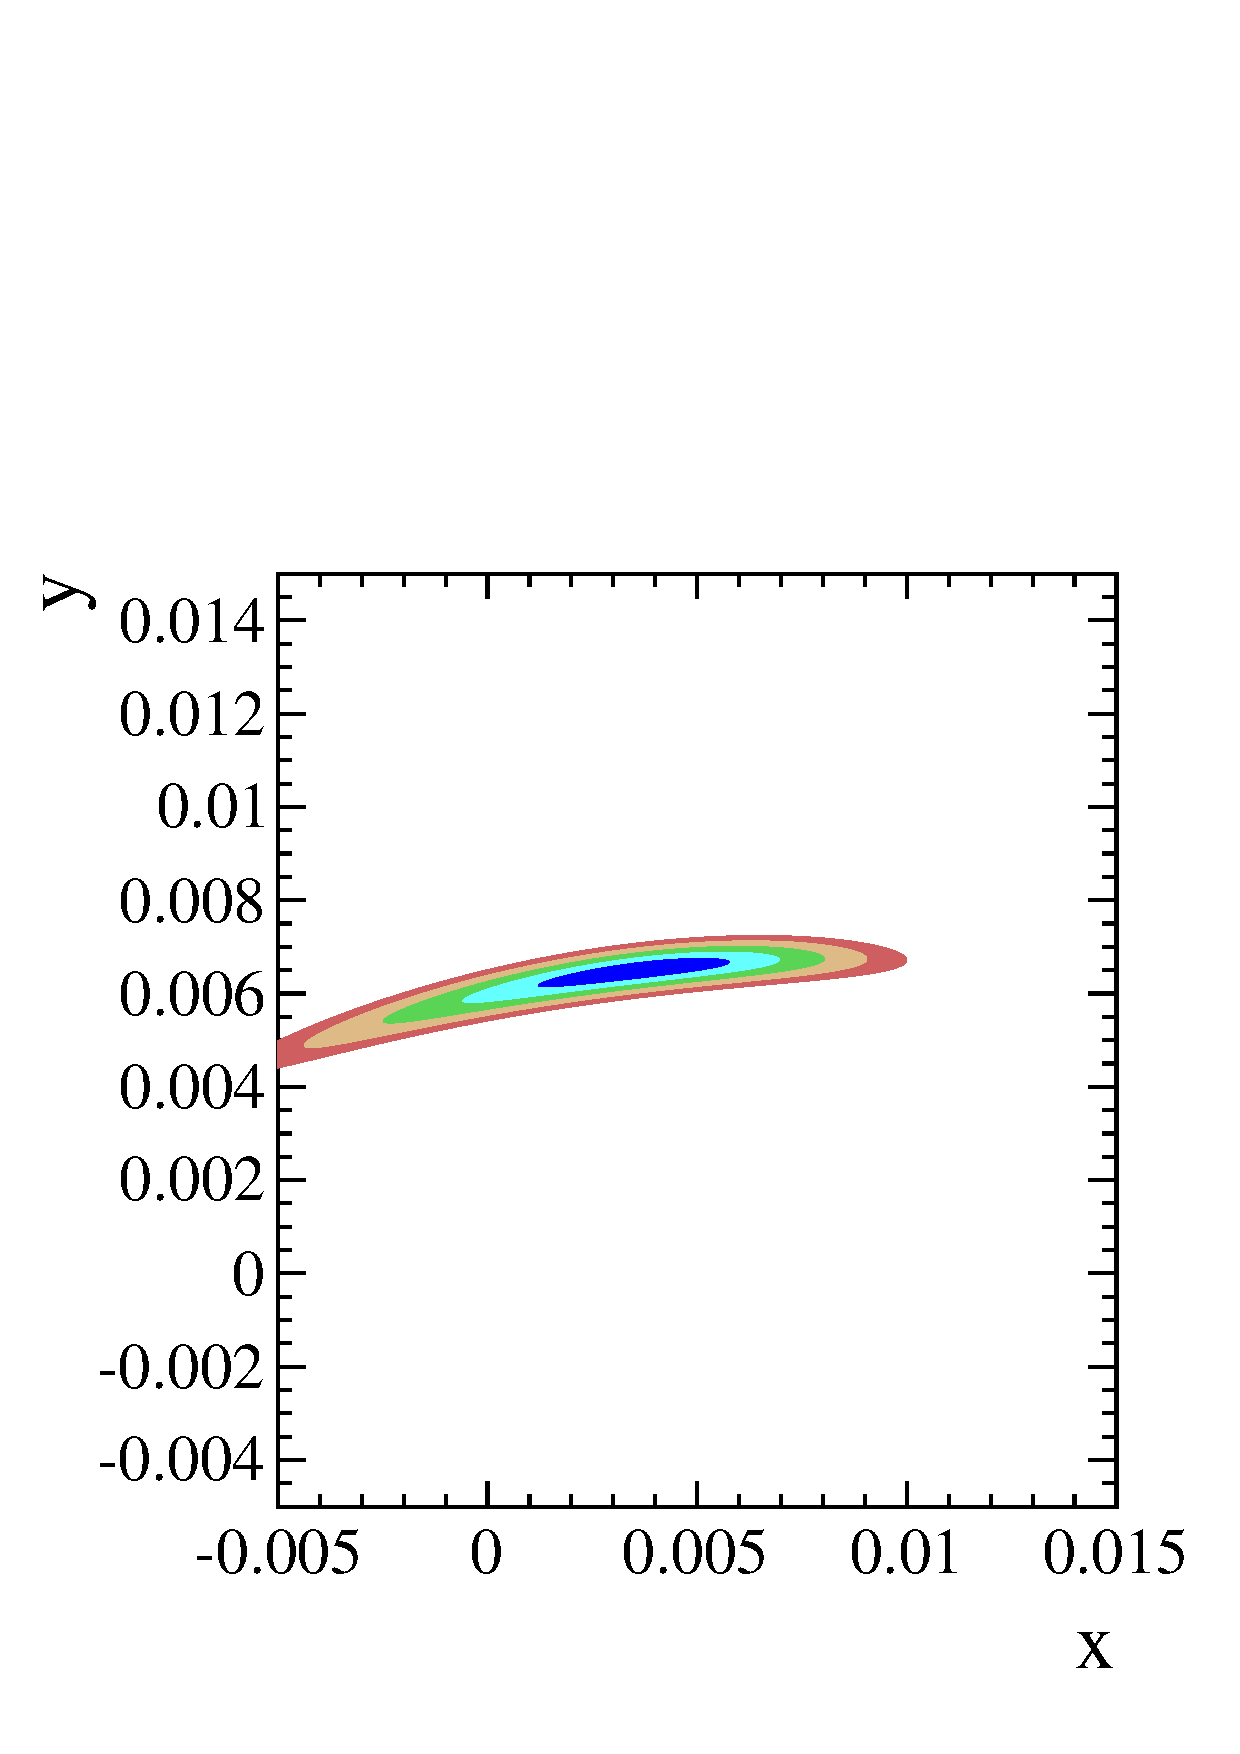
\includegraphics[width=\textwidth]{finalplot_nocpv__graph.pdf}
      \caption{Two dimensional error ellipses for x and y using all measurements listed in Table~\ref{table:nocpv_output_table}.}
      \label{fig:xy_no_cpv_}
    \end{subfigure}%
    \begin{subfigure}[b]{0.4\textwidth}
      \centering
      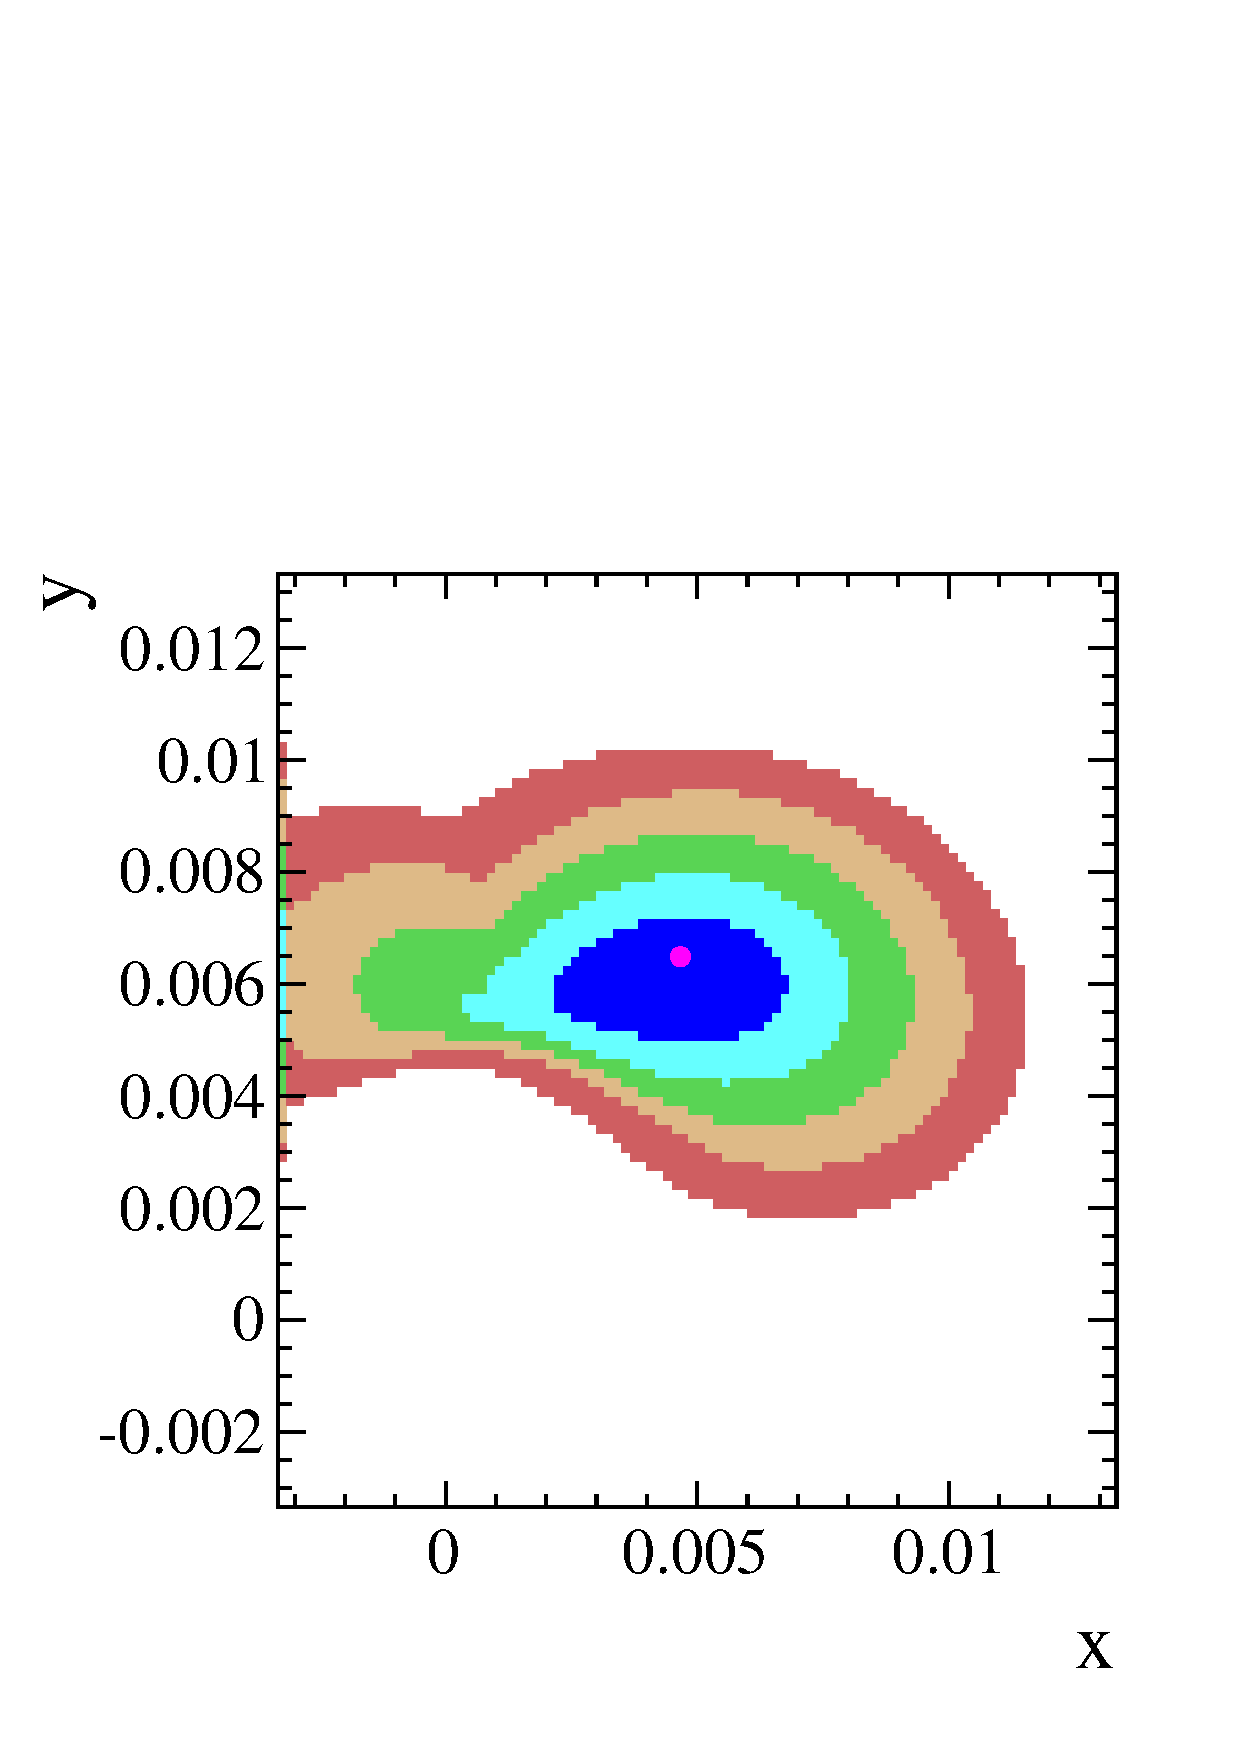
\includegraphics[width=\textwidth]{finalplot_nocpv__babar_graph.pdf}
      \caption{Two dimensional error ellipses for x and y using all available measurements except the .}
      \label{fig:xy_no_cpv_}
    \end{subfigure}%
    %\hspace{2mm}
    
    \begin{subfigure}[b]{0.4\textwidth}
      \centering
      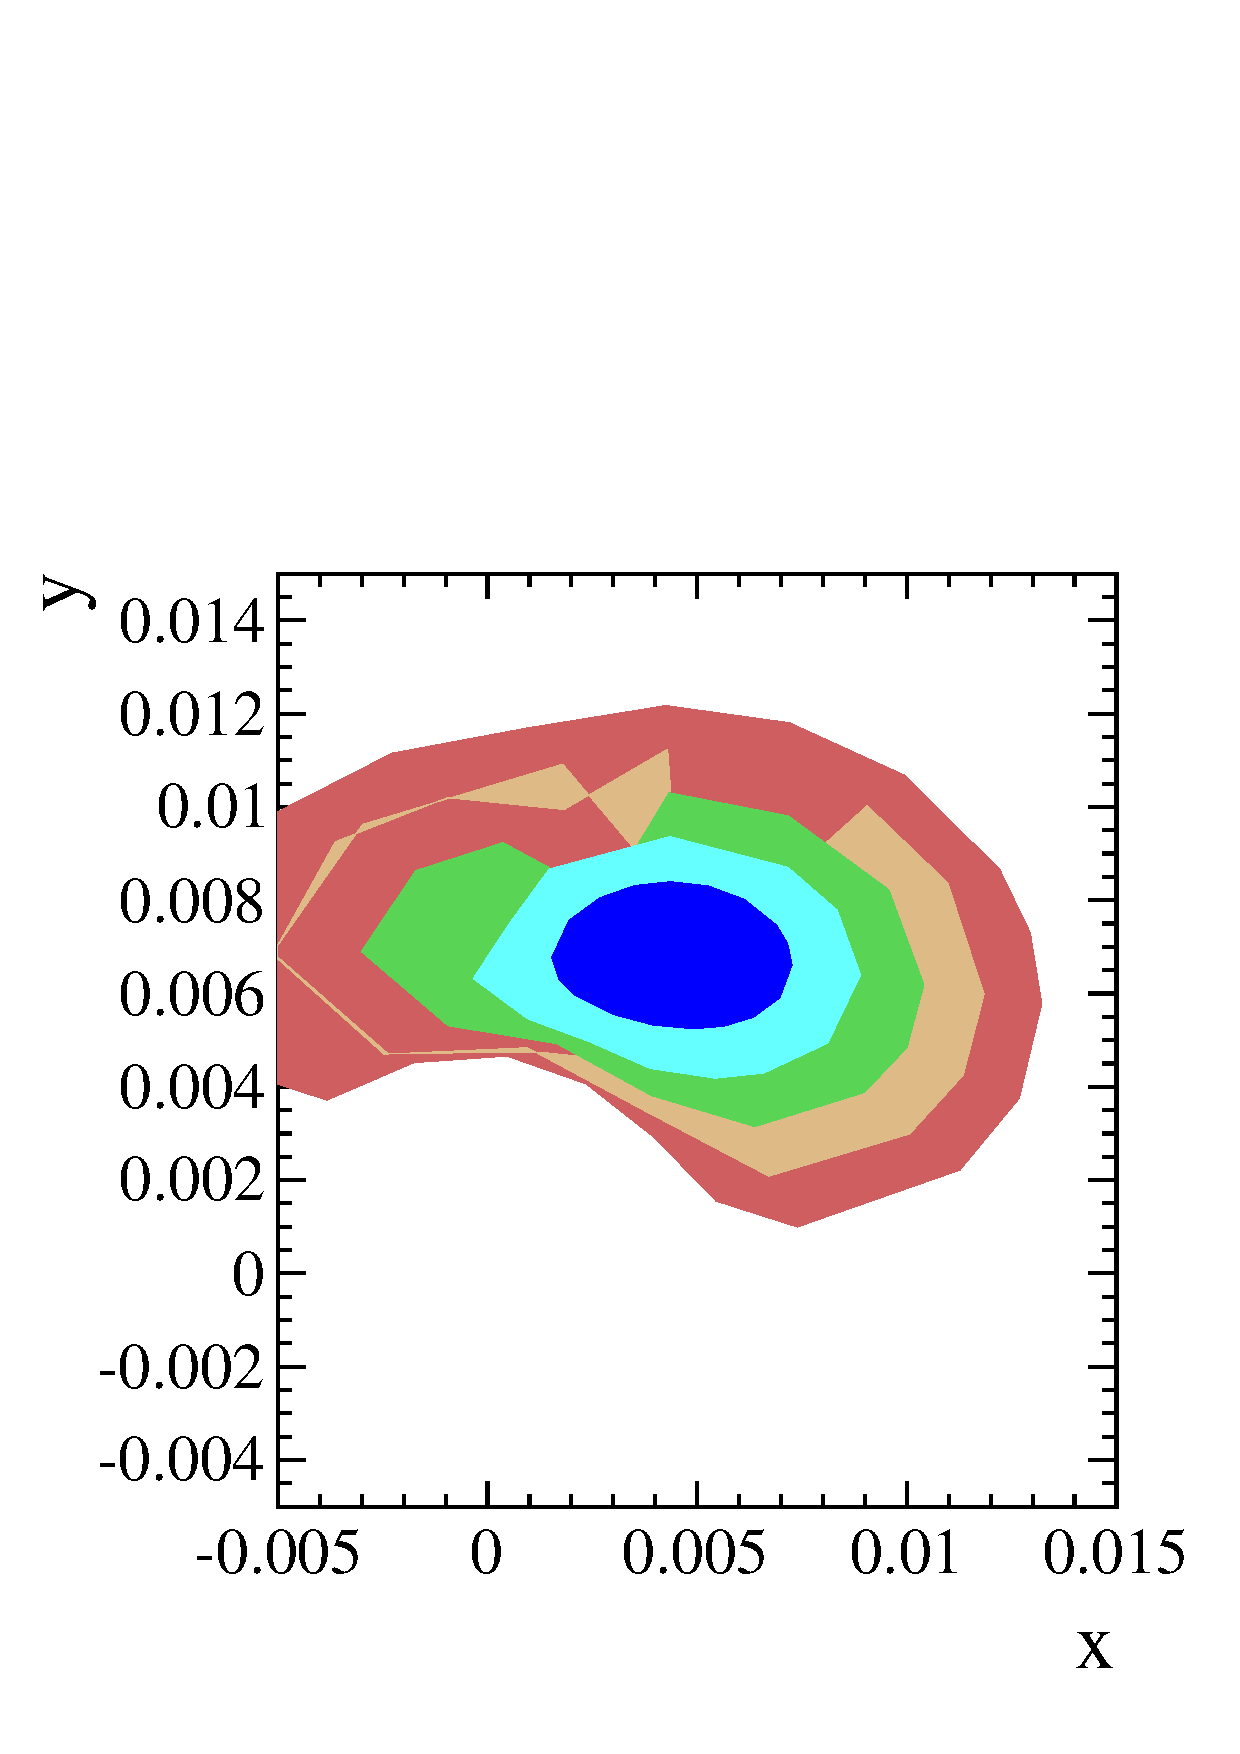
\includegraphics[width=\textwidth]{finalplot_nocpv__belle_babar_graph.pdf}
      \caption{Two dimensional error ellipses for x and y from fit excluding Belle and BaBar $K\pi$ results.}
      \label{fig:xy_no_cpv_nobelle_babar}
    \end{subfigure}%
    \hspace{2mm}
    \begin{subfigure}[b]{0.4\textwidth}
      \centering
      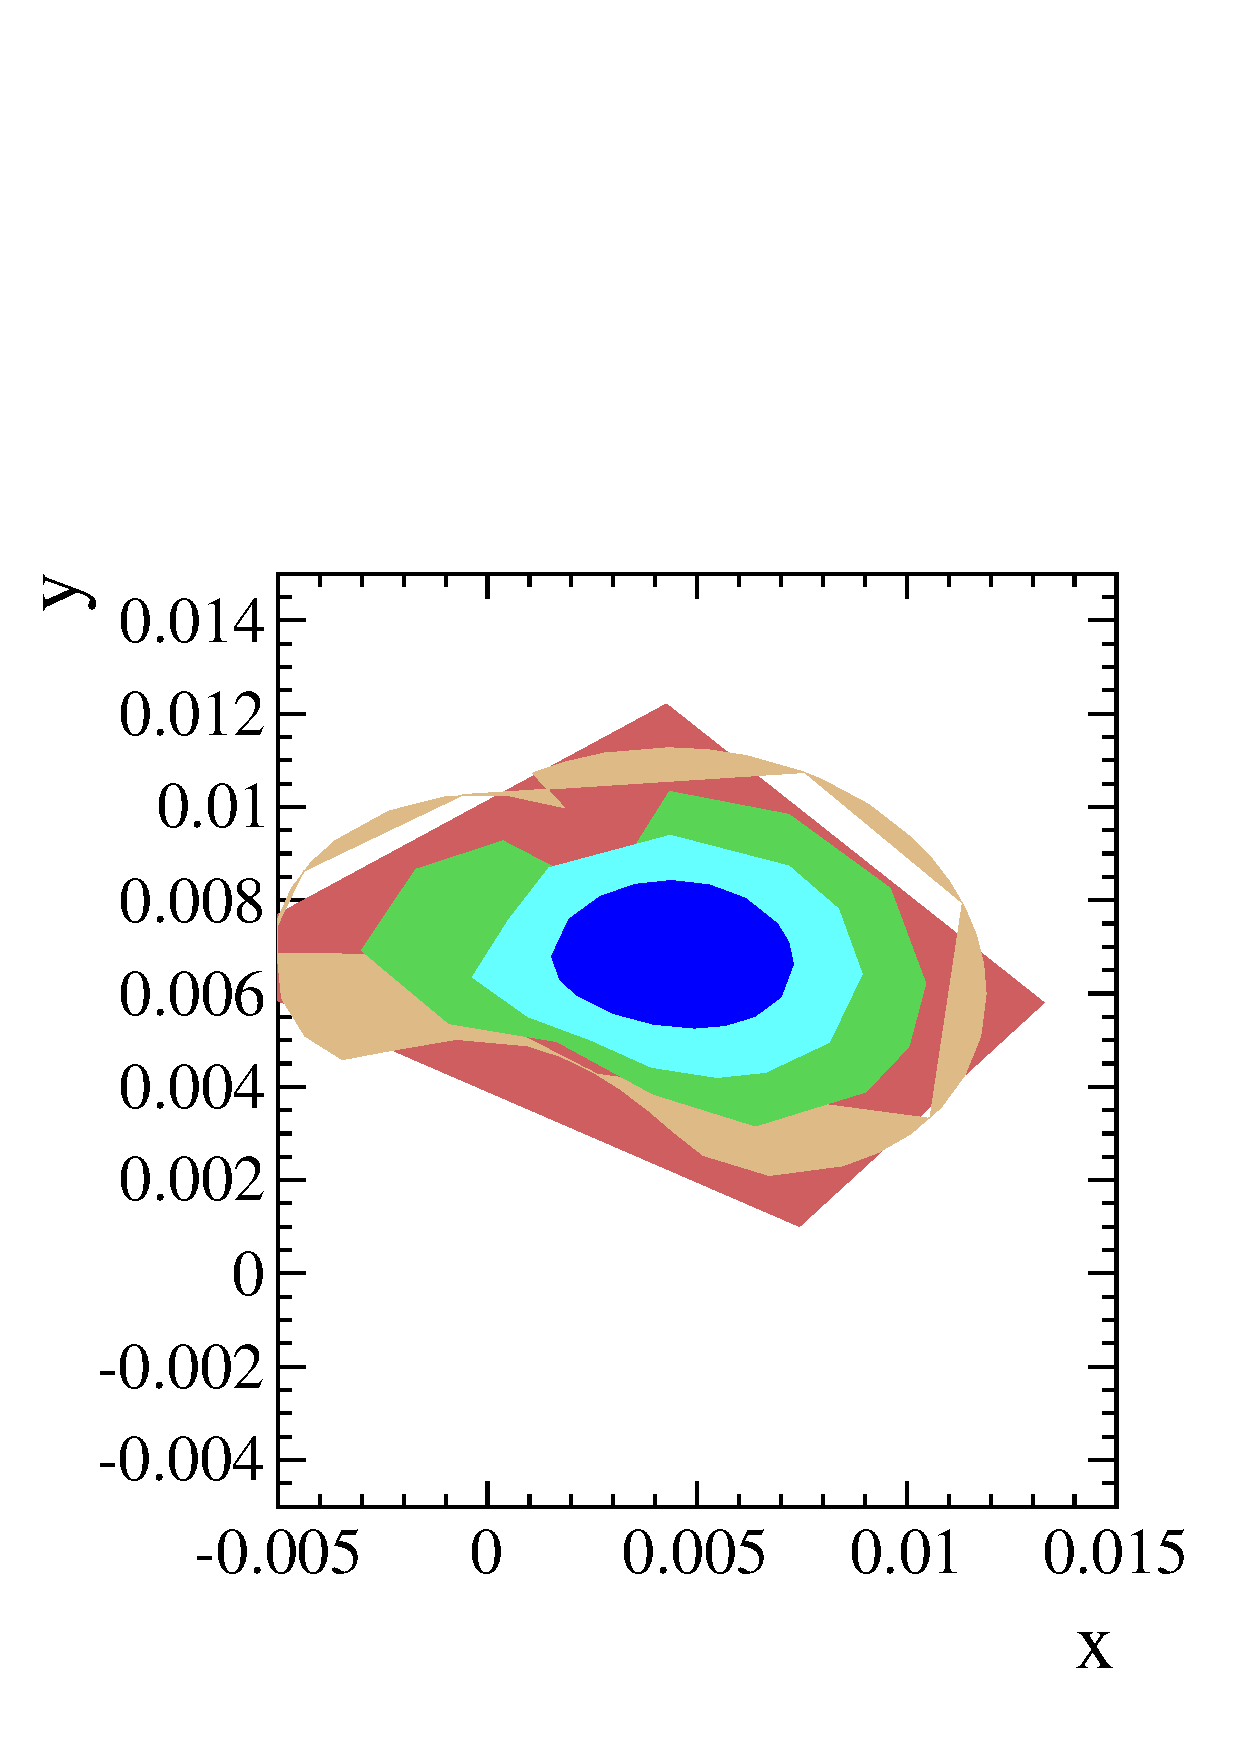
\includegraphics[width=\textwidth]{finalplot_nocpv__belle_babar_cdf_graph.pdf}
      \caption{Two dimensional error ellipses for x and y from fit excluding Belle, BaBar and CDF measurements.}
      \label{fig:xy_no_cpv_nocdf}
    \end{subfigure}%
    %\vspace*{-1.0cm}
  \end{center}
  \caption{Two dimensional error ellipses of $x$ and $y$ from fit for No CPV. Exclusion of the Belle and BaBar results drastically change the slope of the error ellipses. The differing colors represent the 1-5$\sigma$ contours.}
  \label{fig:xy_nocpv_variations}
\end{figure}
\subsection{No Direct CP Violation Allowed}
Table~\ref{table:nodcpv_output_table} lists the results of the global fit of no direct
CP violation. The final three columns of the table represent the effect of the 
inclusion of the preliminary LHCb $A_\Gamma$ result in the global fit.
The inlcusion of this result does not change the central values or errors substantially.


\begin{table}[htdp]
%\begin{tiny}

\begin{center}
\resizebox{16cm}{!} {
\begin{tabular}{|c||c||c||c||c|}
\hline
& All Measurements & No Belle, BaBar$K\pi$& No Belle, BaBar$K\pi$, add $A_{\Gamma\text{ LHCb}}$ & No Belle, BaBar, CDF $K\pi$, add $A_{\Gamma\text{ LHCb}}$ \\ \hline

$x(\times10^{-3})$ & $ 5.191\pm 1.746 $& $4.843\pm 1.782$& $4.845\pm1.782$& $4.844\pm1.787$ \\ \hline

$y(\times10^{-3})$ &$ 6.343\pm 0.905$ & $6.797\pm 1.029$& $6.797\pm 1.030$& $6.809\pm 1.031$ \\ \hline

$\delta_{K\pi}(\times10^{-1})[\text{rad}]$ &$2.468\pm 1.763$ & $3.187\pm 2.021$&$3.188\pm 2.021$ & $3.084\pm 2.040$ \\ \hline

$R_D(\times10^{-3})$ & $ 3.571\pm 0.046 $&$3.555\pm0.046$ & $3.556\pm 0.046$& $3.556\pm 0.047$ \\ \hline

$|q/p|(\times10^{-1})$ & $9.931 \pm 0.125$& $9.935\pm0.135$& $9.929\pm 0.131$ & $9.930\pm0.130 $\\ \hline

$\chi^2/ndf$ & 24.8569/28 & 19.0559/13& 19.3925/15& 8.61793/12\\ \hline

\end{tabular}
}
\end{center}
\caption{Output values of No Direct CPV allowed global fit. Different columns list 
subsets of allowed data.}
\label{table:nodcpv_output_table}
%\end{tiny}
\end{table}%



\begin{figure}[htb]
  \begin{center}
    \begin{subfigure}[b]{0.4\textwidth}
      \centering
      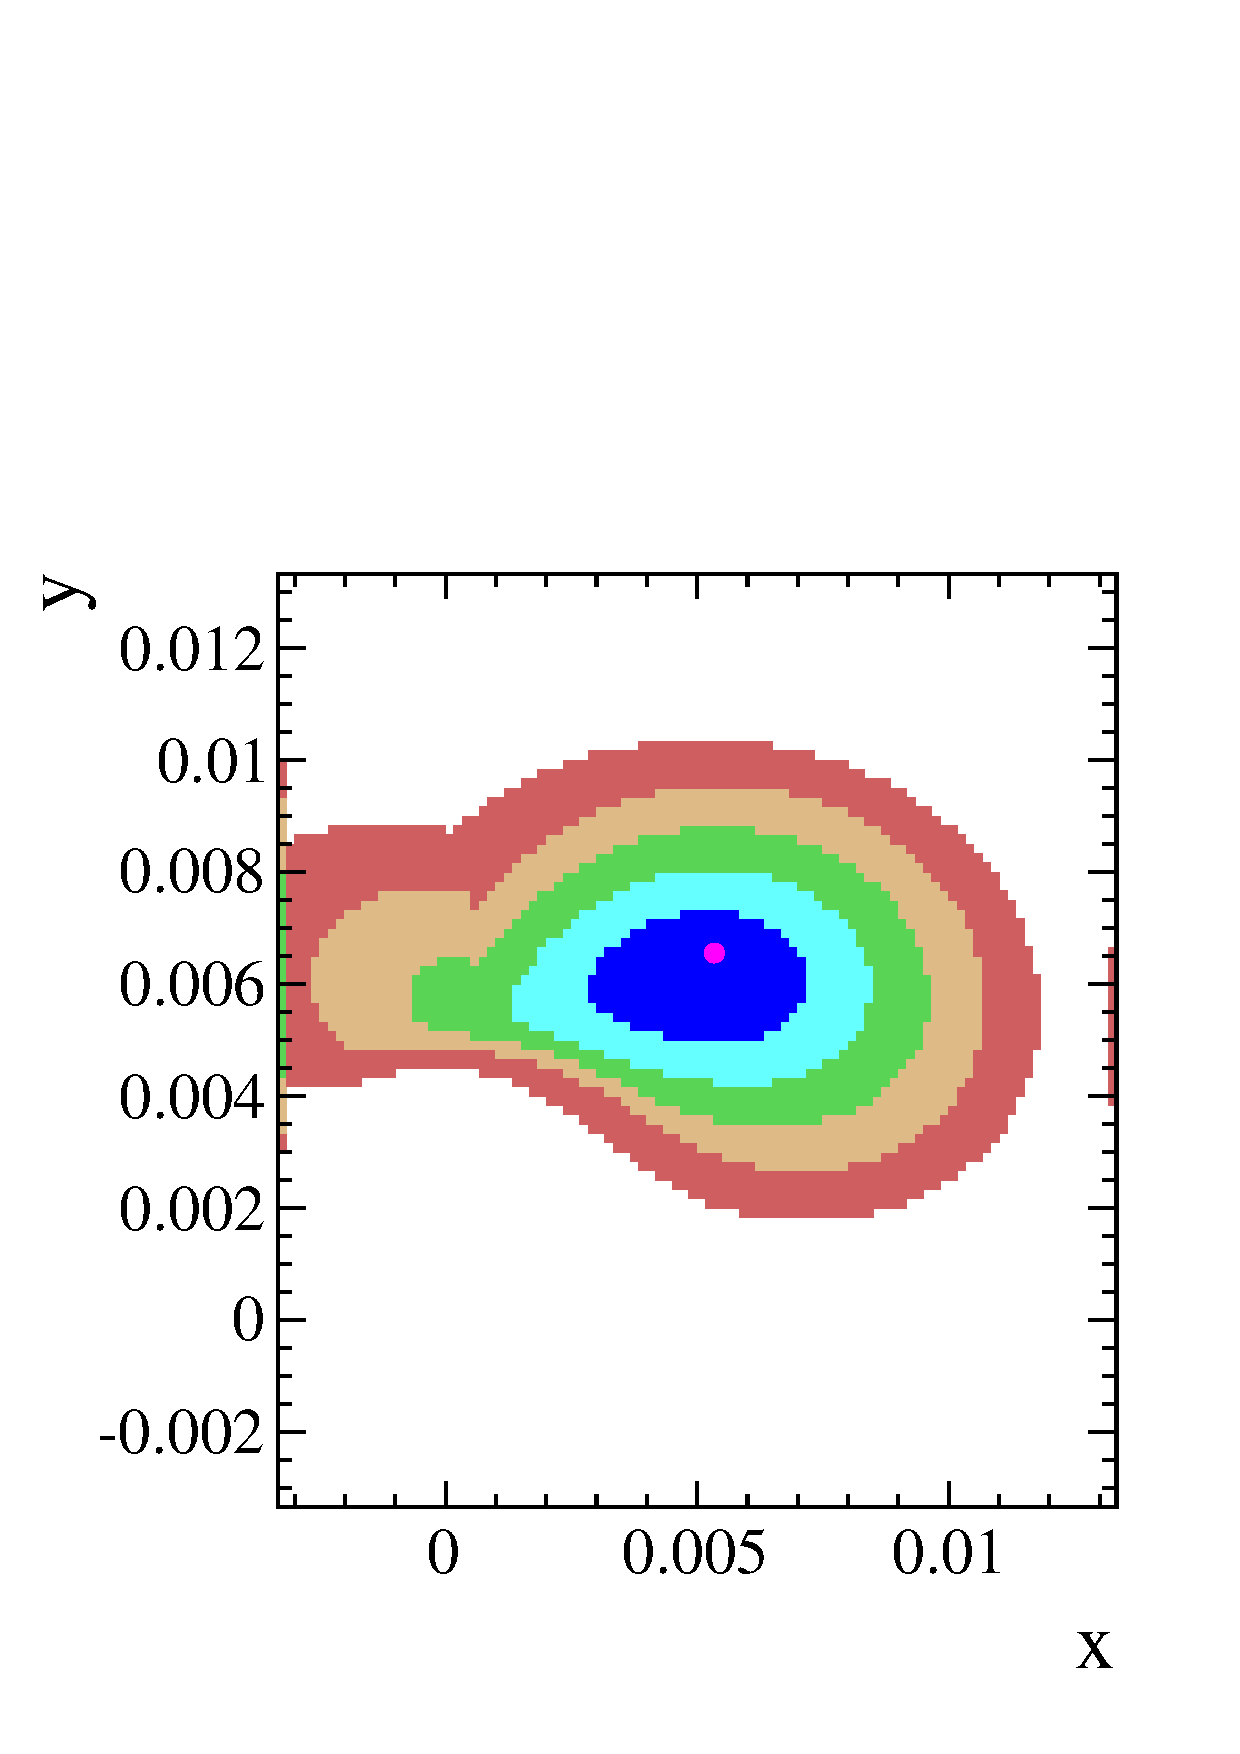
\includegraphics[width=\textwidth]{finalplot_nodcpv__.pdf}
      \caption{Two dimensional error ellipses for x and y from fit to all listed data.}
      \label{fig:all_nodcpv}
    \end{subfigure}%
    \hspace{2mm}
    \begin{subfigure}[b]{0.4\textwidth}
      \centering
      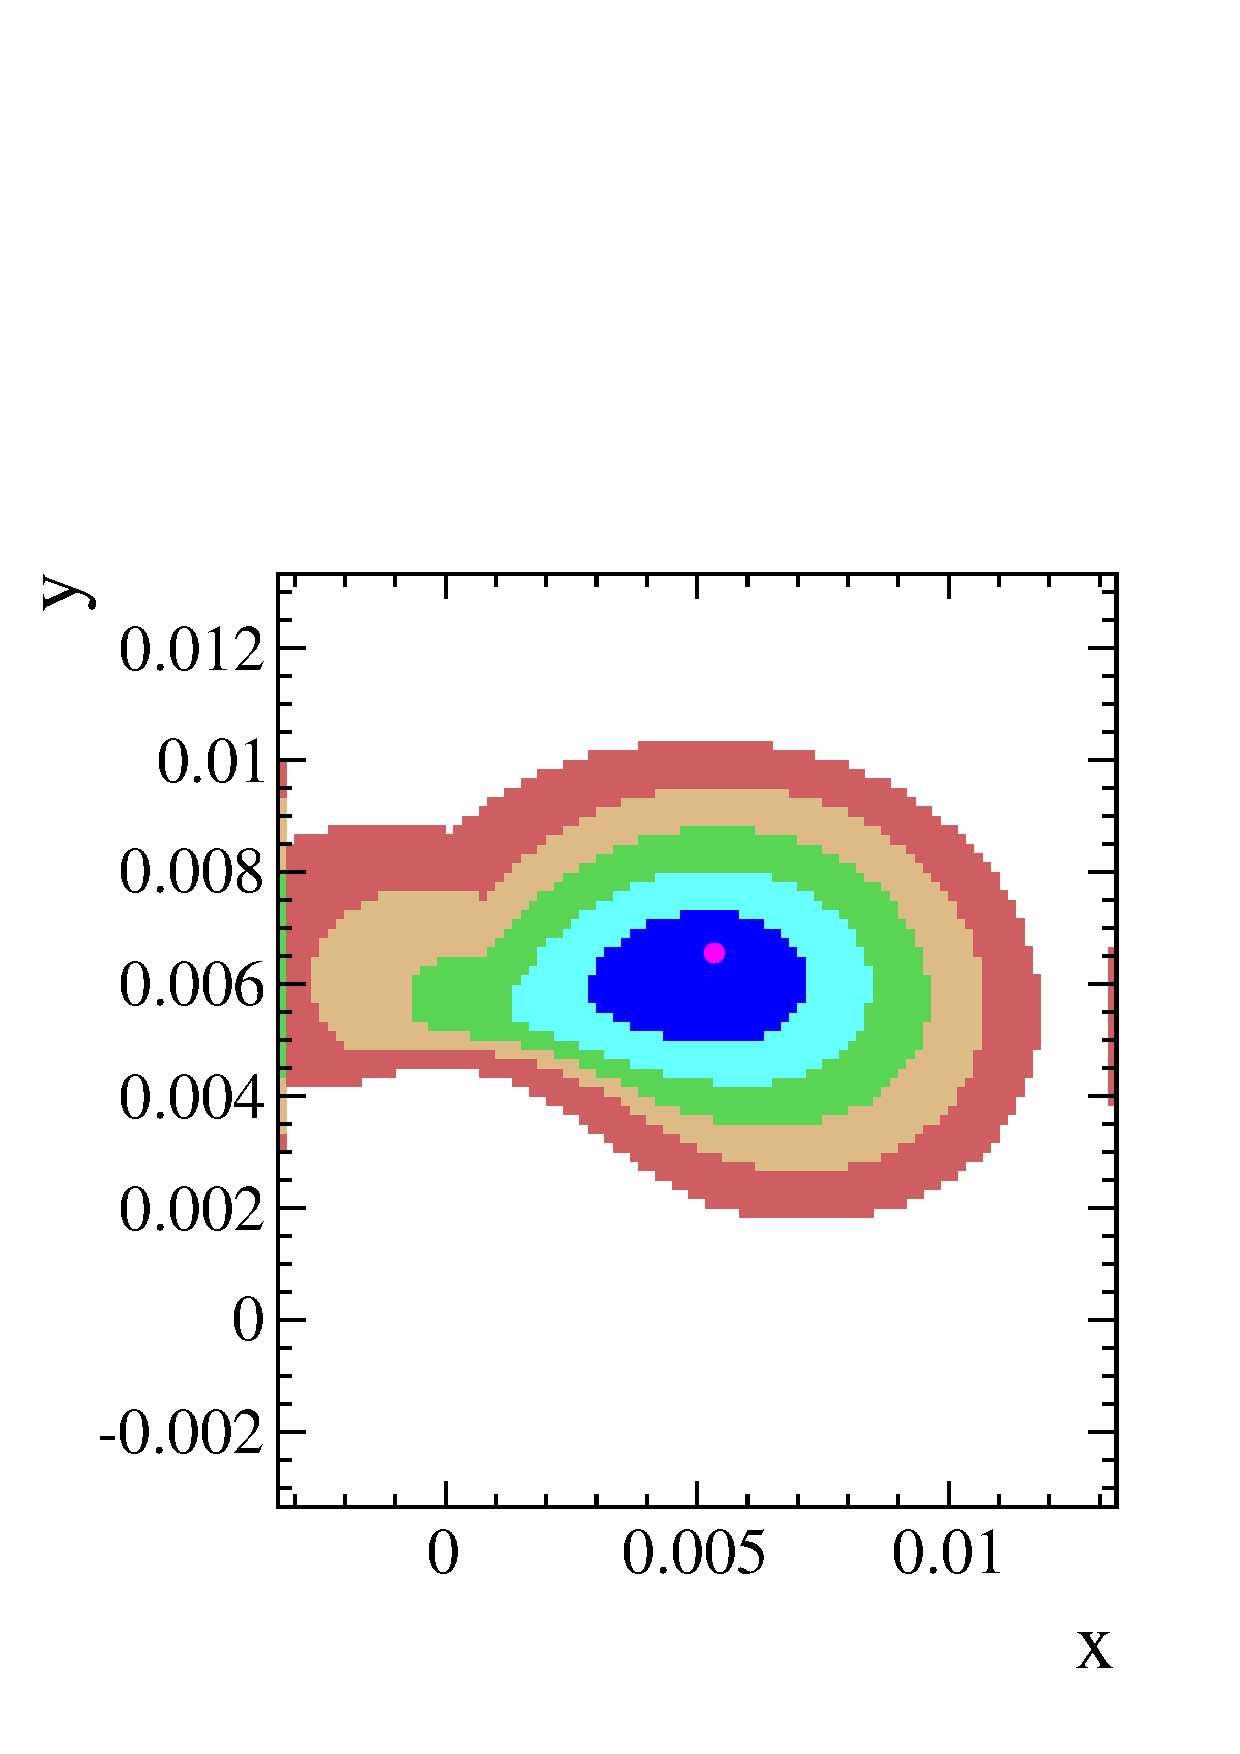
\includegraphics[width=\textwidth]{finalplot_nodcpv___hfag_agamma.pdf}
      \caption{Two dimensional error ellipses for x and y from fit to all data except LHCb $A_\Gamma$.}
      \label{fig:all_nodcpv_no_lhcb_agamma}
    \end{subfigure}%
    \\
%%%%%%%%%
    %\hspace{2mm}
    \begin{subfigure}[b]{0.4\textwidth}
      \centering
      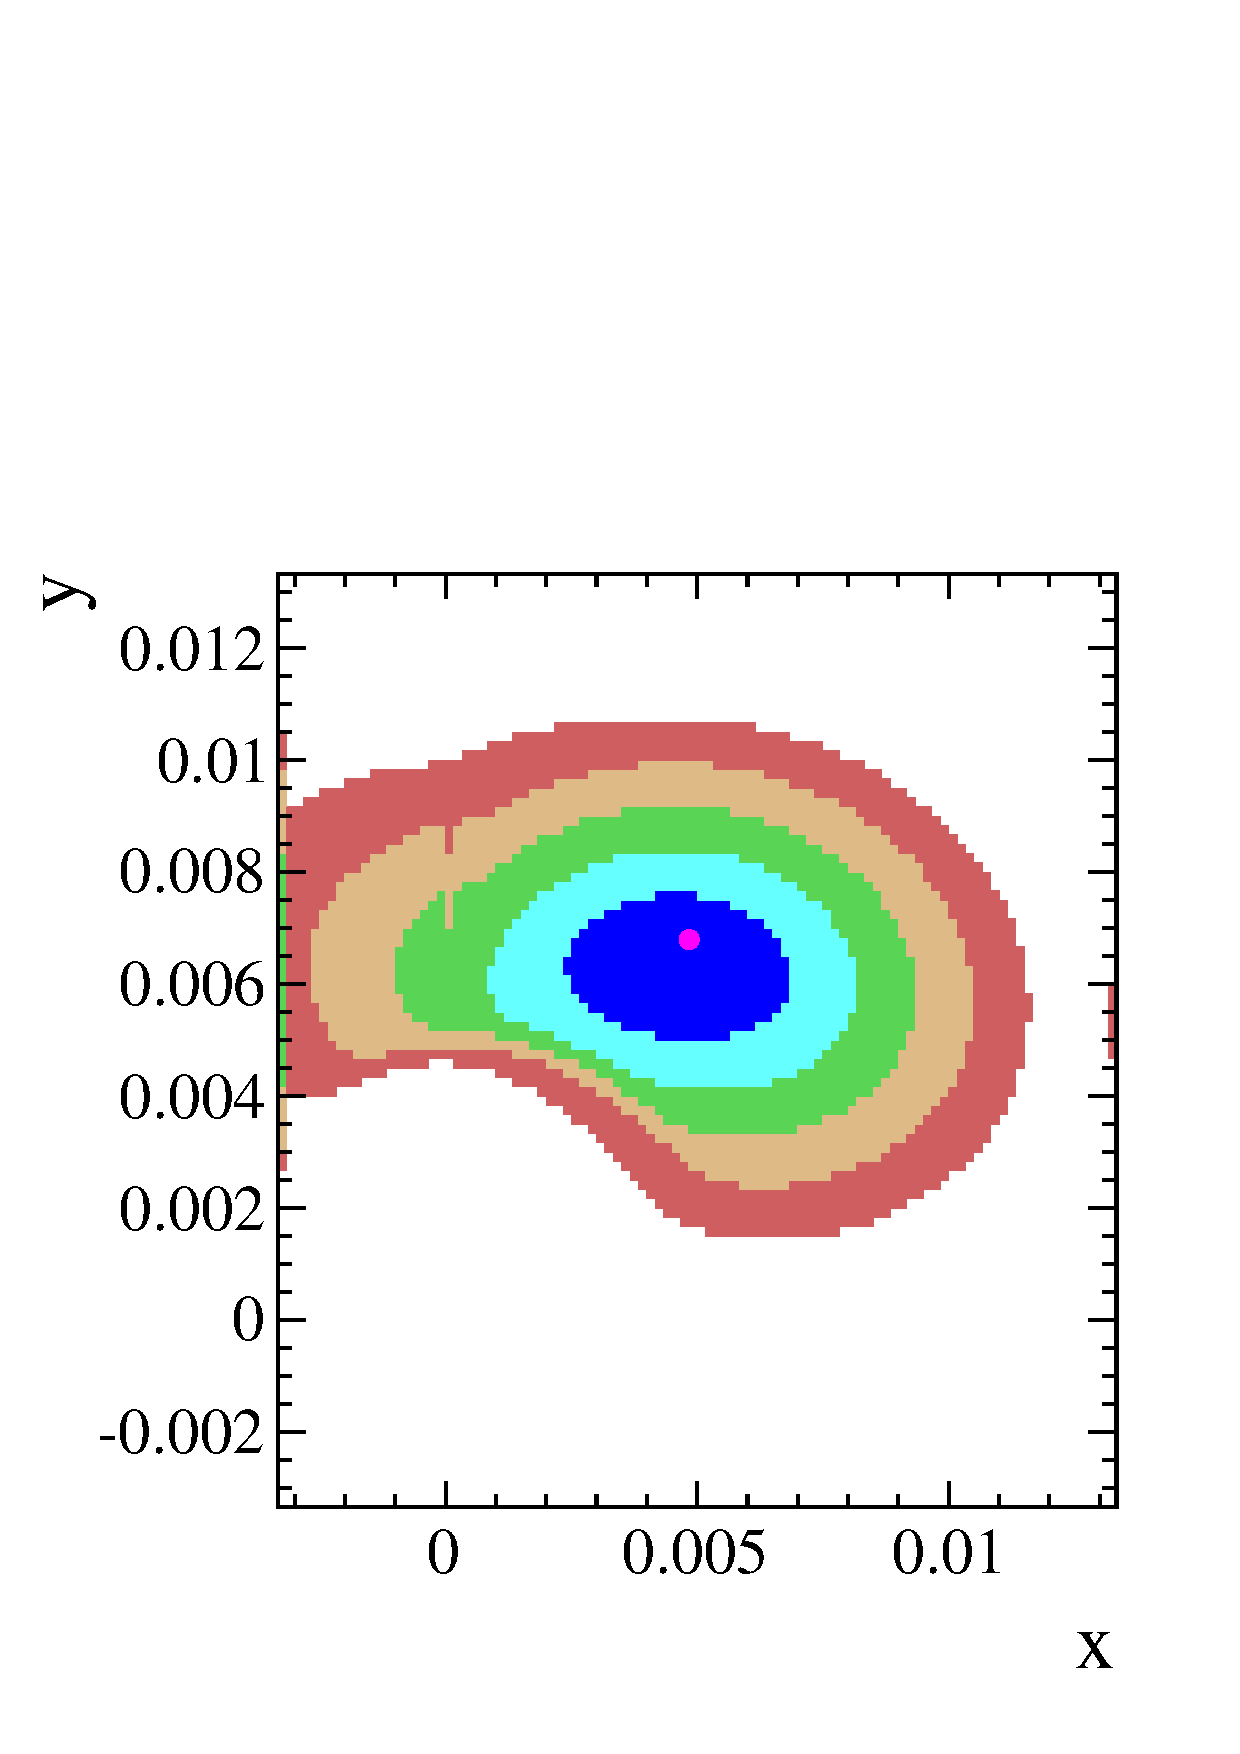
\includegraphics[width=\textwidth]{finalplot_nodcpv__nobelle_babar_.pdf}
      \caption{x vs y for Data excluding Belle and Babar $K \pi$ results.}
      \label{fig:nodcpv_no_belle_babar}
    \end{subfigure}%
    \hspace{2mm}
    \begin{subfigure}[b]{0.4\textwidth}
      \centering
      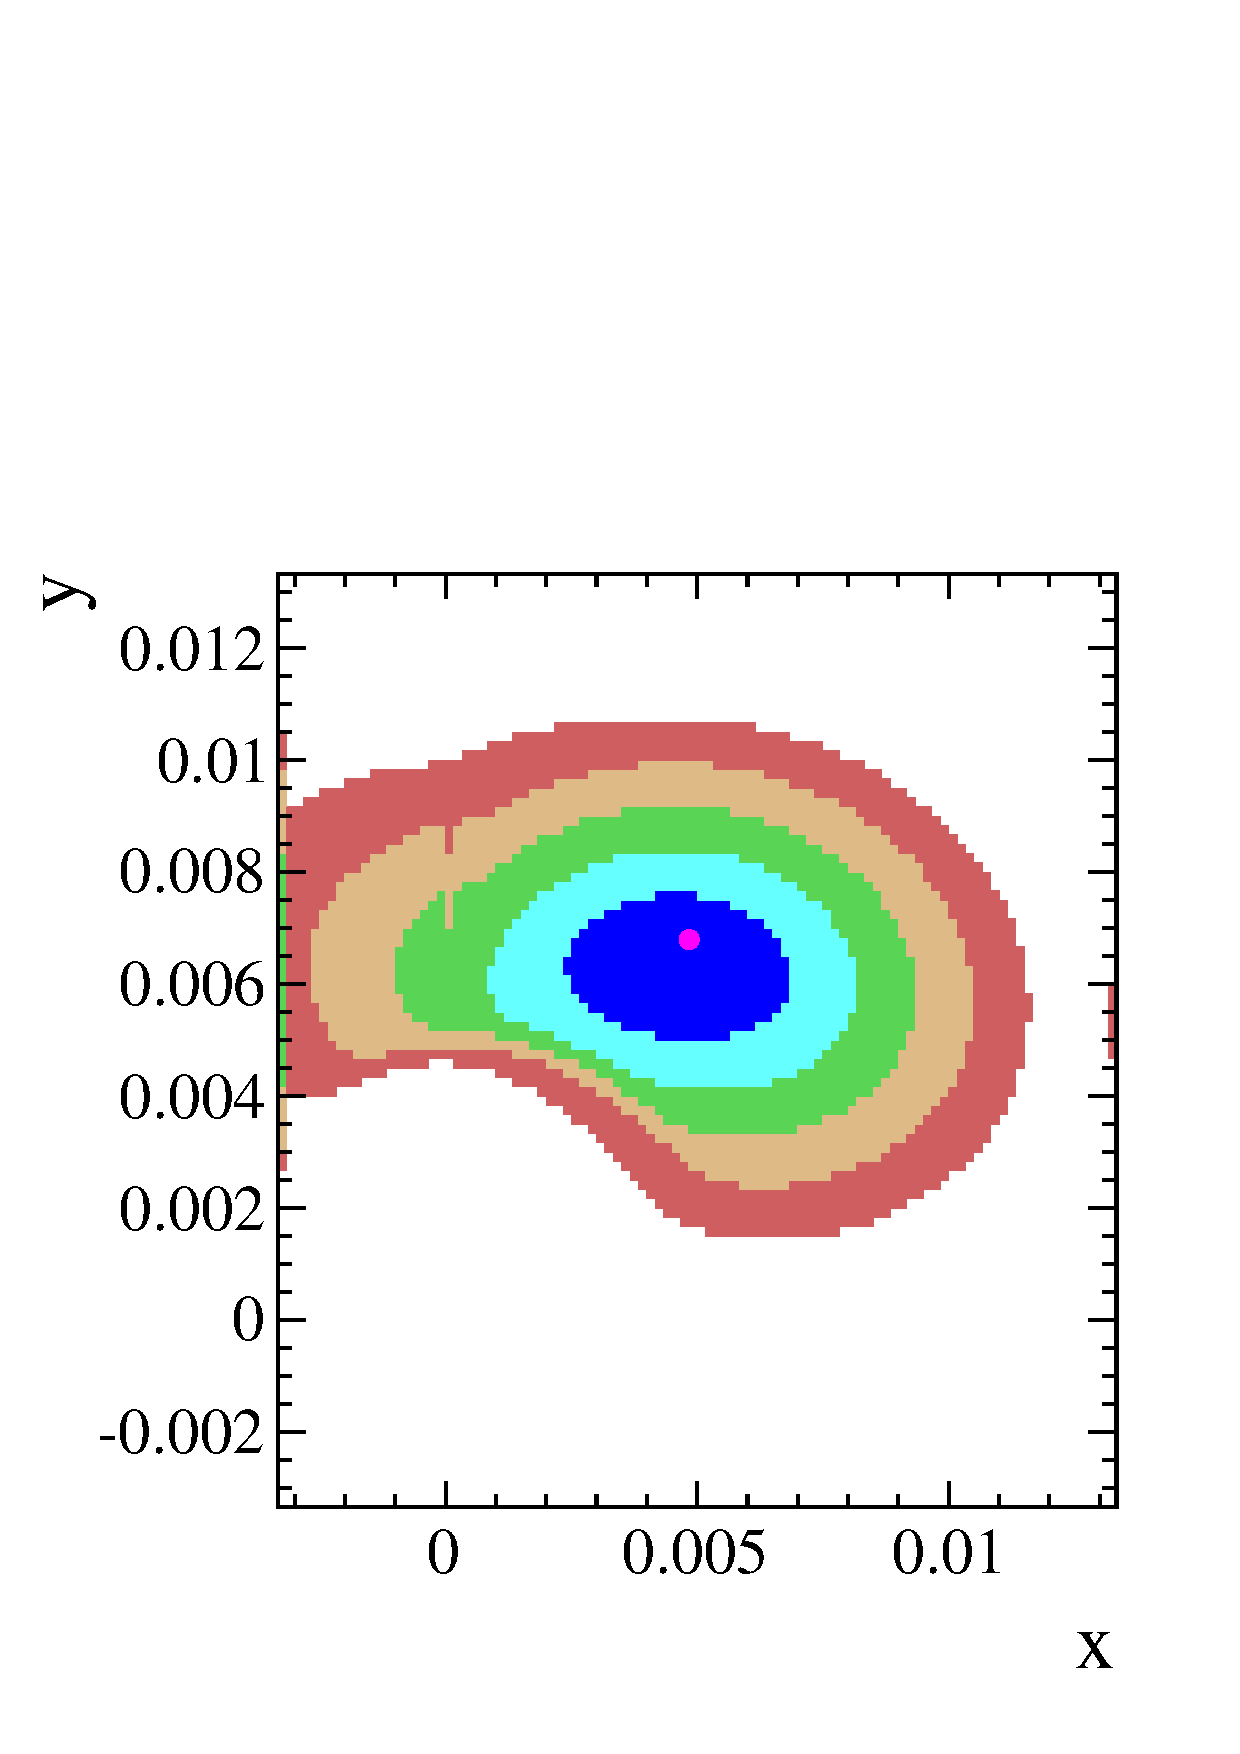
\includegraphics[width=\textwidth]{finalplot_nodcpv__nobelle_babar__hfag_agamma.pdf}
      \caption{Two dimensional error ellipses for x and y for No Direct CPV, excluding Belle and BaBar $K\pi$ results, and excluding LHCb $A_\Gamma$.}
      \label{fig:nodcpv_no_belle_babar_no_lhcb_agamma}
    \end{subfigure}%
    %\vspace*{-1.0cm}
  \end{center}
  \caption{Two dimensional error ellipses of fit for All CPV including differing sets of data for $x$ vs $y$. The biggest differences come from including the CDF result, which elongates the error ellipses. The differing colors represent the 1-5$\sigma$ contours.}
  \label{fig:xy_nodcpv_variations}
\end{figure}


%%%%%%%%%%%%%%%%%%%%%%%%%%%%%%%%%%%%%%%%%%%%
\subsection{All CP Violation Allowed}
Table~\ref{table:allcpv_output_table} lists the results of the global All CP Violation
allowed fit. Again, the latter columns list the differing subsets of the data to explore
the variation in global $\chi^2/$ndf. The most noticable difference between all fits
is the evaluation of $x$, which varies quite a bit with the inclusion of differing datasets.


%%%%%%%%%%%%%%% XY %%%%%%%%%%%%%%%%%%%%%%%%%
%\begin{table}[htdp]
%\begin{tiny}

\begin{center}
\resizebox{16cm}{!} {
\begin{tabular}{|c||c||c||c||c|}
\hline
& All Measurements & No Belle, BaBar& No Belle, BaBar, $A_{\Gamma\text{ LHCb}}$ & No Belle, BaBar, CDF,$A_{\Gamma\text{ LHCb}}$ \\ \hline

$x(\times10^{-3})$& $3.737\pm 1.630$ &$4.817\pm1.688$ &$4.772\pm1.685$ &$4.601\pm1.664$ \\ \hline

$y(\times10^{-3})$& $6.128 \pm 0.743$ & $6.868\pm 0.984$&$6.908\pm0.963$ & $6.956\pm0.867$\\ \hline

$\delta_{K\pi}(\times10^{-1})[\text{rad}]$& $ 1.146\pm 2.127$ & $3.246\pm1.935$& $3.329\pm1.891$& $3.250\pm1.756$\\ \hline

$\phi(\times10^{-1})[\text{rad}]$& $-0.642\pm1.255 $ &$-0.623\pm 1.055$&$-0.651\pm1.046$ & $-1.534\pm1.712$\\ \hline

$R_D^-(\times10^{-3})$& $3.501 \pm 0.040$&$3.568\pm 0.049$& $3.567\pm0.049$&$3.582\pm0.055$ \\ \hline

$R_D^+(\times10^{-3})$& $3.496\pm 0.036$ & $3.547\pm 0.044$ & $3.548\pm 0.043$&$3.533\pm0.046$ \\ \hline

$|q/p|(\times10^{-1})$& $9.631\pm 0.693$& $9.513\pm0.823$&$9.474\pm0.800$ & $8.880\pm1.082$\\ \hline

$\chi^2/ndf$& 59.9402/29 &18.8317/11 & 19.1817/14 & 7.72181/9\\ \hline

\end{tabular}
}
\end{center}
\caption{Output of the All CP Violation allowed global fit. Different Columns list 
differing subsets of data included in the fit.}
\label{table:allcpv_output_table}
%\end{tiny}
\end{table}%

%\begin{figure}[htb]
%  \begin{center}
%    \begin{subfigure}[b]{0.4\textwidth}
%      \centering
%      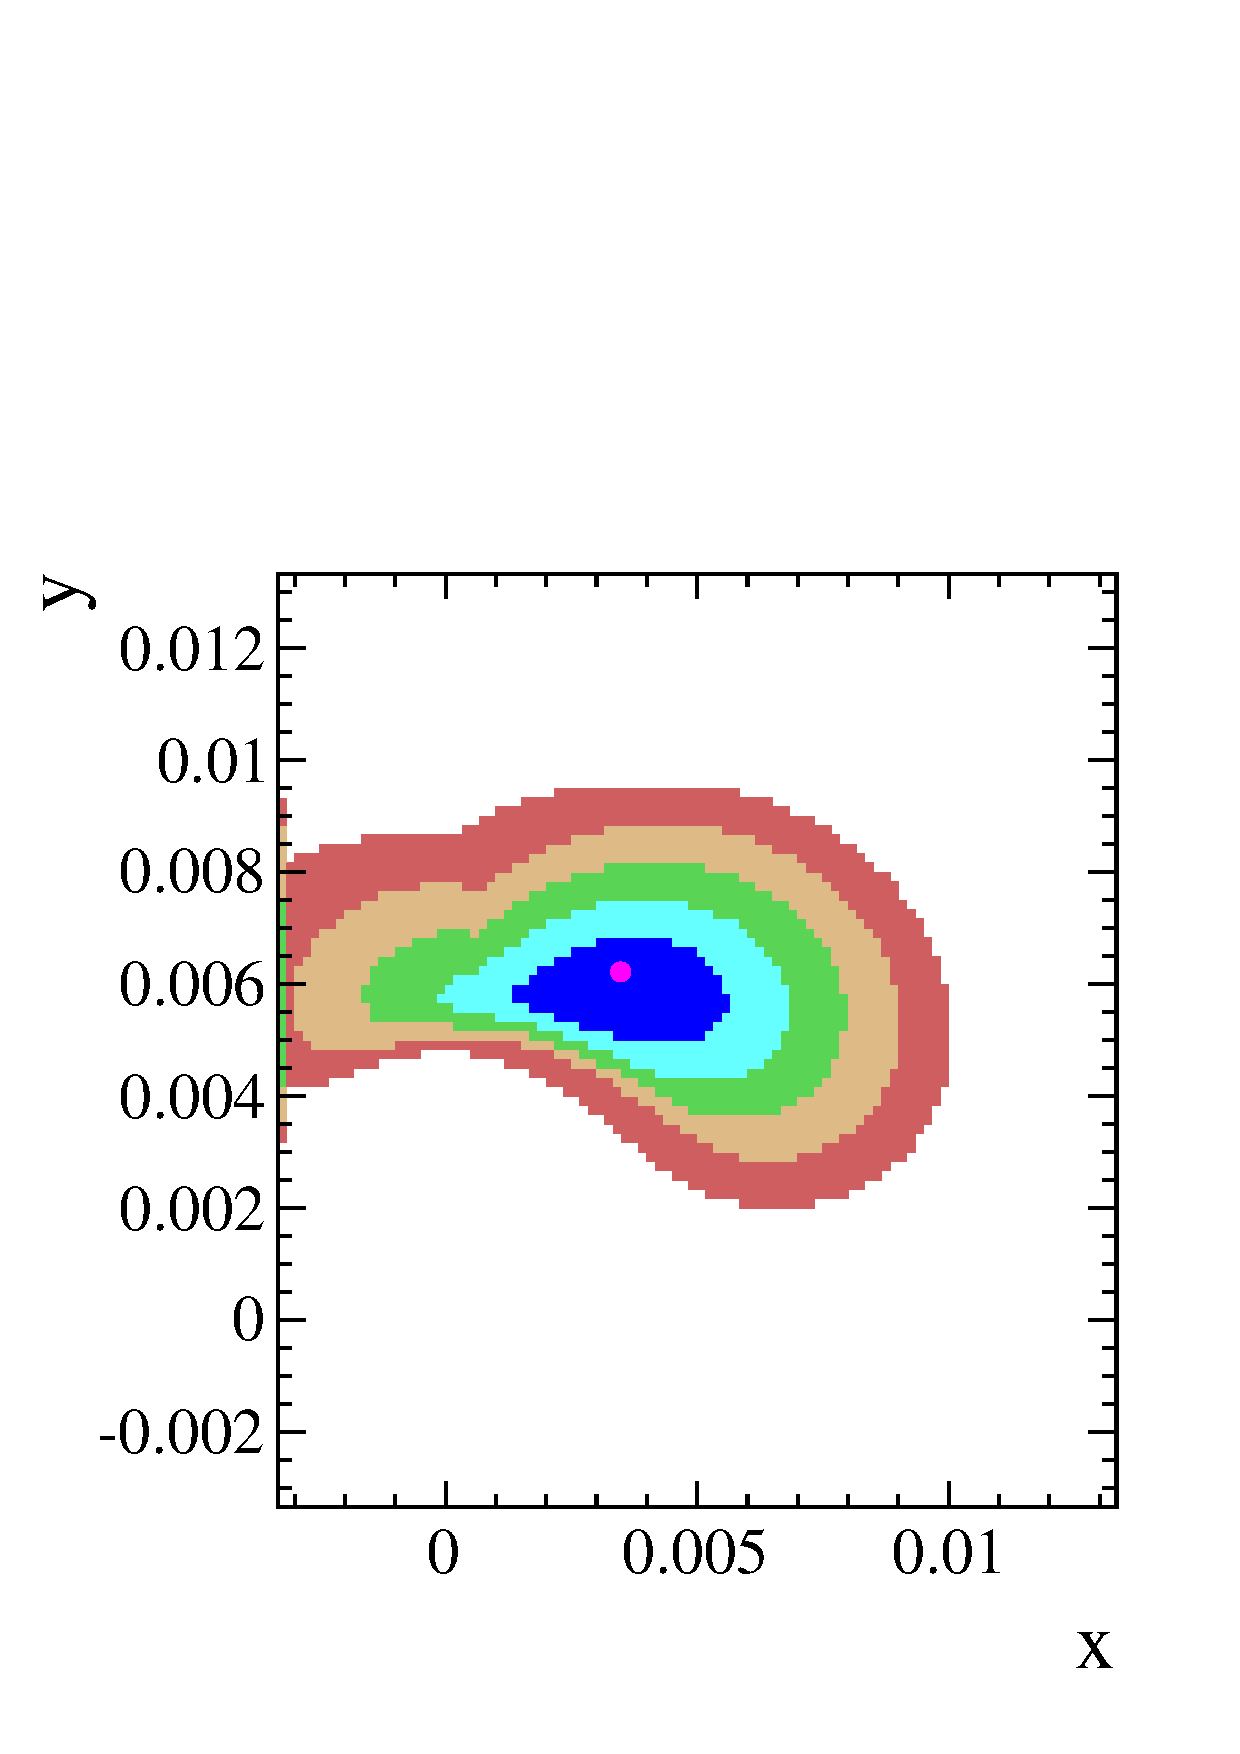
\includegraphics[width=\textwidth]{finalplot_allcpv_no_belle_babar_graph_hfag_agamma.pdf}
%      \caption{Two dimensional error ellipses for x and y from fit excluding Belle and BaBar $K\pi$ results. Does not include latest $A_\Gamma$ result of LHCb.}
%      \label{fig:xy_all_cpv_no_agamma}
%    \end{subfigure}%
%    \hspace{2mm}
%    \begin{subfigure}[b]{0.4\textwidth}
%      \centering
%      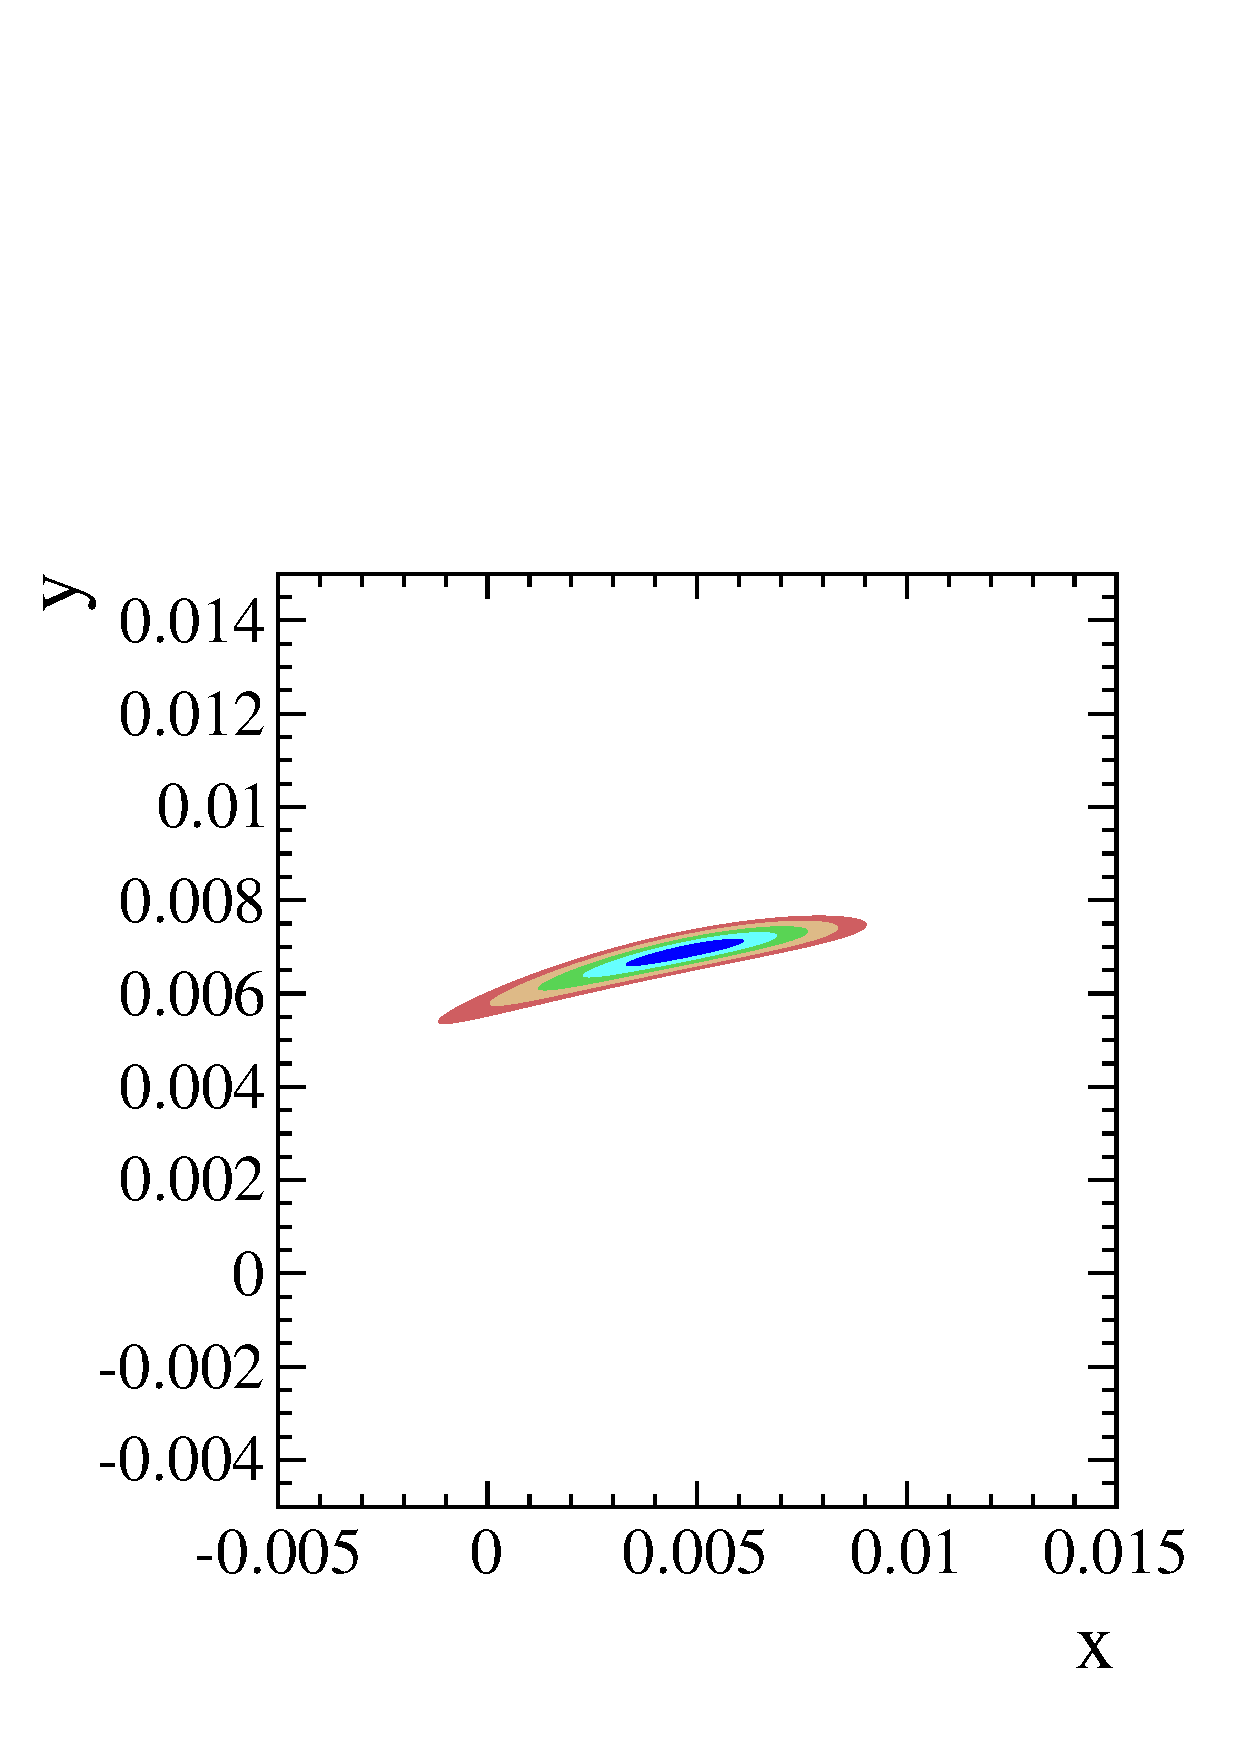
\includegraphics[width=\textwidth]{finalplot_allcpv_no_belle_babar_graph_lhcb_agamma.pdf}
%      \caption{Two dimensional error ellipses for x and y from fit excluding Belle and BaBar $K\pi$ results. Include latest $A_\Gamma$ result of LHCb.}
%      \label{fig:xy_all_cpv_with_agamma}
%    \end{subfigure}%
%    \\
%%%%%%%%%%
%    %\hspace{2mm}
%    \begin{subfigure}[b]{0.4\textwidth}
%      \centering
%      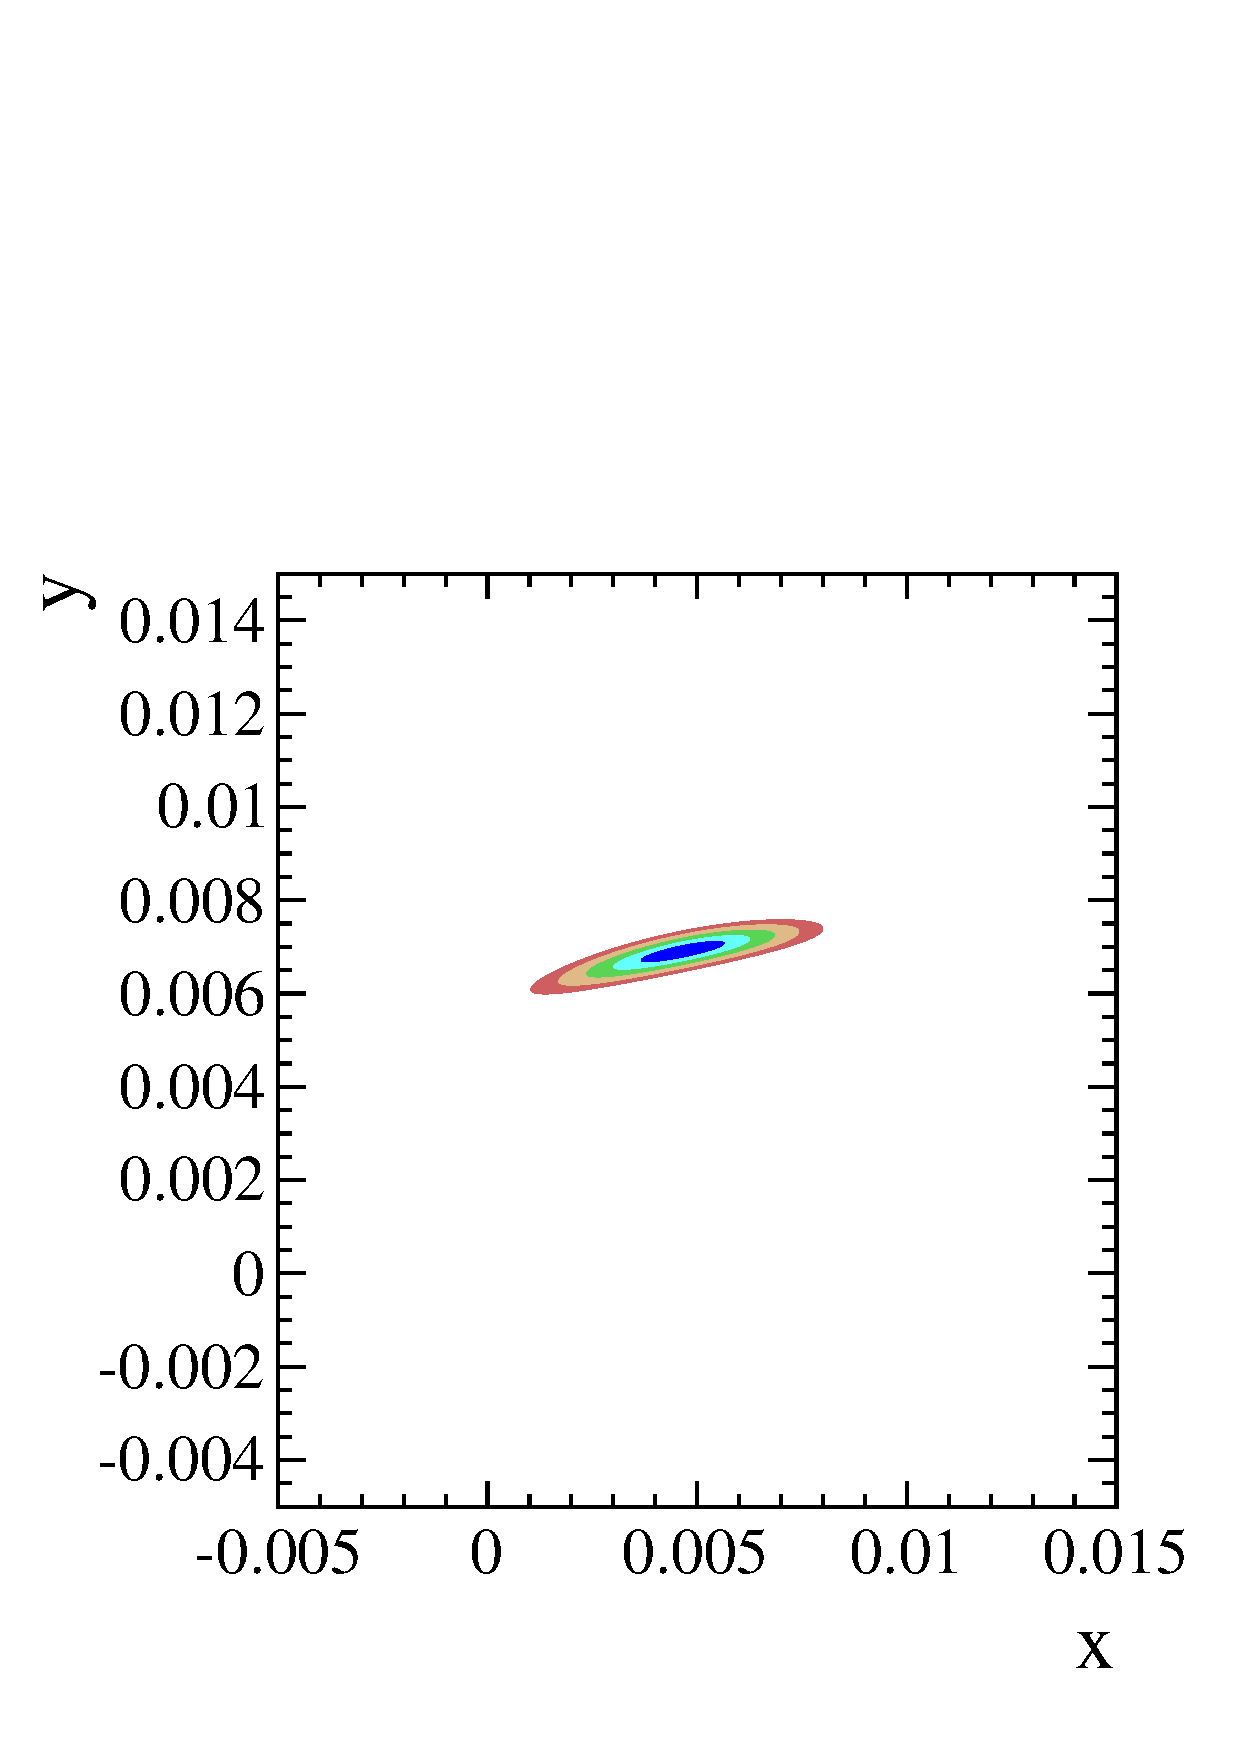
\includegraphics[width=\textwidth]{finalplot_allcpv_no_belle_babar_cdf_graph_hfag_agamma.pdf}
%      \caption{Two dimensional error ellipses for x and y from fit excluding Belle, BaBar and CDF $K\pi$ results. Does not include latest $A_\Gamma$ result of LHCb.}
%      \label{fig:xy_all_cpv_no_agamma}
%    \end{subfigure}%
%    \hspace{2mm}
%    \begin{subfigure}[b]{0.4\textwidth}
%      \centering
%      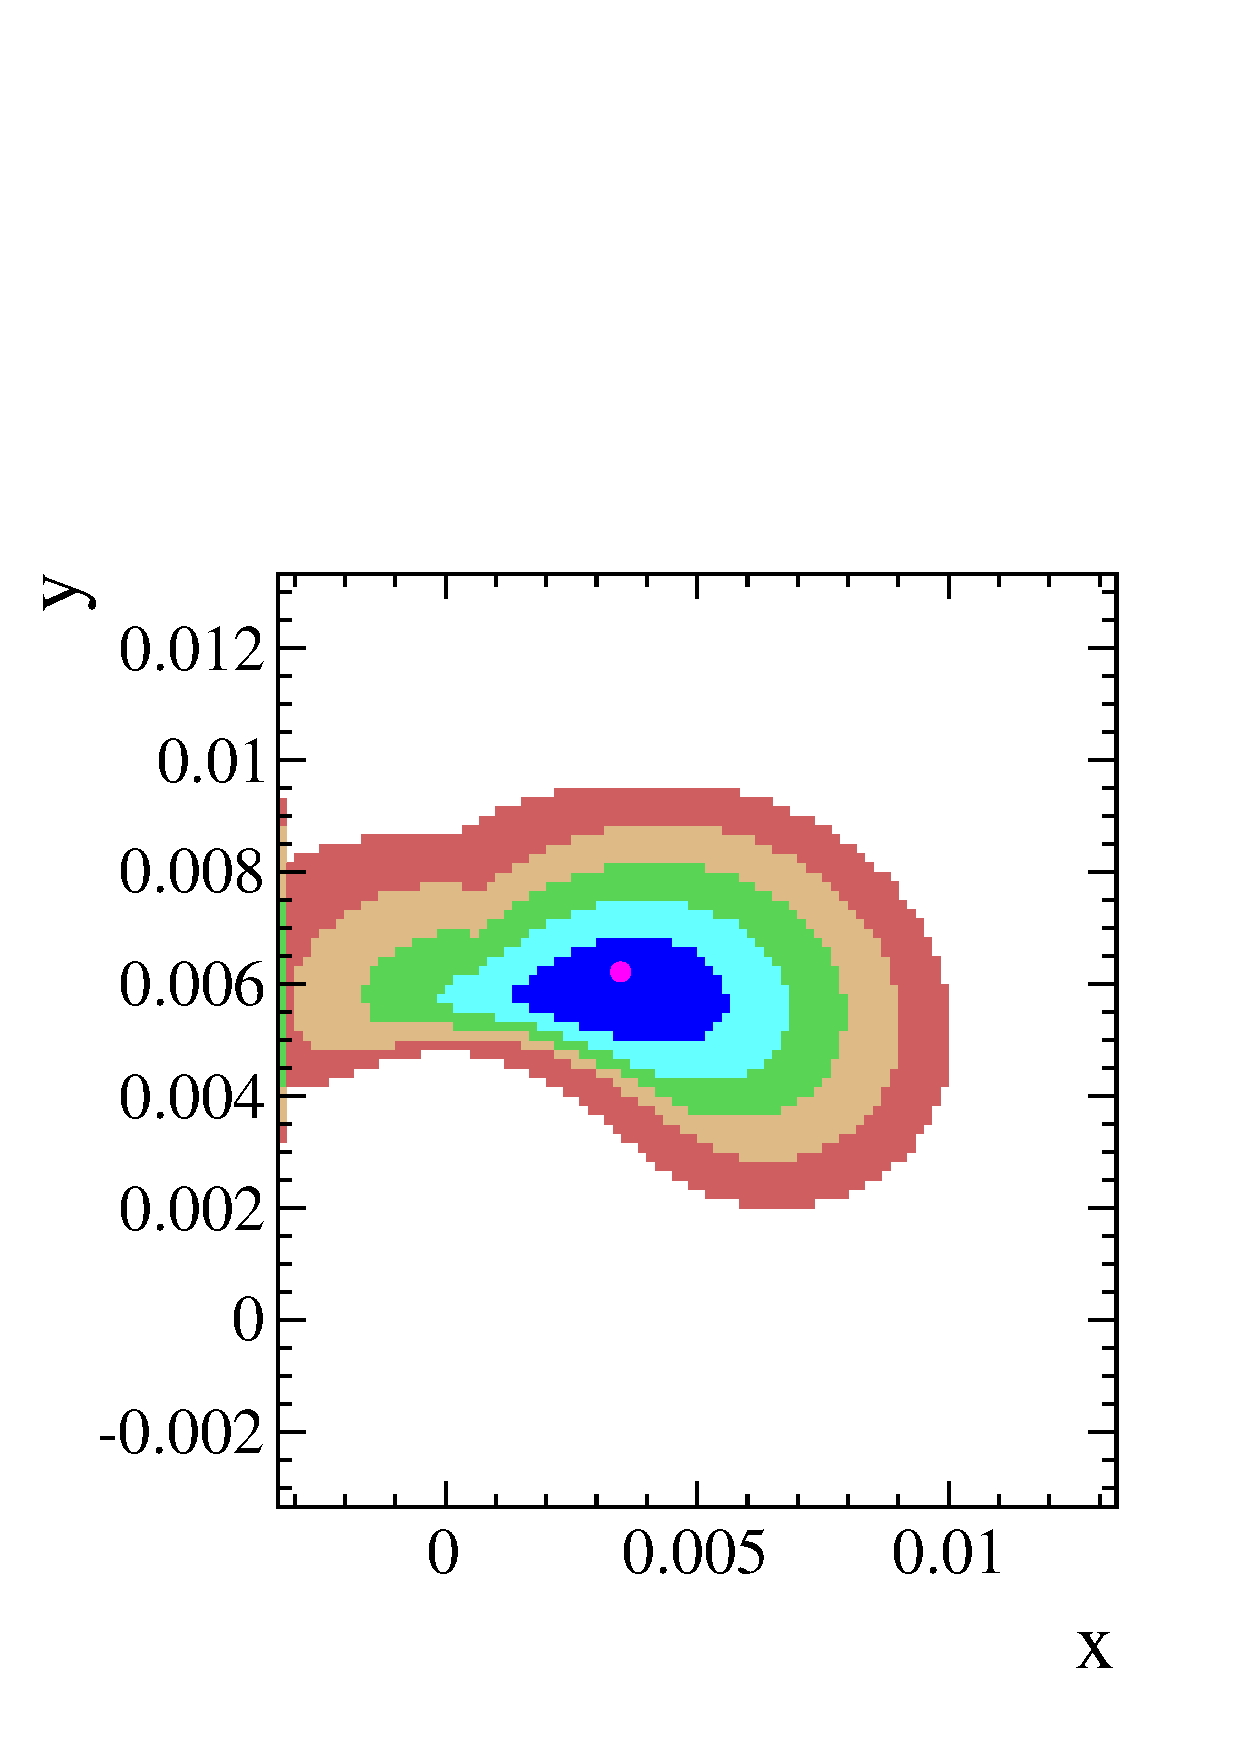
\includegraphics[width=\textwidth]{finalplot_allcpv_no_belle_babar_cdf_graph_lhcb_agamma.pdf}
%      \caption{Two dimensional error ellipses for x and y from fit excluding Belle, BaBar and CDF $K\pi$ results. Include latest $A_\Gamma$ result of LHCb.}
%      \label{fig:xy_all_cpv_with_agamma}
%    \end{subfigure}%
%    %\vspace*{-1.0cm}
%  \end{center}
%  \caption{Two dimensional error ellipses of fit for All CPV including differing sets of data for $x$ vs $y$. The biggest differences come from including the CDF result, which elongates the error ellipses. The differing colors represent the 1-5$\sigma$ contours.}
%  \label{fig:xy_all_variations}
%\end{figure}

%%%%%%%%%%%%%%%% Q/P %%%%%%%%%%%%%%%%%%%%%%%%%%%%%%%%%%%%
\begin{figure}[tb]
  \begin{center}
    \begin{subfigure}[b]{0.4\textwidth}
      \centering
      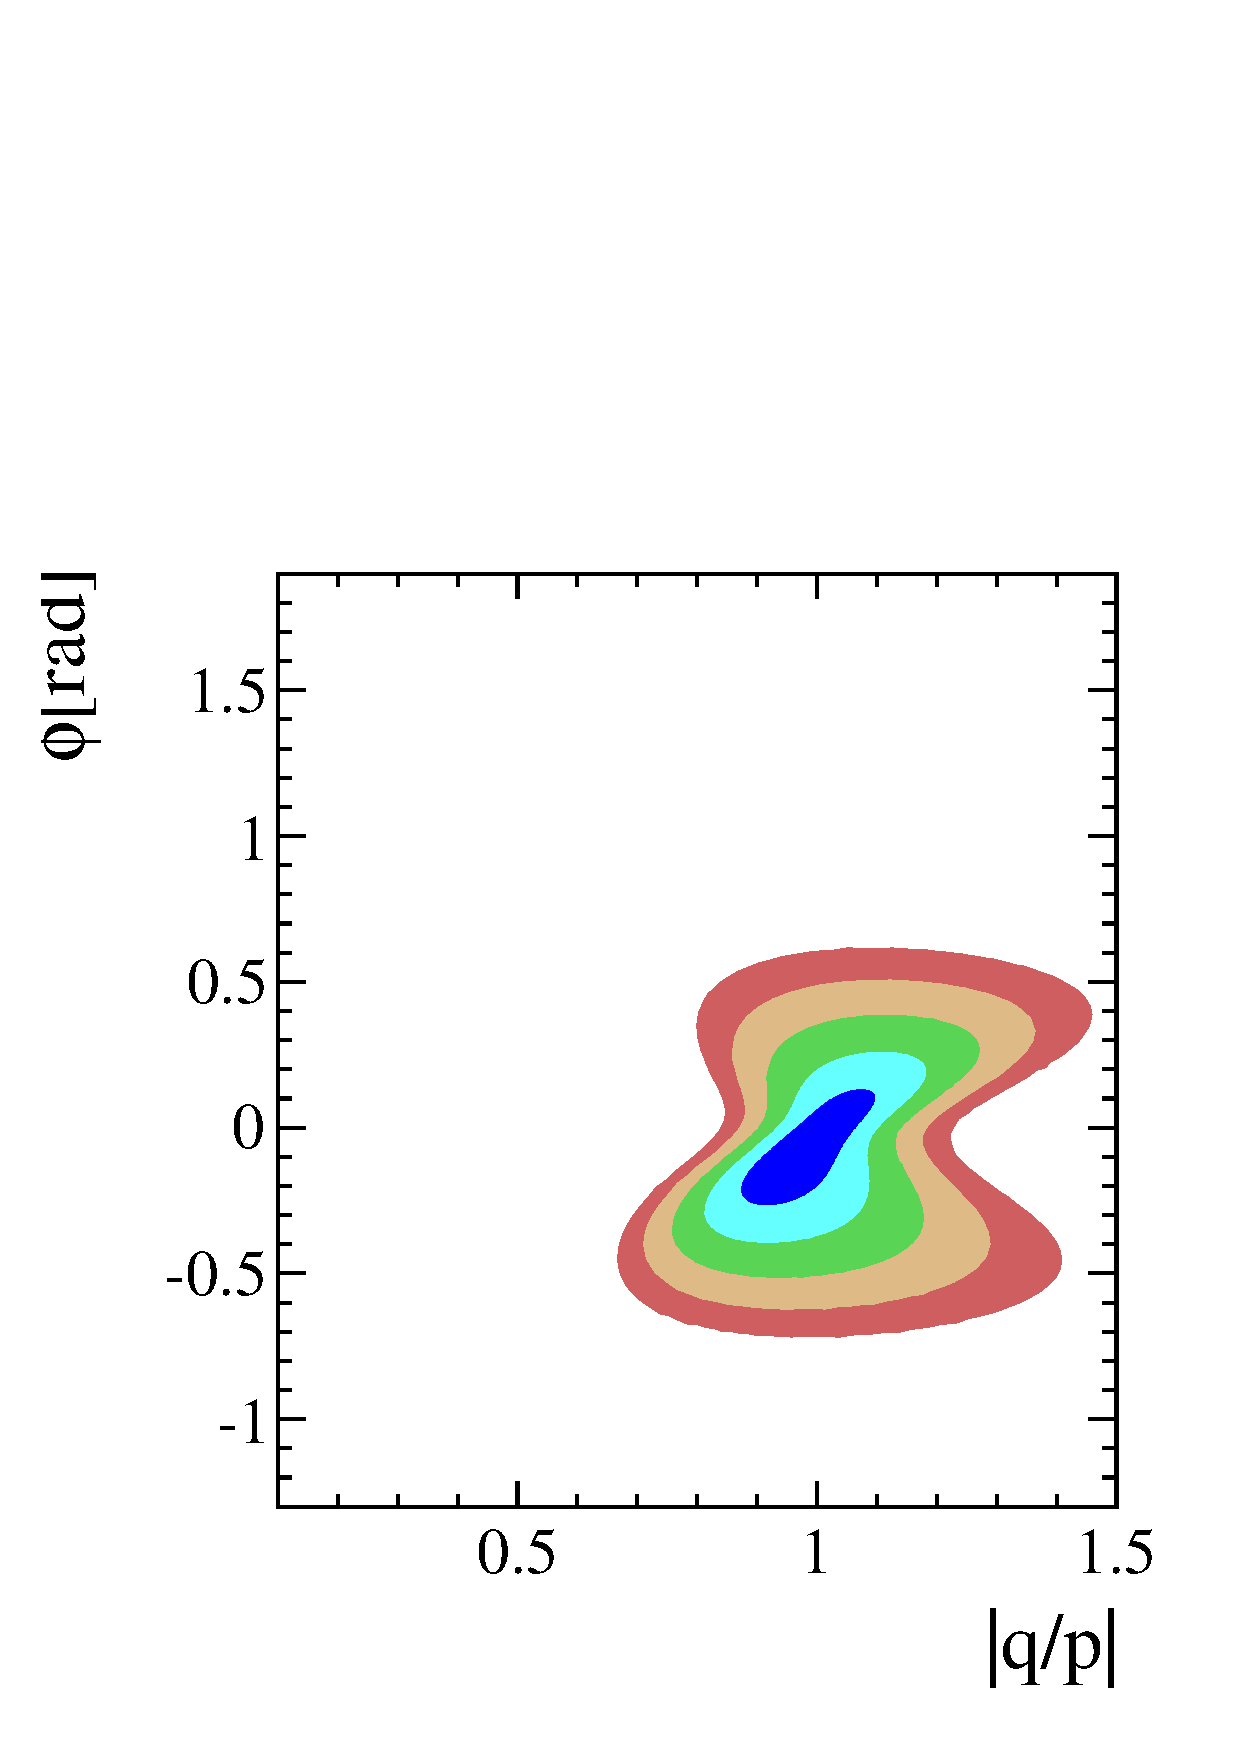
\includegraphics[width=\textwidth]{finalplot_allcpv_no_belle_babar_graph_qop_phi_hfag_agamma.pdf}
      \caption{Two dimensional error ellipses for x and y from fit excluding Belle and BaBar $K\pi$ results. Does not include latest $A_\Gamma$ result of LHCb.}
      \label{fig:xy_all_cpv_no_agamma}
    \end{subfigure}% 
    \hspace{2mm}
    \begin{subfigure}[b]{0.4\textwidth}
      \centering
      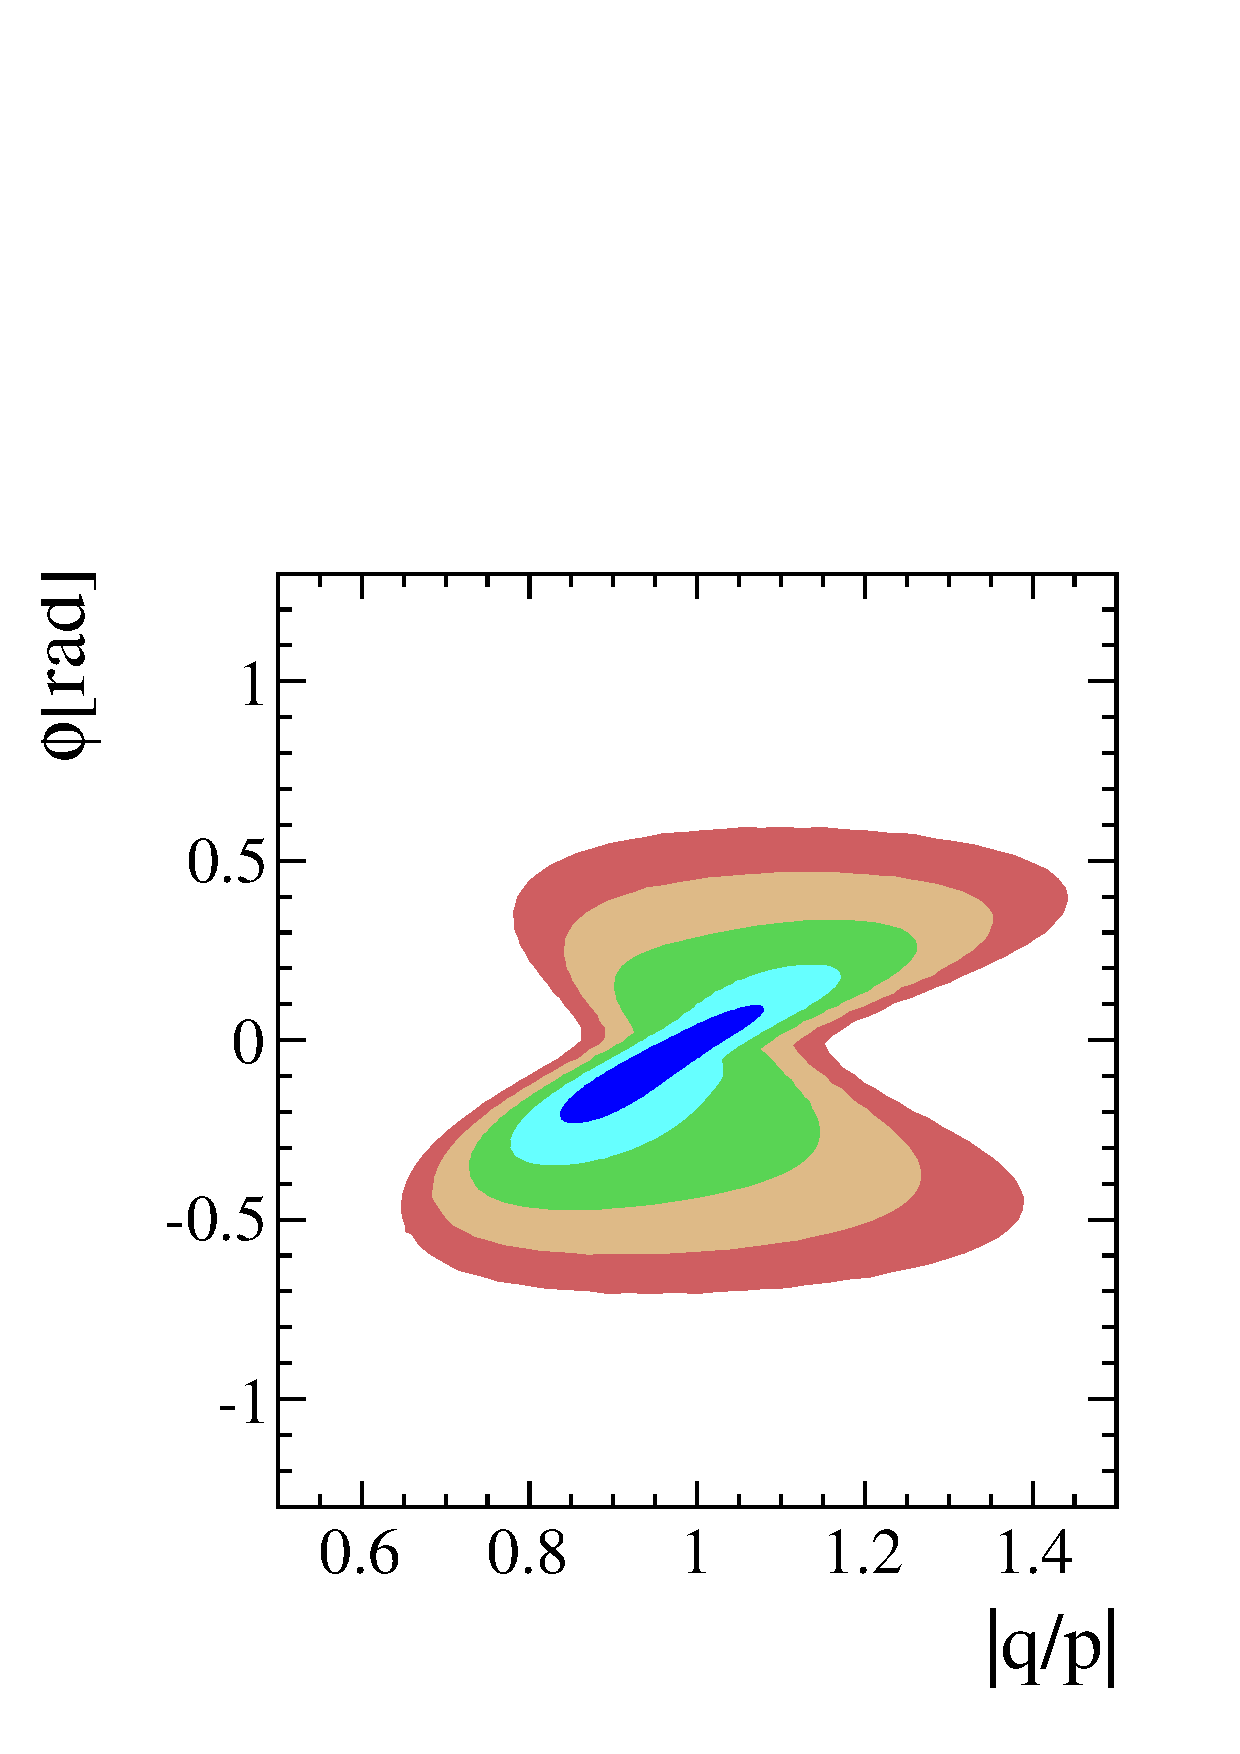
\includegraphics[width=\textwidth]{finalplot_allcpv_no_belle_babar_graph_qop_phi_lhcb_agamma.pdf}
      \caption{Two dimensional error ellipses for x and y from fit excluding Belle and BaBar $K\pi$ results. Include latest $A_\Gamma$ result of LHCb.}
      \label{fig:xy_all_cpv_with_agamma}
    \end{subfigure}%
%%%%%%%%%
        \\
    \begin{subfigure}[b]{0.4\textwidth}
      \centering
      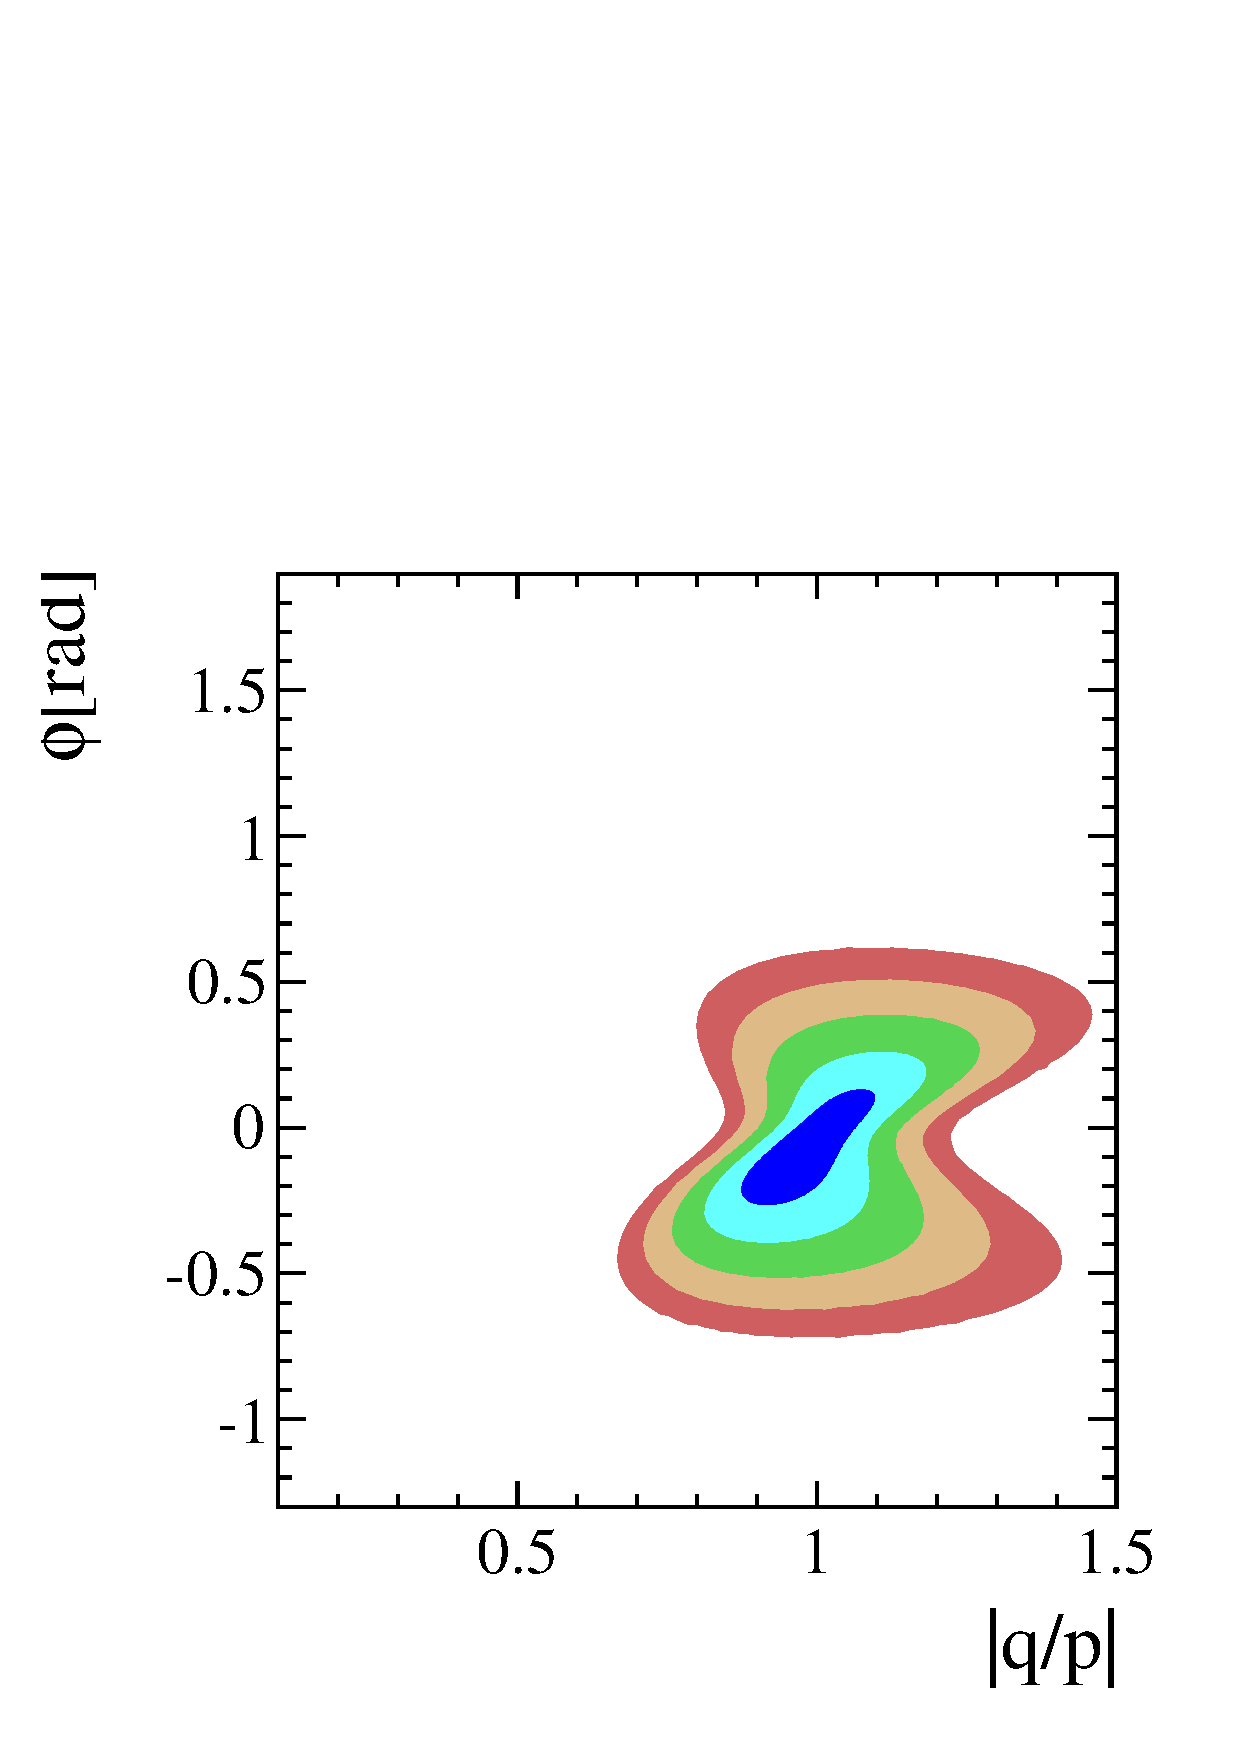
\includegraphics[width=\textwidth]{finalplot_allcpv_no_belle_babar_cdf_graph_qop_phi_hfag_agamma.pdf}
      \caption{Two dimensional error ellipses for x and y from fit excluding Belle, BaBar and CDF $K\pi$ results. Does not include latest $A_\Gamma$ result of LHCb.}
      \label{fig:xy_all_cpv_no_agamma}
    \end{subfigure}%
    \hspace{2mm}
    \begin{subfigure}[b]{0.4\textwidth}
      \centering
      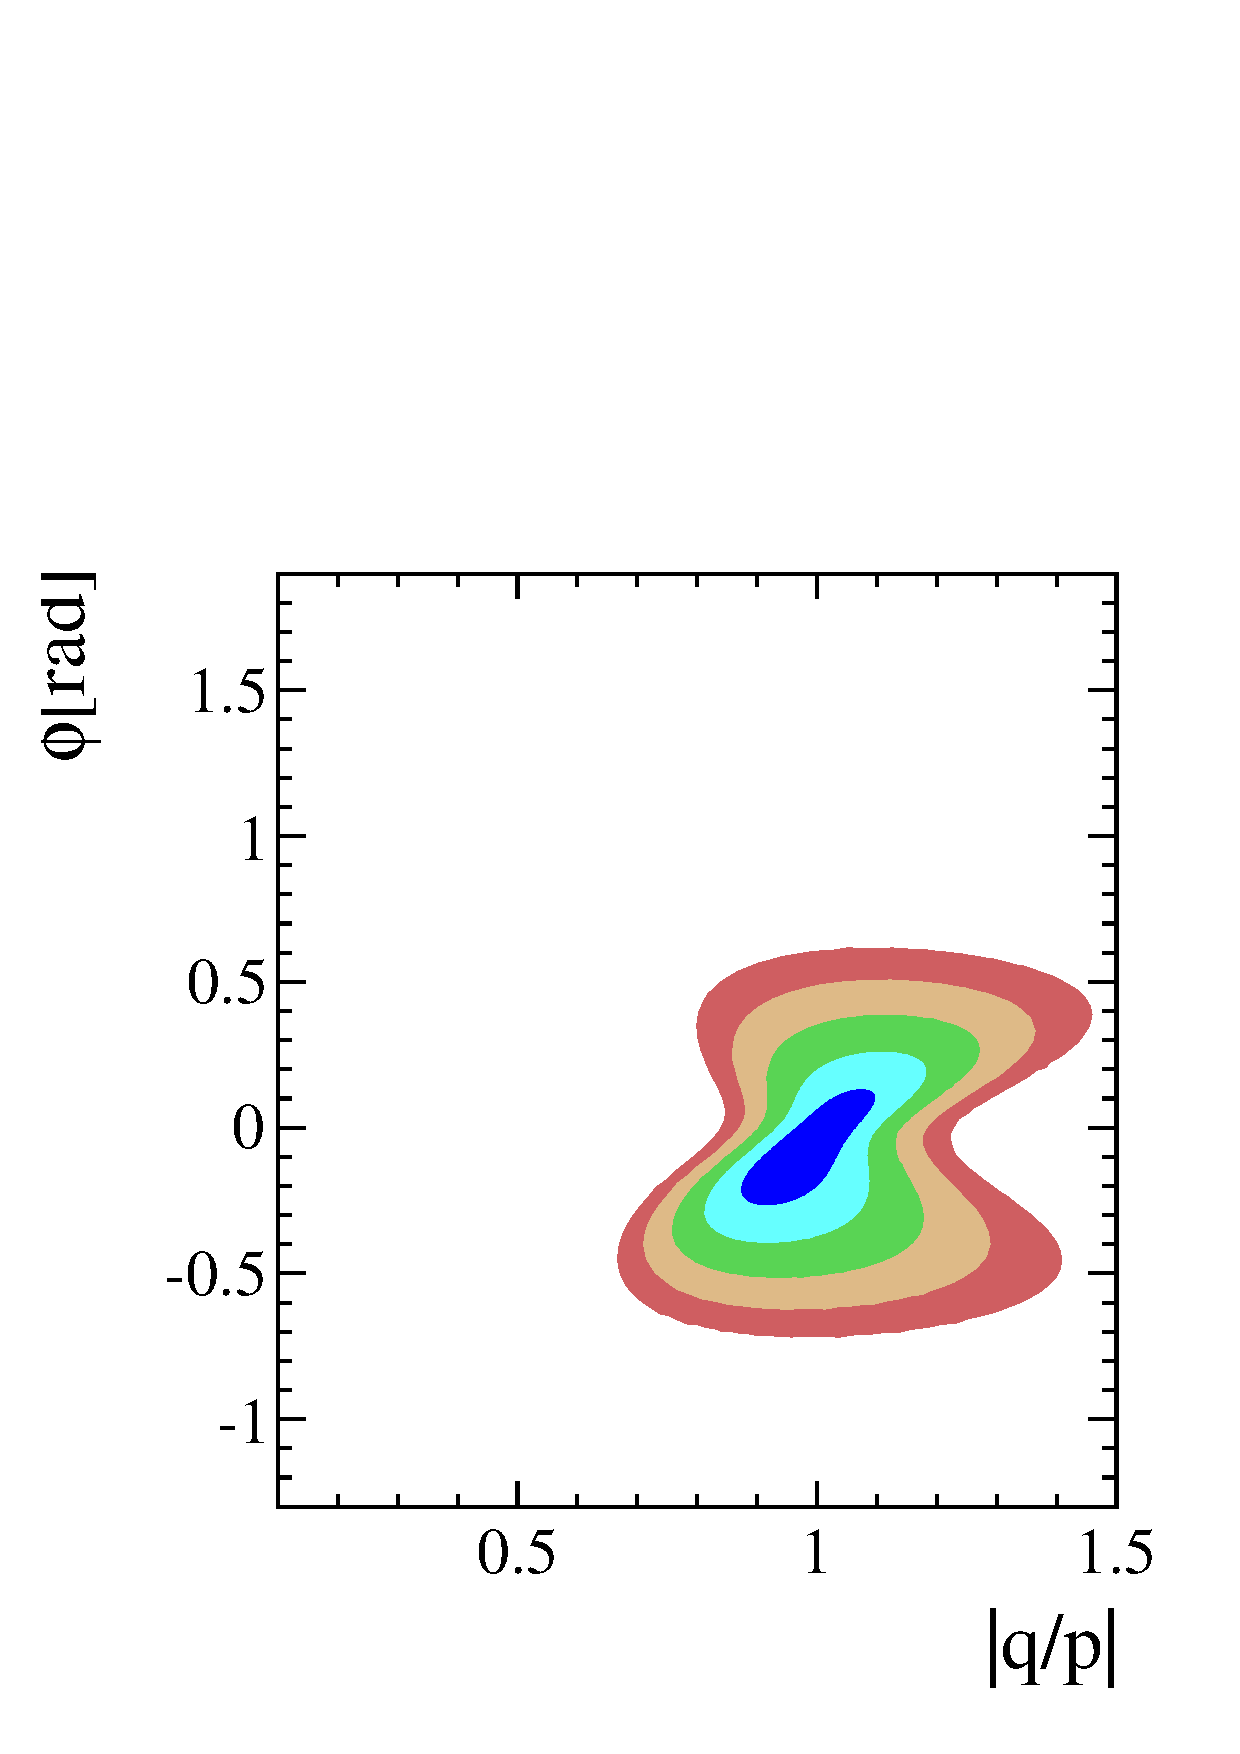
\includegraphics[width=\textwidth]{finalplot_allcpv_no_belle_babar_cdf_graph_qop_phi_lhcb_agamma.pdf}
      \caption{Two dimensional error ellipses for x and y from fit excluding Belle, BaBar and CDF $K\pi$ results. Include latest $A_\Gamma$ result of LHCb.}
      \label{fig:xy_all_cpv_with_agamma}
    \end{subfigure}%
    %\vspace*{-1.0cm}
  \end{center}
  \caption{Two dimensional error ellipses of fit for All CPV including differing sets of data for $\phi$ vs $q/p$. The biggest differences come from including the CDF result, which elongates the error ellipses. The differing colors represent the 1-5$\sigma$ contours.}
  \label{fig:xy_all_variations}
\end{figure}

\subsection{All CP Violation Allowed, Fit for $x_{12},y_{12},\phi_{12}$}
Table~\ref{table:allcpv_output_table_alex} lists the results for the All CPV allowed fit with the substitution of $x$ and $y$ for the underying parameters $x_{12},y_{12}$ and $\phi_{12}$. 
\begin{table}[htdp]
%\begin{tiny}

\begin{center}
\resizebox{16cm}{!} {
\begin{tabular}{|c||c||c||c||c|}
\hline
& All Measurements & No Belle, BaBar& No Belle, BaBar, $A_{\Gamma\text{ LHCb}}$ & No Belle, BaBar, CDF,$A_{\Gamma\text{ LHCb}}$ \\ \hline

$x_{12}(\times10^{-3})$&$ 3.789\pm1.627$  & $4.842\pm1.693$&$4.842\pm1.693$ & $4.853\pm1.694$\\ \hline

$y_{12}(\times10^{-3})$&$ 6.365\pm 0.953$  &$6.851\pm0.099$ & $6.851\pm 0.994$&$6.863\pm0.994$ \\ \hline

$\delta_{K\pi}(\times10^{-1})[\text{rad}]$&$1.855\pm 2.523$ & $3.237\pm1.949$& $3.237\pm1.949$&$3.191\pm1.950$ \\ \hline

$\phi_{12}(\times10^{-2})[\text{rad}]$&$-0.304\pm4.277$ &$-0.210\pm3.416$ & $-0.210\pm3.416$&$-0.249\pm3.380$ \\\hline

$R_D^-(\times10^{-3})$&$3.501\pm0.038$ & $3.556\pm0.043$& $3.556\pm0.043$& $3.556\pm0.043$\\ \hline

$R_D^+(\times10^{-3})$& $3.505\pm0.038$& $3.558\pm0.043$& $3.558\pm0.043$& $3.558\pm0.043$\\ \hline

$\chi^2/ndf$& 50.73/27&  19.5825/15& 19.5825/15& 8.62343/12\\ \hline

\end{tabular}
}
\end{center}
\caption{Output of the All CP Violation allowed global fit when fitting for the 
underlying parameters $x_{12}$ and $y_{12}$. Different Columns list 
differing subsets of data included in the fit.}
\label{table:allcpv_output_table_alex}
%\end{tiny}
\end{table}%



\section{Conclusion}
\label{sec:Conclusion}
By utilizing a global, HFAG-like fit, we constrain to be $|q/p| = xxxxx\pm yyyyy$ 
and $\phi = zzzzzzz\pm qqqqqqqqqqqqq$, 
in the case of all CPV allowed. Allowing only direct CPV, $|q/p| = xxxxx\pm yyyyy$
and $\phi = zzzzzzz\pm qqqqqqqqqqqqq$.
These measurements represent the most precise determination of the CP violating
parameters of the netural $D$ meson system


% Do not include this in analysis note and conference reports
%\section*{Acknowledgements}

The text below are the acknowledgements as approved by the collaboration
board. Extending the acknowledgements to include individuals from outside the
collaboration who have contributed to the analysis should be approved by the
EB and, if possible, be included in the draft of first circulation.
 
\noindent We express our gratitude to our colleagues in the CERN
accelerator departments for the excellent performance of the LHC. We
thank the technical and administrative staff at the LHCb
institutes. We acknowledge support from CERN and from the national
agencies: CAPES, CNPq, FAPERJ and FINEP (Brazil); NSFC (China);
CNRS/IN2P3 and Region Auvergne (France); BMBF, DFG, HGF and MPG
(Germany); SFI (Ireland); INFN (Italy); FOM and NWO (The Netherlands);
SCSR (Poland); MEN/IFA (Romania); MinES, Rosatom, RFBR and NRC
``Kurchatov Institute'' (Russia); MinECo, XuntaGal and GENCAT (Spain);
SNSF and SER (Switzerland); NAS Ukraine (Ukraine); STFC (United
Kingdom); NSF (USA). We also acknowledge the support received from the
ERC under FP7. The Tier1 computing centres are supported by IN2P3
(France), KIT and BMBF (Germany), INFN (Italy), NWO and SURF (The
Netherlands), PIC (Spain), GridPP (United Kingdom). We are thankful
for the computing resources put at our disposal by Yandex LLC
(Russia), as well as to the communities behind the multiple open
source software packages that we depend on.


%% $Id: appendix.tex 38562 2013-07-04 07:33:58Z tgershon $
% ===============================================================================
% Purpose: appendix to the standard template: standard symbol alises from Ulrik
% Author: Tomasz Skwarnicki
% Created on: 2009-09-24
% ===============================================================================

\clearpage

{\noindent\bf\Large Appendices}

\appendix

\section{Detailed Explanation}
\section{TupleToolExtraMu}
\label{sec:TupleToolExtraMu}
Looking explicitly for extra particles in the decay and asking whether or not these 
particles would satisfy the selection criteria for a given channel is done automatically 
by the DecayTreeTuple algorithm. However, it is beneficial to ask whether there are other 
particles which would satisfy the same selection criteria. The motivation behind writing 
the tool TupleToolExtraMu is to explicitly search for extra muons in an event which could 
be confused with, or be mis-associated as the true muon from the semileptonic decay 
$B\to \mu D^* X$. Storing additonal information about the ``extra" candidate then allows 
for a by-hand analysis of extra candidates.\\
TupleToolExtraMu configures as a tuple tool added to the DecayTreeTuple algorithm. By default, 
it outputs
\begin{itemize}
	\item The number of additional muons reconstructed from the TES location StdAllVeryLooseMuons, called extra muons
	\item The 4-momentum components of the extra muons
	\item The charge of the extra muon
	\item The Delta Log Likelihood distributions $\Delta \log( \mathcal{L}(\mu-\pi))$ and  $\Delta \log( \mathcal{L}(\mu-K))$ for the extra muon
	\item The Ghost Probability of the extra muon
	\item The extra muon Track Ghost Probability
	\item Extra muon Track $\chi^2/DoF$
	\item The invariant mass of the extra muon and the original muon being used
	\item The vertex $\chi^2$ and $DoF$ of the extra muon and original muon vertex
	\item The vertex $\chi^2$ and $DoF$ of the extra muon and the $D^*$ candidate
	\item The invariant mass of the extra muon and $D^*$ candidates
	\item The IP and IP$\chi^2$ of the extra muon
	\item Whether or not the extra muon originates from the same primary vertex as the $D^*$ candidate
\end{itemize}
This information allows one to, by hand, apply the stripping selections to the extra muons. 
The inclusion of the invariant mass distributions is meant to provide a tool in searching for 
additional sources of background. Figure~\ref{fig:nextra} shows the output of the number of 
extra muons summed over all events. The additional lines show the transformation of the number 
of additional candidate muons after applying cuts.

%%%%%%nextramu distributions%%%%%%%%%
\begin{figure}[tb]
  \begin{center}
	\includegraphics[width=0.49\linewidth]{rs_n_extra_muon_stripped} \put(-58,123){(a)}
	\includegraphics[width=0.49\linewidth]{rs_n_extra_muon_stripped_logy} \put(-58,123){(b)}
	\end{center}
  \caption{
    \small %captions should be a little bit smaller than main text                                                                                                                
    Distribution of $n(\mu_\text{Extra})$, the number of extra muons in a event, in (a) linear scale and (b) log scale. Different selection cuts are applied to extra muons to determine what fraction mis-association is to be expected.
    }
  \label{fig:nextra}
\end{figure}



% This should be taken out in the final paper
%\clearpage

\section{Supplementary material}
\label{sec:Supplementary-App}

This appendix includes supplementary material that will be 
  part of the draft during the review phase but will not appear in the
  final version of the paper. Instead it will be posted as supplementary
  material alongside the paper on CDS.

\begin{figure}[!htb]
  \begin{center}
    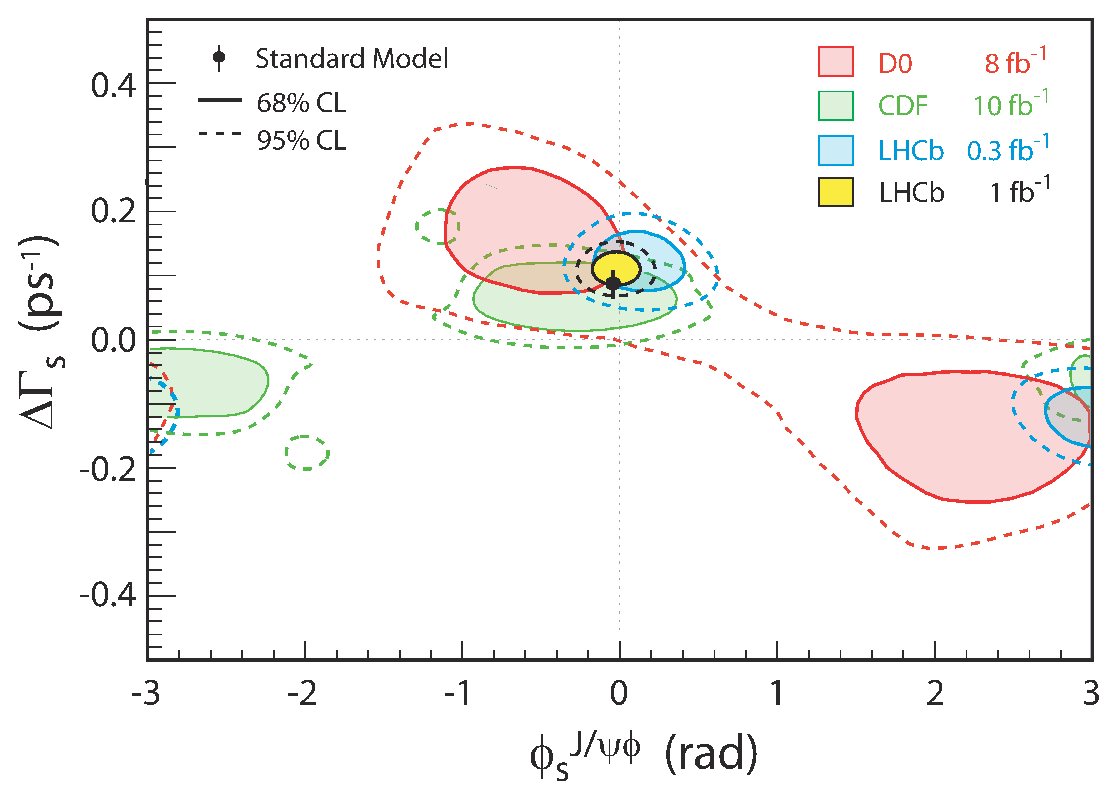
\includegraphics[scale=0.65,bb=50 300 580 700,clip=true]{Roger-plot}
    \vspace*{-1.0cm}
  \end{center}
  \caption{
    \small %captions should be a little bit smaller than main text
    Comparison of our result to those from other experiments.
    Note that the style of this figure differs slightly from that of Figure~\ref{fig:example}}
  \label{fig:roger}
\end{figure}

\clearpage


%\addcontentsline{toc}{section}{References}
%\setboolean{inbibliography}{true}
%\bibliographystyle{LHCb}
%\bibliography{main,LHCb-PAPER,LHCb-CONF,LHCb-DP}

\end{document}
